\documentclass[11pt]{article}
\usepackage[margin=1in]{geometry}
\usepackage{amsmath,amssymb,amsthm}
\usepackage{booktabs,tabularx,array}
\usepackage{graphicx}
\usepackage[hidelinks]{hyperref}
\usepackage{enumitem}
\usepackage{xcolor}
\usepackage[htt]{hyphenat}\sloppy
\setlist{itemsep=2pt,topsep=4pt}

\newtheorem{theorem}{Theorem}[section]
\newtheorem{proposition}[theorem]{Proposition}
\newtheorem{corollary}[theorem]{Corollary}
\newtheorem{lemma}[theorem]{Lemma}
\theoremstyle{definition}
\newtheorem{definition}[theorem]{Definition}
\newtheorem{construction}[theorem]{Construction}
\newtheorem{observation}[theorem]{Observation}
\newtheorem{counterexample}[theorem]{Counterexample}
\newtheorem{problem}[theorem]{Problem}
\newtheorem{conjecture}[theorem]{Conjecture}
\theoremstyle{remark}
\newtheorem{remark}[theorem]{Remark}

\newcommand{\Z}{\mathbb{Z}}
\newcommand{\Q}{\mathbb{Q}}
\newcommand{\R}{\mathbb{R}}
\newcommand{\F}{\mathbb{F}}
\newcommand{\CF}{\mathrm{CF}}
\newcommand{\NCF}{\mathrm{NCF}}
\newcommand{\lmin}{\ell_{\min}}
\newcommand{\one}{\mathbf{1}}
\newcommand{\KL}{D_{\mathrm{KL}}}
\newcommand{\Aff}{\mathrm{Aff}}
\newcommand{\src}[1]{\textsf{\small[#1]}}
\newcommand{\st}[1]{\textsf{\small\color{gray}#1}}

\title{Three layers of realisation:\\ hierarchy recovery, holonomy, information and contextuality}
\author{Vinay Awasthi\\ \small Department of Applied Mathematics and Statistics, Johns Hopkins University}
\date{}

\begin{document}
\maketitle

\begin{abstract}
This paper consolidates three bodies of work into one account. Each result carries its source and its status: proved, computed, measured, open, or closed by theorem.
\begin{enumerate}
  \item \emph{Hierarchy recovery} \src{H}. A gradient-free estimator (spectral initialisation, soft hand-off, inside--outside EM and split--merge) recovers a depth-4 probabilistic grammar to $0.001$ nats per sequence of the true model in 131\,s. Twelve transformer configurations never represent the level-3 latent symbol.
  \item \emph{Cohomological strand} \src{O}. Holonomy of known operations gives a genuine obstruction $[g]\in H^1(\Gamma,A)$. Marginal obstructions within one data source vanish (T0). The information site and the contextuality site are separated by a theorem.
  \item \emph{Results of the present work} \src{S}:
  \begin{itemize}
    \item an exact identifiability criterion for holonomy estimated from data, with a calibrated test and its sample cost;
    \item a direct construction from operations to outcomes, $[g]\ne0\iff\gamma\ne0$, which is invisible to the probability layer;
    \item for lossy operations: a closed form $\CF=\max(0,1-|L|\varepsilon/2)$ on a cycle, and a holonomy-girth lower bound on general graphs;
    \item the loop spectrum as a monoid-valued holonomy invariant;
    \item a decorated Bregman--\v{C}ech nerve that carries orientation and phase, with a codimension criterion for when it can;
    \item restriction and extension maps between the information and contextuality views;
    \item a gated contextuality test for streams with \emph{not-applicable} entries, with a pinned maximum-likelihood null.
  \end{itemize}
\end{enumerate}
The organising statement is that the three layers (operations, probability and outcomes) respond to the same data through different invariants, and that no invariant of one layer determines another.
\par\smallskip\noindent\textbf{Code:} \url{https://github.com/vkawasth/Trainingless-Transformer-NoGradientDescent/tree/main/AMB-Vigneaux/}
\end{abstract}

\noindent\textbf{Provenance tags.}
\begin{itemize}
  \item \src{H}: \emph{Recovering latent hierarchy without gradient descent} (hierarchy paper and handoff).
  \item \src{O}: \emph{Holonomy obstructions for composed local operations} (holonomy paper).
  \item \src{S}: this work, implemented in the \texttt{amb\_vigneaux} package. It has 107 tests, and every numerical claim tagged \src{S} is produced by that code.
\end{itemize}
\noindent\textbf{Status tags:} \st{proved}, \st{computed} (exact computation or verified identity), \st{measured} (empirical, no proof), \st{open}, \st{closed} (settled by theorem, not to be reopened).

\tableofcontents
\newpage

%=====================================================================
\section{The standing constraint}

\begin{theorem}[T0: single-source global section]\label{thm:T0}
\src{O, Thm 7} \st{proved}
Let $\{P_C\}_{C\in\mathcal M}$ be context marginals estimated from one sample $\mathcal D$. The empirical joint $P_{\mathcal D}$ restricts to each $P_C$, so the family extends. Consequently the \v{C}ech obstruction $\gamma(s)$ vanishes for every section and the contextual fraction is $0$, on any cover, acyclic or not.
\end{theorem}
\begin{proof}
$P_{\mathcal D}$ is a global section by construction.
\end{proof}

\begin{corollary}\label{cor:T0}
\src{H/O} \st{proved}
A single fitted model can never exhibit an obstruction to its own consistency. If an estimator and a detector share a data source, the detector measures model misfit, not structure.
\end{corollary}

\begin{remark}[T0 as a functor]
\src{S} \st{proved}
Restriction $R$ from global laws to context families (Section~\ref{sec:functors}) has image exactly the non-contextual models. So T0 is the statement that anything in the image of $R$ has $\CF=0$ and $\gamma=0$. The engine's first version violated T0 by resampling a single-source world context by context: it produced a spurious $\CF$ up to $0.10$, and the fitted model's $\CF$ equalled its signalling defect exactly. After adding a single-source sampling mode, $\CF(\hat P_N)\le2\times10^{-16}$.
\end{remark}

%=====================================================================
\section{The three layers}

\begin{table}[h]\centering
\begin{tabularx}{\linewidth}{@{}l>{\raggedright}X>{\raggedright\arraybackslash}X@{}}
\toprule
Layer & Invariant & Condition for non-triviality\\
\midrule
1 Operations & $H^1(\Gamma,A)\cong A^{\beta_1}$, holonomy; the loop spectrum for lossy operations & The operations are known or identifiable (Prop.~\ref{prop:ident}); $\beta_1>0$\\
2 Probability & $H^1(\mathcal S;\mathcal F_\alpha)$, one-dimensional, generated by entropy (Tsallis for the $\alpha$-action) & The conditioning action is present; $I=\delta_tH$ measures its failure to be trivial\\
3 Outcomes & $\gamma\in\check H^1(\mathcal U,\mathcal F_{\tilde C})$; $\CF$ & The cover has no global context; data come from more than one source (T0)\\
\bottomrule
\end{tabularx}
\caption{The stratification \src{O, \S6}, extended \src{S}.}
\end{table}

\begin{remark}[Stratification, not bridge]
\src{O, Rem.~18} \st{proved}
Each invariant is non-trivial on its own layer and zero on the others, and the reasons are the hypotheses themselves. Layer~2's site has a global joint, which gives the observable monoid an absorbing element; Theorem~\ref{thm:vanish} then kills every trivially-acting coefficient system, which is where Layer~3's coefficients would have to live. Layer~3's site is built so that no global context exists. That is what permits $\gamma\neq0$, and it simultaneously denies Layer~2 the joint it requires.

\src{S} adds that the layers are connected \emph{around} Layer~2, not through it. There is an exact construction from Layer~1 to Layer~3 (Theorem~\ref{thm:eg}), and Layer~2 is provably blind to it (Proposition~\ref{prop:blind-eg}).
\end{remark}

%=====================================================================
\part{Hierarchy recovery \src{H}}
\section{Setup and exact floors}

All experiments use the Random Hierarchy Model of Cagnetta et al.~\cite{cagnetta}. It is a probabilistic context-free grammar on a fixed complete binary tree of depth $L$, with $V$ symbols per internal level, $m$ productions per symbol, and a leaf alphabet of size $A$. Because the tree shape is fixed and positional, the latent structure is a Markov chain from leaves to level 1 and on up to the root.
\begin{itemize}
  \item \emph{Corpus A}: $L=4$, $V=64$, $A=48$, $m=12$, $2\times10^5$ sequences of length 16.
  \item \emph{Corpus B}: $L=4$, $V=8$, $A=12$, $m=3$, $2\times10^5$ sequences.
\end{itemize}
The exact conditional entropy $H(x_t\mid x_{<t})$ is computed by inside--outside (Theorem~\ref{thm:io}). For Corpus A: $H_{\text{local}}=1.6034$, $H_{\text{higher}}=3.5527$, $H(x_0)=3.8161$ nats. The latent-symbol entropies given the prefix, for levels 1--4, are $2.7835,2.2923,2.2900,2.7910$ against chance $\ln V=4.1589$. About $1.87$ nats of level-3 information are recoverable from the prefix.

\section{Transformers do not recover levels 3--4}
\begin{table}[h]\centering\small
\begin{tabular}{lccc}
\toprule
configuration & local & higher & level-3 probe\\
\midrule
2 layers, $d=64$ (baseline) & 2.173 & 3.831 & 0.028\\
4 layers & 2.078 & 3.797 & ---\\
8 layers, frozen embedding & 2.037 & 3.755 & ---\\
8 layers, frozen emb., fresh sampling & 2.022 & 3.772 & 0.027\\
$d=128$, 4 layers & 2.039 & 3.770 & ---\\
frozen random embedding (2 layers) & 2.186 & 3.824 & ---\\
constructed order coordinate & 2.162 & 3.815 & ---\\
auxiliary supervision, levels 3--4 & 2.088 & 3.777 & 0.056\\
latent marginalising head (stopped at 34k) & 3.227 & 3.835 & ---\\
dilated causal CNN & 2.104 & 3.827 & 0.032\\
curriculum over tree depth & 2.085 & 3.803 & 0.034\\
curriculum control (no easy cases) & 2.043 & 3.789 & 0.033\\
\midrule
exact floor & \textbf{1.603} & \textbf{3.553} & ---\\
\bottomrule
\end{tabular}
\caption{Corpus A, 48{,}000 steps each. Shuffled-label controls read $0.021$--$0.034$; chance is $1/V=0.0156$. \src{H}}
\end{table}

\noindent\textbf{Statement} \src{H} \st{measured}. Across twelve configurations the level-3 probe never leaves the shuffled-label floor, although 1.87 nats of level-3 information are present in the prefix. A linear probe on the embedding was \emph{withdrawn}: a random matrix supports the same probe accuracy.

\noindent\textbf{Hypothesis (not established).} Recovering the level-$\ell$ symbol requires marginalising over the parses consistent with the prefix. A feedforward stack has only an upward pass, while inside--outside couples an upward and a downward pass.

\section{The estimator and its verification}
\begin{construction}[Estimator]\src{H}
\begin{enumerate}
  \item \emph{Spectral initialisation}: build the pair--context co-occurrence matrix, take its leading singular directions, and $k$-means the pairs into $V$ groups.
  \item \emph{Soft hand-off}: pass the posterior to the next level, $q_\ell\propto\sum_{x,y}P_\ell[\cdot,x,y]\,q^{\text{lo}}_{\ell-1}(x)\,q^{\text{hi}}_{\ell-1}(y)$.
  \item \emph{EM}: inside--outside E-step and normalised-counts M-step, keeping the sweep with the best held-out likelihood.
\end{enumerate}
\end{construction}

\begin{table}[h]\centering\small
\begin{tabular}{llc}
\toprule
check & statement & max error\\
\midrule
V0 & EM never decreases the training log-likelihood & $+1.8\times10^{-2}$ (min step)\\
V1a & a free subtree has inside value exactly 1 & $1.8\times10^{-15}$\\
V1b & restriction = marginalisation & $8.9\times10^{-16}$\\
V1c & gluing = independence join, $P(x_{0:16})=\sum_{u,v}\mu(u,v)\beta_L(u)\beta_R(v)$ & $1.0\times10^{-14}$\\
V2 & the soft hand-off is a sufficient statistic & $6.7\times10^{-16}$\\
V4a & merge cost $=N\,I(\text{children};B\mid q(B))$ & $1.2\times10^{-14}$\\
\bottomrule
\end{tabular}
\caption{Identities of the tree model class \src{H} \st{computed}. They verify the implementation and that the fitted object is a sheaf section. They do not test whether the data are tree-generated. The hard (argmax) decode flips on 34--46\% of sequences under a chain of conditionings; the soft decode does not change.}
\end{table}

\begin{table}[h]\centering\small
\begin{tabular}{lccc}
\toprule
variant (Corpus A, $2\times10^4$ sequences) & local & higher & held-out $\log p$/seq\\
\midrule
joint EM from random init & 2.566 & 3.831 & $-51.18$\\
bottom-up, frequency-rank clusters & 2.598 & 3.833 & $-51.45$\\
spectral + soft hand-off + EM (10 sweeps) & 2.227 & 3.802 & $-48.23$\\
spectral + soft hand-off + EM (50 sweeps) & 2.162 & 3.807 & $-47.75$\\
stagewise + vertical re-clustering & 2.240 & 3.802 & $-48.34$\\
\midrule
transformer, 48k steps & 2.022 & 3.772 & ---\\
true grammar & 1.599 & 3.553 & $-41.21$\\
\bottomrule
\end{tabular}
\caption{Estimator variants on Corpus A \src{H}.}
\end{table}

\section{Instruments for detecting hierarchy}
\begin{itemize}
  \item \textbf{V6, leaf pairs} \src{H} \st{measured}. The test is a parametric bootstrap of empirical mutual information against datasets sampled from the fitted model.
  \begin{itemize}
    \item \emph{Planted positive}: copying leaf 7 into leaf 8 with probability $0.3$ gives $z=+220$, against $+6.5$ elsewhere; even the true grammar is refuted there ($z=+390$).
    \item \emph{Limitation}: on Corpus A, pairwise leaf MI across level-2 and root boundaries is about $10^{-4}$ even under the true grammar, while the plug-in bias floor is about $0.055$. So V6 has no power above level 1.
  \end{itemize}
  \item \textbf{V7, blocks} \src{H} \st{measured}. Each block is decoded by its own inside vector, and adjacent blocks are compared under the disjointness invariant.
  \begin{itemize}
    \item Decoded with the true grammar, blocks sharing a parent carry about 1 nat, and others $0.002$--$0.014$.
    \item The fitted model captures 79\%, 1.4\% and 3.9\% of this at levels 1--3.
  \end{itemize}
  \item \textbf{$\beta_1$ of the block complex} \src{H} \st{measured}. A tree predicts $\beta_1=0$ at every threshold.
  \begin{itemize}
    \item Corpus B, unplanted: $0$ at all 25 thresholds.
    \item Two planted block couplings: $\beta_1=1$ at 5 thresholds, with the null at $0$. A single coupling never produces a cycle.
    \item $\beta_1$ is computed on a Rips complex, so it is a calibrated statistic and not an approximation to \v{C}ech persistence (Theorem~\ref{thm:ew}).
  \end{itemize}
\end{itemize}

\section{The regime determines learnability}
\begin{table}[h]\centering\small
\begin{tabular}{lcccc}
\toprule
 & level 1 & level 2 & level 3 & level 4\\
\midrule
Corpus A: observations per parameter & 1.4 & 0.31 & 0.15 & 0.08\\
Corpus B: observations per parameter & 1389 & 1563 & 781 & 391\\
\bottomrule
\end{tabular}
\caption{Identifiability regime \src{H}. Levels fail at 0.15 observations per parameter and succeed at 781.}
\end{table}
On Corpus B at 200 sweeps, the level-3 block dependence captured rises from $0.0854$ to $0.1827$, and its discrepancy falls from $z=+20.2$ to $+5.4$. The earlier failure was therefore an unestimable regime, then undertraining. Merges at levels 1--3 cost real conditional MI; the root alphabet is redundant, with $8\to2$ improving held-out likelihood by $0.004$.

\section{Closing the gap: basin selection and split--merge}
\begin{table}[h]\centering\small
\begin{tabular}{lcc}
\toprule
start & held-out $\log p$/seq & local / higher\\
\midrule
exact truth ($\varepsilon=0$) & $-15.324$ & 0.3322 / 1.5833\\
truth + 50\% / 80\% / 90\% uniform & $-15.325$ / $-15.325$ / $-15.330$ & ---\\
truth + 95\% / 99\% uniform & $-15.775$ / $-18.113$ & ---\\
uniform & $-20.706$ & 0.5091 / 2.0791\\
spectral init (ours) & $-17.511$ & 0.3952 / 1.7937\\
\bottomrule
\end{tabular}
\caption{Diagnosis: EM started at the truth \src{H} \st{measured}. The truth is a fixed point with a very wide basin.}
\end{table}

\noindent A hard partition of observed child pairs cannot represent a grammar in which pairs are shared across parents (4 of 16 at level 1).
\begin{itemize}
  \item Sharpening the clustering hurts: sibling context gives $-18.06$.
  \item Blurring it helps: blending with uniform at weight 0.9 gives $-15.87$.
\end{itemize}

\begin{construction}[Split--merge]\src{H}
For each level:
\begin{enumerate}
  \item duplicate the symbols with a perturbation;
  \item run EM;
  \item greedily merge back by Bregman information over \emph{all} $2V$ symbols, so merges can recombine across the split;
  \item accept only if held-out likelihood improves.
\end{enumerate}
\end{construction}
\begin{table}[h]\centering\small
\begin{tabular}{lcc}
\toprule
stage & held-out $\log p$/seq & merge cost (nats/seq), levels 1--4\\
\midrule
warmup, 40 EM sweeps & $-17.187$ & ---\\
round 1 & $-15.491$ & 0.160, 0.113, 0.008, 0.003\\
round 2 & $-15.325$ & 0.042, 0.011, 0.007, 0.005\\
round 3 & $-15.3253$ & 0.052, 0.020, 0.007, 0.004\\
true grammar & $\mathbf{-15.3243}$ & ---\\
\bottomrule
\end{tabular}
\caption{Split--merge on Corpus B \src{H} \st{measured}: 131\,s, local/higher $0.3322/1.5835$ against a true $0.3322/1.5833$.}
\end{table}

The recovered model passes all four instruments:
\begin{itemize}
  \item V3 matches the true column at every boundary.
  \item V6 flags 0 of 18 pairs, with largest $|z|=1.7$.
  \item V7 at level 3 reads $0.5863/0.5882$ against a true $0.6140$.
  \item $\beta_1$ against the fitted null is 0 of 25, where the local-optimum fit gave 6 of 25.
\end{itemize}

\section{Why clustering is necessary at scale}
A dense inside pass costs about $2NV^3$. At $N=10^6$ and $V=1024$ a sweep costs about $4.3\times10^{15}$. Compression to $K=16$ gives about $8\times10^{11}$ over 50 sweeps, a speedup of $(V/K)^3=262{,}144$. For $m$-ary grammars the order rises to $m+1$, so compression buys $\log_KV$ orders of headroom.

Compression is not free. Merge costs are level-dependent and must be measured, not assumed; V4a supplies the measurement. At $L=16$ the root is observed only about 15 times per $10^6$ tokens, so compression removes the compute barrier but not the identifiability barrier.

\section{O6 baseline: where split--merge breaks}\label{sec:o6}
We built O6 as a benchmark (\texttt{benchmarks/o6}). It consists of:
\begin{itemize}
  \item a seeded RHM generator that exports the true latent symbol of every test node;
  \item a scorer that reports the held-out likelihood gap and, at each level, the NMI of the model's MAP symbol against the truth, beside the true grammar's own (Bayes-ceiling) recovery;
  \item tiers O6-S ($V{=}64$, $L{=}8$), O6-M ($256$, $12$) and O6-L ($1024$, $16$).
\end{itemize}
We ran our gradient-free baseline up a ladder on 2 CPUs with 7\,GB of memory. The baseline is dense inside--outside EM with split--merge.
\begin{center}\small
\begin{tabular}{llccc}
\toprule
rung & protocol & test gap (nats/seq) & top-level recovery (model / ceiling) & s/sweep\\
\midrule
$V{=}16,L{=}4$ & full & $0.020$ & $0.55/0.88$ & $1.4$\\
$V{=}32,L{=}4$ & short & $0.150$ ($0.237$ with $4\times$ data) & $0.69/0.98$ & $8.3$\\
$V{=}64,L{=}4$ & short & $1.488$ & $0.72/0.99$ & $40$\\
$V{=}128,L{=}4$ & --- & out of memory once split & --- & $180$\\
$V{=}8,L{=}6$ & full & $0.005$ & $0.39/0.74$ & $2.0$\\
$V{=}8,L{=}8$ & full & $2.11$ & $0.41/0.77$ & $0.8$\\
$V{=}8,L{=}10$ & short & $60.7$ & $0.03/0.60$ & $0.8$\\
\bottomrule
\end{tabular}
\end{center}
Findings:
\begin{itemize}
  \item \emph{Likelihood does not certify structure.} Near-truth likelihood, with gaps of $0.02$ and $0.005$, coexists with top-level recovery far below the ceiling, because the top of the hierarchy carries little likelihood. The benchmark therefore scores structure first.
  \item \emph{Where it breaks.} Optimisation breaks at $V\approx64$: four times more data did not help at $V{=}32$. Memory breaks at $V{=}128$. Top-level structure fails from $L\approx6$--$8$, and the full protocol repairs likelihood but not the top two levels.
  \item \emph{Scaling.} Time per sweep grows as $V^{2.17}$. O6-S is beyond this hardware, at an estimated week or more.
  \item \emph{O6-L needs a sparse or structured parameterisation, whatever the optimiser.} Dense tables have $1.8\cdot10^{10}$ parameters and about $10^{-4}$ observations per top-level parameter at $N=10^5$. The true grammar has $3072$ rules per level.
\end{itemize}
The baseline, the generator and the scorer are released so that other methods can be run on the same footing.

\section{Theorems and constructions used \src{H}}
\begin{theorem}[Inside--outside; Baker, Lari--Young]\label{thm:io}\st{used}
For a PCFG on a fixed tree, the inside values $\beta$ and outside values $\alpha$ give exact marginals: the posterior at a node is $\propto\alpha\beta$.
\end{theorem}
\begin{theorem}[EM ascent; Dempster--Laird--Rubin]\label{thm:em}\st{used}
Each EM iteration does not decrease the observed-data log-likelihood.
\end{theorem}
\begin{theorem}[Convergence; Wu]\st{used}
Under regularity conditions, EM converges to a stationary point, and the limit depends on the initialisation.
\end{theorem}
\begin{theorem}[Extension; Vorob'ev]\label{thm:vorobev}\st{used}
Every consistent family of marginals on a hypergraph extends to a global distribution if and only if the hypergraph is acyclic. A fixed tree is acyclic.
\end{theorem}
\begin{theorem}[Independent pullback; Simpson Thm 6.4, Prop.~8.5]\st{used}
A presheaf on standard Borel probability spaces is an atomic sheaf iff it maps independent squares to pullbacks. The independent pullback is the conditional product.
\end{theorem}
\begin{definition}[Supports; Simpson Def.~7.1] A support of a random variable is its terminal factorisation through a sample space.\end{definition}
\begin{theorem}[Conditional products; Fritz \S12]\st{used}
In a Markov category with conditionals, conditional products exist and satisfy the Dawid--Studen\'y axioms. $\mathsf{FinStoch}$ is such a category.
\end{theorem}
\begin{theorem}[Sufficient statistics; Fritz Def.~14.3, Thm~14.5]\st{used}
A statistic is a deterministic morphism, and the abstract Fisher--Neyman factorisation holds. The soft hand-off is a statistic, and V2 verifies its sufficiency.
\end{theorem}
\begin{theorem}[Minimal sufficiency; Fritz Def.~16.2, Bahadur]\st{used}
A minimal sufficient statistic is least informative among the sufficient ones; a complete sufficient statistic is minimal.
\end{theorem}
\begin{remark}[Fritz and cohomology]
Fritz's framework supplies semantics for conditional independence and sufficiency, but no cohomology. It does not bear on a map from information cohomology into a persistence module.
\end{remark}
\begin{construction}[Independence join; Wright \S7.1] For tables agreeing on a shared marginal, $(p\bowtie q)_{ijk}=p_{ij}q_{jk}/r_j$ is the maximum-entropy weak pullback.\end{construction}
\begin{construction}[Merging as convex combination; Wright \S7.2] Merged rows are mixtures, averaged in the Giry monad.\end{construction}
\begin{theorem}[Bregman information; Bregman, Banerjee et al.]\label{thm:breg}\st{used}
For KL, the optimal cluster representative is the mean, and the clustering loss equals the mutual information between the data and the cluster assignment.
\end{theorem}
\begin{construction}[Merge criterion]
Merging symbols costs
\[\textstyle\sum_s n_s\KL(R_s\|R_{\text{class}})=N\,I(\text{children};B\mid q(B)).\] The cost is zero iff the child rows are equal, which is strong (downward) lumpability (Kemeny--Snell). Observational losslessness is strictly broader: upward-equal merges lose nothing at positive cost (Proposition~\ref{prop:o2d}).
\end{construction}
\begin{construction}[Agglomerative merging; Slonim--Tishby] Greedy least-loss merging is the agglomerative information bottleneck; split--merge (Petrov et al.) is its grammar analogue.\end{construction}
\begin{theorem}[Ostrowski]\label{thm:ostrowski}\st{used}
Every nontrivial absolute value on $\Q$ is equivalent to the real absolute value or a $p$-adic one, and the resulting completions are pairwise inequivalent.
\end{theorem}
\begin{construction}[Bias correction; Miller--Madow] Plug-in MI on a $K\times L$ table is biased upward by about $(K-1)(L-1)/2N$.\end{construction}
\begin{construction}[$\beta_1$] $\beta_1=\dim\ker\partial_1-\operatorname{rank}\partial_2$, computed over $\mathrm{GF}(2)$ on the 2-skeleton.\end{construction}
\begin{proposition}[The lattice quasi-morphism does not exist]\label{prop:padic}
\src{H, Prop.~1} \st{proved, closed}
Let $\rho:\Q\to L$ be order-preserving for the real order and constant on each $p$-adic ball. Then $\rho$ is constant.
\end{proposition}
\begin{proof}
A $p$-adic ball is dense in $\R$. Choose $x<y<z$ with $x,z$ in one ball $B_1$ and $y$ in another ball $B_2$. Monotonicity gives $c_1\le c_2\le c_1$.
\end{proof}
\begin{theorem}[Bregman TDA; Edelsbrunner--Wagner]\label{thm:ew}\st{used}
KL restricted to the simplex is of Legendre type. \v{C}ech and Delaunay complexes of Bregman balls have the homotopy type of the union (Contractibility Lemma). The Rips filtration can be arbitrarily far from \v{C}ech (Result~2). Measured \src{H}: maximum $\beta_1$ is 20--21 for \v{C}ech and 0 for Rips.
\end{theorem}

\noindent\textbf{Refuted, do not retry} \src{H}:
\begin{itemize}
  \item sibling-only clustering context ($-18.06$);
  \item deterministic annealing ($+0.22$ nats, independent of $T_0$);
  \item stagewise plus vertical re-clustering ($-48.34$ against $-47.75$);
  \item posterior entropy as a confidence criterion: posterior entropies are 0.198--1.003 at levels capturing under 4\%, whereas $I(\text{parent};\text{children})$ reads 10.1, 8.1, 4.5, 5.3 against a true 8.9--9.0;
  \item curriculum transfer: the control gives 2.043/3.789 against 2.085/3.803.
\end{itemize}

%=====================================================================
\part{Holonomy and the separation of sites \src{O}}
\section{The holonomy obstruction}
\begin{definition}[Operation system]\src{O, Def.~1}
$(\Gamma,A,g)$ consists of a finite connected graph $\Gamma=(V,E)$, an abelian group $A$, and $g:E\to A$ with $g_{ba}=-g_{ab}$.
\end{definition}
\begin{definition}[Global field]\src{O, Def.~2} A map $c:V\to A$ with $c(b)-c(a)=g_{ab}$ for every edge.\end{definition}
\begin{theorem}[Holonomy obstruction]\label{thm:hol}
\src{O, Thm~3} \st{proved, computed}
A global field exists iff the holonomy $h(L)=\sum_{e\in L}\pm g_e$ vanishes on every cycle. The obstruction is $[g]\in H^1(\Gamma,A)\cong A^{\beta_1}$, with $\beta_1=|E|-|V|+1$.
\end{theorem}
\begin{proof}
Integrate $g$ along a spanning tree. A non-tree edge is consistent iff its fundamental cycle has zero holonomy, and the fundamental cycles form a basis of the cycle space.
\end{proof}
\noindent Verified against brute force on a room with $|V|=4$, $|E|=5$, $\beta_1=2$, $A=\Z/4096$. The holonomy is $(0,0)$ when a field exists, and $(0,1)$ and $(2,1)$ when none does \src{O}. The same computation in \src{S} gives the same classes, up to a unimodular change of cycle basis.

\begin{theorem}[Holonomy as a connecting class]\label{thm:smooth}
\src{O, Thm~4} \st{proved}
Consider the exponential sequence $0\to\Z_M\to\R_M\to\mathcal S^1_M\to0$ on a manifold $M$ with boundary. Since $\R_M$ is soft, the connecting map $\delta_M:H^0(M,\mathcal S^1)\to H^1(M,\Z)$ is an isomorphism modulo global real lifts. Naturality under $r:\partial M\hookrightarrow M$ gives $r^*(\delta_M[g])=\delta_{\partial M}(r^*[g])=\mathrm{Hol}(\alpha,\partial M)$.
\end{theorem}
\begin{remark}[What Theorem~\ref{thm:smooth} does not say]
\src{O, Rem.~5}
$\delta_M[g]$ lies in $H^1(M,\Z)$, not in $\mathrm{Ext}^1(\mathcal S^1_M,\Z_M)$. It is not the AMB obstruction: the ``support reduction'' $\mathcal F_{\text{prob}}\to\Z$ is not additive, so it is not a morphism of sheaves.
\end{remark}

\begin{proposition}[T0 does not apply to operation systems]\src{O, Prop.~8} An operation system has no sample; a witness would be a global field, which is the object in question.\end{proposition}
\begin{proposition}[Vorob'ev does not apply]\src{O, Prop.~9} Here the relevant structure is the cycle space of $\Gamma$: $\beta_1=0$ makes $H^1$ trivial, while $\beta_1>0$ leaves it free.\end{proposition}
\begin{proposition}[Possibilistic fragility does not apply]\label{prop:frag}
\src{O, Prop.~10} \st{computed}
The AMB obstruction is a functional of the support, so smoothing kills it. Measured: $\gamma$ falls from $9/9$ to $0/27$ at $\varepsilon=10^{-9}$, while $\CF=1-3\varepsilon$ survives to $\varepsilon=1/3$. The holonomy class is a sum of the operations themselves and has no support to blur.
\end{proposition}

\begin{table}[h]\centering\small
\begin{tabularx}{\linewidth}{@{}l>{\raggedright}X l@{}}
\toprule
attempted coefficients & why it failed & verified\\
\midrule
$p$-adic lattice $\rho:\Q\to L$ & order-preserving and constant on balls implies constant & proof\\
probability simplex $\Delta^{V-1}$ & a convex set with no inverses, so no $\delta$ & ---\\
support indicator $\omega=\int_{\mathrm{supp}}\one\,dP$ & identically 1 on every face of every family & computed\\
rounding $\R\to\Z$ & not additive, so not a module map & ---\\
\midrule
$\Z/n$ on edges & abelian, $\delta$ exists, the class varies & computed\\
\bottomrule
\end{tabularx}
\caption{The coefficient group is what mattered \src{O, \S3}.}
\end{table}
\begin{remark}[$\beta_1$ changes role]\src{O, Rem.~11} In the marginal setting, $\beta_1$ of the incidence complex is a function of the cover alone. It equals 4 for the obstructed $3\times3$ parity family and for both controls, so it cannot map to $\gamma$. In an operation system, $\beta_1$ is the rank of the obstruction group.\end{remark}

\section{The two coboundary operators}
\begin{definition}[Conditioning action]\src{O, Def.~12} $(S_0\cdot F)(P)=\sum_jP(S_0=v_j)\,F(P\mid S_0=v_j)$.\end{definition}
\begin{definition}[The two coboundaries]\src{O, Def.~13}
\[
(\delta F)(S_0;\dots;S_k)=S_0\cdot F(S_1;\dots;S_k)+\sum_{i=1}^k(-1)^iF(\dots;S_{i-1}S_i;\dots)+(-1)^{k+1}F(S_0;\dots;S_{k-1}).
\]
$\delta_t$ is the same expression with the first term replaced by $F(S_1;\dots;S_k)$. Both operators square to zero.
\end{definition}
\begin{theorem}[Baudot--Bennequin]\label{thm:bb}
\src{O, Thm~14}; \cite{bb15} \st{used; verified numerically \src{S}}
\begin{enumerate}
  \item $\delta c=0$, so $H^0\cong\R$.
  \item $\delta H=0$ (the chain rule), and under locality hypotheses $H^1(\mathcal F,\delta)$ is one-dimensional, generated by $H$.
  \item $\delta_tH=I$, and $(\delta-\delta_t)H=(S_0-1)\cdot H(S_1)=-I$.
\end{enumerate}
\src{S} verifies numerically: $\delta H=0$ and $\delta_tH=I$ to $10^{-10}$; $(XY)\cdot F=X\cdot(Y\cdot F)$; $\delta^2=0$; and R\'enyi-2 entropy is not a cocycle.
\end{theorem}
\begin{remark}[Easy to get backwards]\src{O, Rem.~15}
$I_2=\delta_tH$, not $\delta H$. Higher $I_k$ are coboundaries for $\delta$ or for $\delta_t$ according as $k$ is odd or even. No regularity or symmetry condition separates $H$ from $I$.
\end{remark}

\section{Non-unification and vanishing}
\begin{theorem}[Non-unification]\label{thm:nonunif}
\src{O, Thm~16} \st{proved}
No morphism of coefficient systems carries a nonzero AMB class in $\mathcal F_\Z$ to a nonzero class in $\mathcal F_\alpha$.
\end{theorem}
\begin{remark}[Holonomy is not the bridge]\src{O, Rem.~17} The holonomy class shares its coefficient type with AMB and its locality with Vigneaux, but it is a cocycle of transformations, not of sections or information functions. So it is a third object.\end{remark}
\begin{theorem}[Vanishing on the trivially-acting complex]\label{thm:vanish}
\src{O, Thm~27} \st{proved, computed}
Let $\mathcal S$ be an information structure whose observables form a monoid under joint, with an absorbing element, and let $A$ be an abelian group with trivial action. Then $H^n(\mathcal S;A)=0$ for $n>0$ and $H^0=A$.
\end{theorem}
\begin{proof}
With trivial action the cochains are constants, and the complex is the bar complex of a monoid with an absorbing element, whose classifying space is contractible.
\end{proof}
\noindent Verified for the join-semilattices of two and three binary variables: $H^0=\Z$ and $H^1=H^2=0$ over $\Q$, and over $\Z$ by Smith normal form, with no torsion.
\begin{corollary}[Extensions do not help]\src{O, Cor.~28} \st{proved, closed}
The connecting map of any extension of $\mathcal F_\alpha$ by a trivially-acting $\mathcal F_\Z$ lands in $H^{k+1}(\mathcal F_\Z)=0$.
\end{corollary}
\begin{remark}[The dichotomy]\src{O, Rem.~29}
Either the coefficients act trivially, and Theorem~\ref{thm:vanish} applies; or they do not, and the AMB class does not live there. An information structure presupposes that every set of variables has a joint. A measurement scenario presupposes that some do not.
\end{remark}
\begin{remark}[Scope of Theorem~\ref{thm:vanish}]\src{S}
The theorem concerns the \emph{trivially-acting} complex. Under the non-trivial conditioning action, $H^1$ is one-dimensional (Theorem~\ref{thm:bb}); under the $\alpha$-deformed action it is generated by Tsallis entropy (Section~\ref{sec:tsallis}). $H^{\ge2}$ is open for both actions (Baudot--Bennequin, Problem~1). The finite linear algebra of \texttt{h2\_rational.py} does \emph{not} transfer to the deformed action: cochains are then functions of $P$, and the spaces are infinite-dimensional without a restricted function class.
\end{remark}

\begin{problem}[Site correspondence]\src{O, Prob.~21} \st{open} Does an AMB scenario determine an information structure in Vigneaux's sense?\end{problem}
\begin{problem}[Cover preservation]\src{O, Prob.~22} \st{open} Is the correspondence a morphism of sites? This depends on Problem 21.\end{problem}
\begin{problem}[Coefficient comparison]\src{O, Prob.~23} \st{blocked} A morphism $\Psi:\mathcal F_\Z\to\mathcal F_\alpha$ intertwining the module structures has an undefined left-hand side.\end{problem}
\begin{problem}[Extension formulation]\src{O, Prob.~24} \st{settled negatively by Cor.~28}\end{problem}
\begin{problem}[Parity criterion]\label{prob:parity}\src{O, Prob.~25}
A mod-$p$ family is contradictory iff every variable lies in an even number of contexts and $\sum_Cs_C\not\equiv0\pmod p$. Brute force caught two failed examples. \src{S} reproduces the mod-3 grid exactly (Section~\ref{sec:engine}).
\end{problem}
\begin{problem}[Holonomy from estimated operations]\src{O, Prob.~26} \st{answered in part by \S\ref{sec:p26}}\end{problem}

\noindent\textbf{Closed by theorem, not to be reopened} \src{O}:
\begin{itemize}
  \item the $p$-adic bridge (Prop.~\ref{prop:padic}, Theorem~\ref{thm:ostrowski});
  \item branch cohomology with simplex coefficients: a rooted tree poset has an extremal object, so $H^{k>0}=0$ for every coefficient system;
  \item a map from $\beta_1$ of the incidence complex to $\gamma$;
  \item a class for $I(X;Y\mid Z)$ obtained by regularity restrictions;
  \item the support-reduction identification of boundary holonomy with $\gamma$.
\end{itemize}

%=====================================================================
\part{Results of the present work \src{S}}
\section{Engine and verification of the outcome layer}\label{sec:engine}
The \texttt{amb\_vigneaux} package implements three things:
\begin{itemize}
  \item the outcome layer: support presheaves, logical and strong contextuality, and $\gamma$ decided exactly over $\Z$ (by integer diagonalisation), $\Q$ and $\Z/p$;
  \item the contextual fraction by LP, with its dual Bell inequality;
  \item the probability layer: conditioning action, $\delta$, $\delta_t$ and co-information.
\end{itemize}
It reproduces the standard values \st{computed}:
\begin{itemize}
  \item PR box and GHZ: strongly contextual, $\CF=1$, $\gamma\ne0$ at every section.
  \item Tsirelson box: $\CF=\sqrt2-1$; noisy Tsirelson: $\CF=\max(0,\sqrt2v-1)$; noisy PR box: $\CF=\max(0,2v-1)$.
  \item Hardy model: logically contextual with $\CF=1/6$, and a \emph{false negative} of $\Z$-cohomology. The returned witness family uses a $-1$ coefficient and is verified compatible, which agrees with the note in \texttt{glue.py}.
  \item Mod-3 grid (Problem~\ref{prob:parity}): $\gamma\ne0$ at $9/9$ over $\Z$ and $\Z/3$; $0/9$ over $\Q$, $\Z/2$ and $\Z/5$. Both controls give $0$; $\CF=1,0,0$; the fragility of Proposition~\ref{prop:frag} is reproduced exactly.
\end{itemize}

%---------------------------------------------------------------------
\section{Problem 26: holonomy from estimated operations}\label{sec:p26}
Operations are observed through a \emph{design}: integer functionals $a_k\in\Z^E$, with observations $y_k=a_k\cdot g+\epsilon_k$ and a noise law independent of $g$.

\begin{proposition}[Ring-theoretic identifiability]\label{prop:ident}\st{proved, computed}
Let $A\in\{\R,\R/\Z,\Z/n\}$ with $R=\Q,\Z,\Z/n$ respectively. The holonomy $h(L)=\ell_L\cdot g$ is identifiable iff $\ell_L\in\operatorname{span}_R\{a_k\}$.
\end{proposition}
\begin{proof}
If $\ell_L=\sum\lambda_ka_k$, then $h=\sum\lambda_k(a_k\cdot g)$. Conversely, $A$ is an injective cogenerator over $R$. If $\ell_L\notin\operatorname{span}$, there is $g'$ with $a_k\cdot g'=0$ for all $k$ and $\ell_L\cdot g'\ne0$, so $g$ and $g+g'$ are observationally equivalent.
\end{proof}
\noindent Observing only each loop traversed twice identifies $h$ over $\Q$ and over $\Z/\text{odd}$, but not over $\R/\Z$ or $\Z/\text{even}$. Witness pairs are constructed in the tests.

\begin{corollary}[T0 for operations]\st{proved}
\begin{itemize}
  \item A design that reads each vertex through one route (a spanning-tree section) spans no cycle, so no loop is identifiable.
  \item An estimator that fits a field and sets $\hat g=\delta\hat c$ returns $\hat h\equiv0$. Measured: $10^{-17}$ on a world with $h=0.2$, while edge-local estimates give $0.205$.
\end{itemize}
\end{corollary}

\begin{proposition}[Calibrated test and sample cost]\st{measured; large-sample}
The Wald statistic $T=\hat h^\top\Sigma^{-1}\hat h$, with $\Sigma=C\operatorname{diag}(\mathrm{se}^2)C^\top$, is $\chi^2_{\beta_1}$ under $[g]=0$ when the circular-mean standard error is the delta-method one, $\mathrm{var}=(1-\rho_2)/(2m\rho_1^2)$.
\begin{itemize}
  \item Calibration: 4.2--6.4\% false positives at nominal 5\% for $\sigma\in[0.05,0.35]$ turn ($m=30$, 500 replicates). The naive standard error reaches 74\%.
  \item Power follows the non-central $\chi^2$.
  \item Readings per edge for 80\% power:
  \[
  N_{80}=\frac{|L|}{h^2}\,v(\sigma)\,c(\alpha,\text{power},\beta_1),\qquad v(\sigma)=\frac{(1-e^{-8\pi^2\sigma^2})e^{4\pi^2\sigma^2}}{8\pi^2}.
  \]
  This assumes equal per-edge noise and edge-disjoint loops. Measured power at the predicted $N_{80}$ is 0.77--0.86.
  \item The Cram\'er--Rao bound equals $e^{4\pi^2\sigma^2}/(8\pi^2)$ asymptotically, and the circular mean is 89--100\% efficient, so the exponent is intrinsic.
\end{itemize}
\end{proposition}
\begin{proposition}[Discrete groups]\st{proved; measured looseness}
For $\Z/n$ with a symmetric channel, the mode estimator is exact with probability at least $1-|E|(|A|-1)(1-(\sqrt{p_t}-\sqrt{p_w})^2)^m$. The bound holds but is about $10\times$ loose ($0.018$ against a measured $0.001$ at $m=80$).
\end{proposition}

\begin{figure}[h]\centering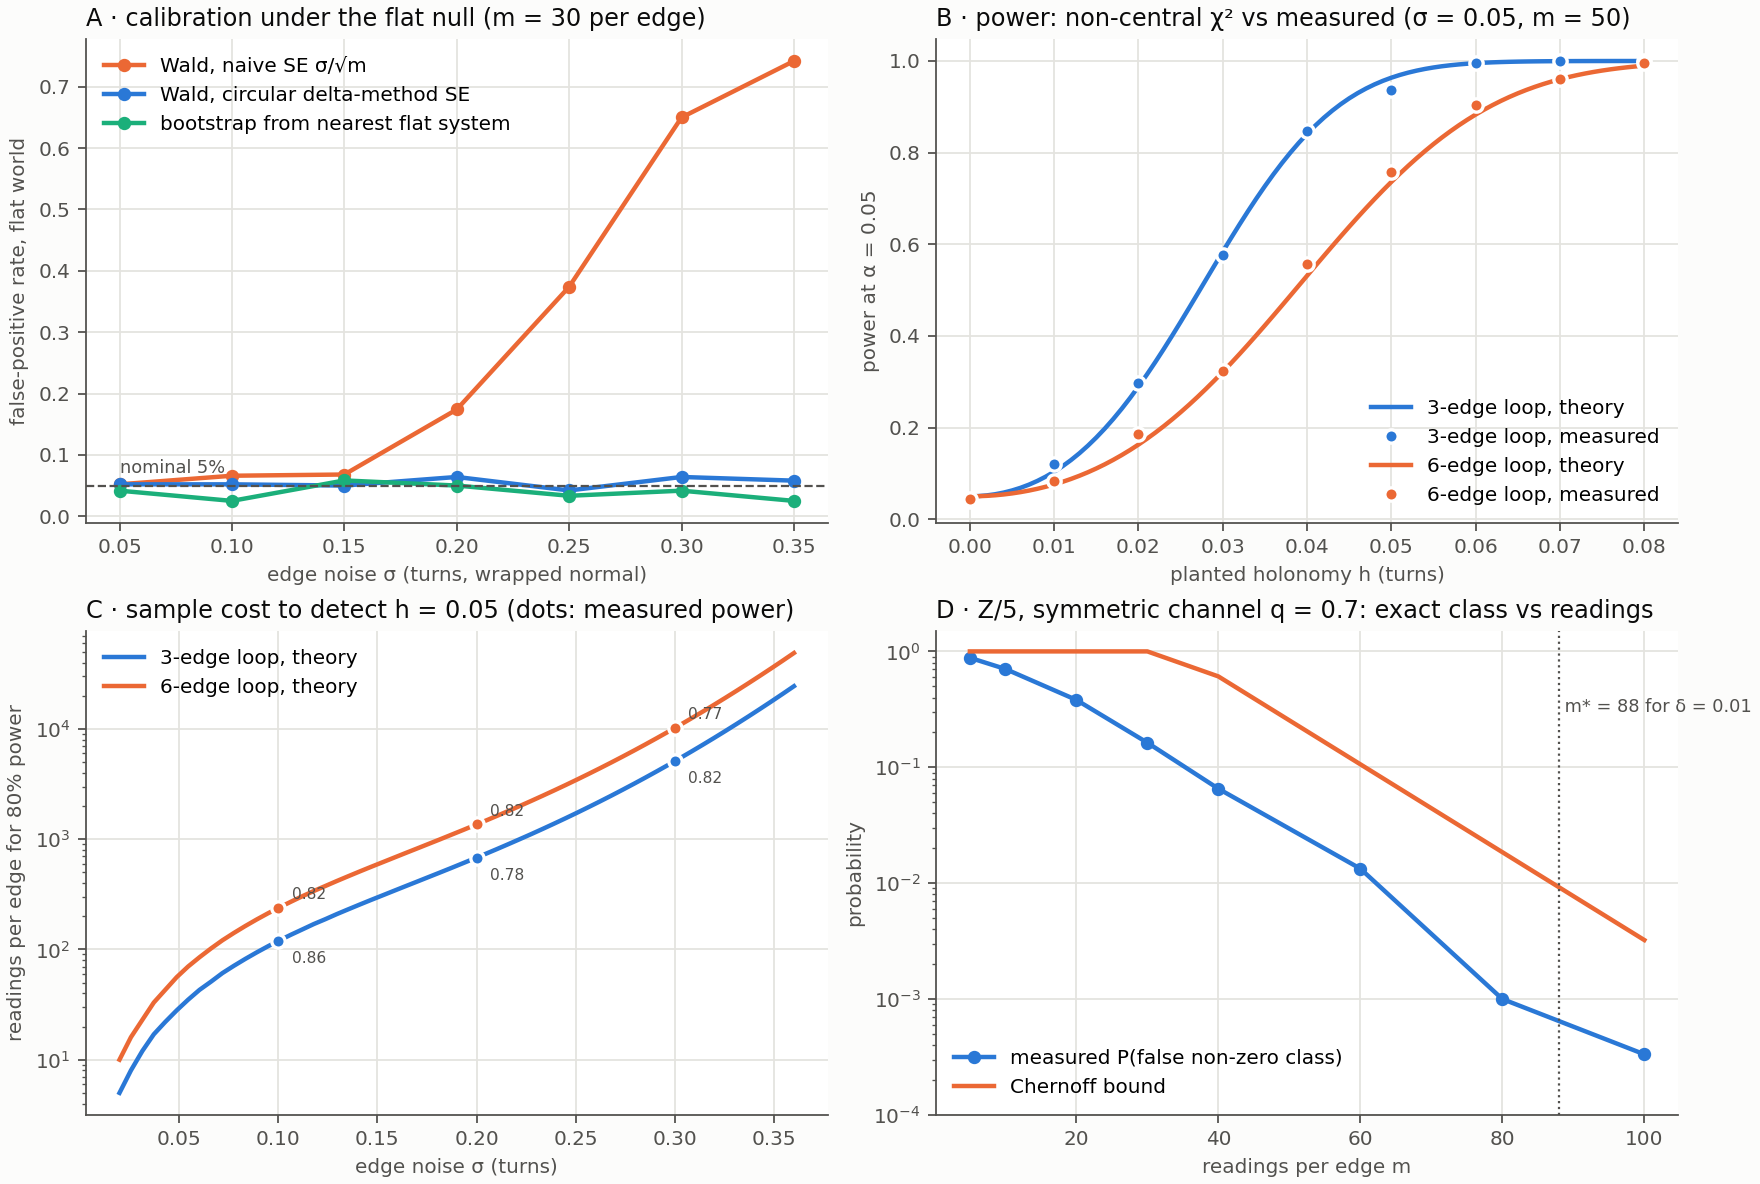
\includegraphics[width=\linewidth]{holonomy.png}
\caption{Problem 26 \src{S}. (A) calibration; (B) power against theory; (C) sample cost; (D) discrete class error against the Chernoff bound.}\end{figure}

%---------------------------------------------------------------------
\section{From operations to outcomes, around the probability layer}
\begin{theorem}[The operation-system model $e_g$]\label{thm:eg}\st{proved, computed}
For $(\Gamma,\Z/n,g)$, let the measurements be the vertex colours, the contexts the edges, and let $e_{ab}$ be uniform on $\{(x,x+g_{ab})\}$. Then:
\begin{enumerate}
  \item $e_g$ is strongly contextual iff $[g]\ne0$;
  \item for $[g]\ne0$, $\gamma(s)\ne0$ for every section over every nonzero coefficient ring;
  \item $e_g$ is an instance of an all-versus-nothing model over $\Z/n$ \cite{abklm15}.
\end{enumerate}
\end{theorem}
\begin{proof}
(1) A global section is exactly a global field.

(2) Take a compatible $R$-family with $r_{C_0}=s$. Its restrictions to vertices are functions $f_v:\Z/n\to R$. Each support is the graph of a bijection, so compatibility forces $f_b(y)=f_a(y-g_{ab})$. Propagating the delta function $f=\delta_{x_0}$ from $C_0$ around a loop with $h\ne0$ gives $\delta_{x_0}=\delta_{x_0+h}$, which is impossible when $R\ne0$.
\end{proof}
\begin{proposition}[Layer 2 is blind to {$[g]$}]\label{prop:blind-eg}\st{proved}
In $e_g$, every edge has $I(c_a;c_b)=\log n$ whatever $g$ is. More generally, any per-context functional invariant under relabelling outcomes (every Shannon or Tsallis functional) is unchanged by post-composing an edge with a permutation.
\end{proposition}
\noindent The ring-invariance in Theorem~\ref{thm:eg}(2) contrasts with the mod-3 grid, where $\gamma$ vanishes over $\Q$. Ring dependence of $\gamma$ is a property of the family, not of $\gamma$.

%---------------------------------------------------------------------
\section{Lossy operations}
Each edge carries a doubly stochastic channel $K$. Colours are uniform, so the Bayesian inverse is $K^\top$. The loop operator $M_L$ is the product around the loop, and the edge-context model $e_K$ has law $\tfrac1nK_{ab}$ on edge $(a,b)$.

\begin{proposition}[Character eigenvalues]\label{prop:eig}\st{proved}
For covariant channels $C_{\mu_e}S_{g_e}$ on a finite abelian $A$, every character $\chi$ is an eigenvector of $M_L$ with $\lambda_\chi=\big(\prod_e\hat\mu_e(\chi)\big)\chi(h)$. For the noisy shift $K=(1-\varepsilon)S_g+\varepsilon U$, $M_L=(1-\varepsilon)^{|L|}S_h+[1-(1-\varepsilon)^{|L|}]U$ and $\lambda_\chi=(1-\varepsilon)^{|L|}\chi(h)$.
\end{proposition}
\begin{corollary}
The labelled eigenvalue is base-point free, and its phase is $\chi(h)$ when every $\hat\mu_e(\chi)$ is real and positive. The unlabelled multiset is base-point free for \emph{any} channels, since $AB$ and $BA$ share their nonzero spectrum, but on $\Z/p$ it sees only the order of $h$. Asymmetric noise adds its own phase: the readout is $2.285$ instead of $2$.
\end{corollary}
\begin{proposition}[Information closed forms]\st{proved}
$I(c_a;c_b)=\log_2n+(1-\varepsilon+\tfrac\varepsilon n)\log_2(1-\varepsilon+\tfrac\varepsilon n)+(n-1)\tfrac\varepsilon n\log_2\tfrac\varepsilon n$. The loop-composite information is the same with $\varepsilon_L=1-(1-\varepsilon)^{|L|}$. Both are independent of $h$.
\end{proposition}

\begin{theorem}[Contextual fraction on a cycle]\label{thm:cfcycle}\st{proved}
On a cycle of length $L$ with noisy shifts and holonomy $h\ne0$ in a finite abelian $A$,
\[
\CF(e_K)=\max\!\Big(0,1-\frac{L\varepsilon}{2}\Big),
\]
independent of $|A|$ and of $h$.
\end{theorem}
\begin{proof}
\emph{Upper bound on NCF.} Weight each cell by its discrepancy $d=y-x-g$: $w(0)=0$, $w(-h)=1$, and $w=\tfrac12$ otherwise. Discrepancies sum to $-h\ne0$, so every colouring has weight at least 1. The dual value is $L\tfrac\varepsilon n(1+\tfrac{n-2}2)=\tfrac{L\varepsilon}2$.

\emph{Lower bound (packing).} Take colourings with one violation of discrepancy $-h$ (mass $\varepsilon/n$ per edge), and colourings with two violations $(a,-h-a)$ (mass $\varepsilon/(2n(L-1))$ per ordered edge pair), spread over translations. These fill every off-graph class exactly, and the on-graph load $\tfrac{L\varepsilon}2-\varepsilon(1-\tfrac1n)$ fits within the capacity $1-\varepsilon(1-\tfrac1n)$ iff $L\varepsilon\le2$.

\emph{Beyond the threshold.} The model is affine in $\varepsilon$ and non-contextual at $\varepsilon=2/L$ and at $\varepsilon=1$.
\end{proof}
\begin{theorem}[Any graph, lower bound]\label{thm:girth}\st{proved}
$\CF(e_K)\ge\max(0,1-\lmin\varepsilon/2)$, where $\lmin$ is the shortest simple cycle with nonzero holonomy.
\end{theorem}
\begin{observation}\st{measured}
Equality holds in 44 configurations: $\theta$-graphs, $K_4$, shared edges, shared vertices, disjoint non-flat loops, and $\varepsilon\le0.8$. Only $\lmin$ matters, not the cycle basis. The general packing is \st{open}.
\end{observation}
\begin{counterexample}[What does not hold]\label{ce:info}\st{computed}
\begin{itemize}
  \item \emph{Information does not determine CF.} A 3-cycle and a 5-cycle over $\Z/3$ at $\varepsilon=0.2$ have the same per-edge information, but $\CF=0.70$ and $0.50$.
  \item \emph{Non-covariant noise is contextual on its own.} Flat systems reach $\CF$ up to $0.24$, and the phase readout of $h=2$ spreads over $[1.1,3.1]$.
  \item \emph{Entropy is not a function of Fourier moduli.} A homometric pair has identical $|\hat p|$ but $H=2.7714$ against $2.7689$ bits.
\end{itemize}
\end{counterexample}

\begin{table}[h]\centering\small
\begin{tabular}{llll}
\toprule
layer & invariant & response to $\varepsilon$ & detects $h$ until\\
\midrule
1 & labelled eigenvalue of $M_L$ & modulus $(1-\varepsilon)^{|L|}$, phase fixed & $\varepsilon\to1$\\
2 & per-edge and loop $I$ & decreases, independent of $h$ & never\\
3 & $\CF$ & $1-\lmin\varepsilon/2$ & $\varepsilon=2/\lmin$\\
3 & $\gamma$ & support becomes full & $\varepsilon=0$ only\\
\bottomrule
\end{tabular}
\caption{The same noise acting on four invariants \src{S}.}
\end{table}

\begin{figure}[h]\centering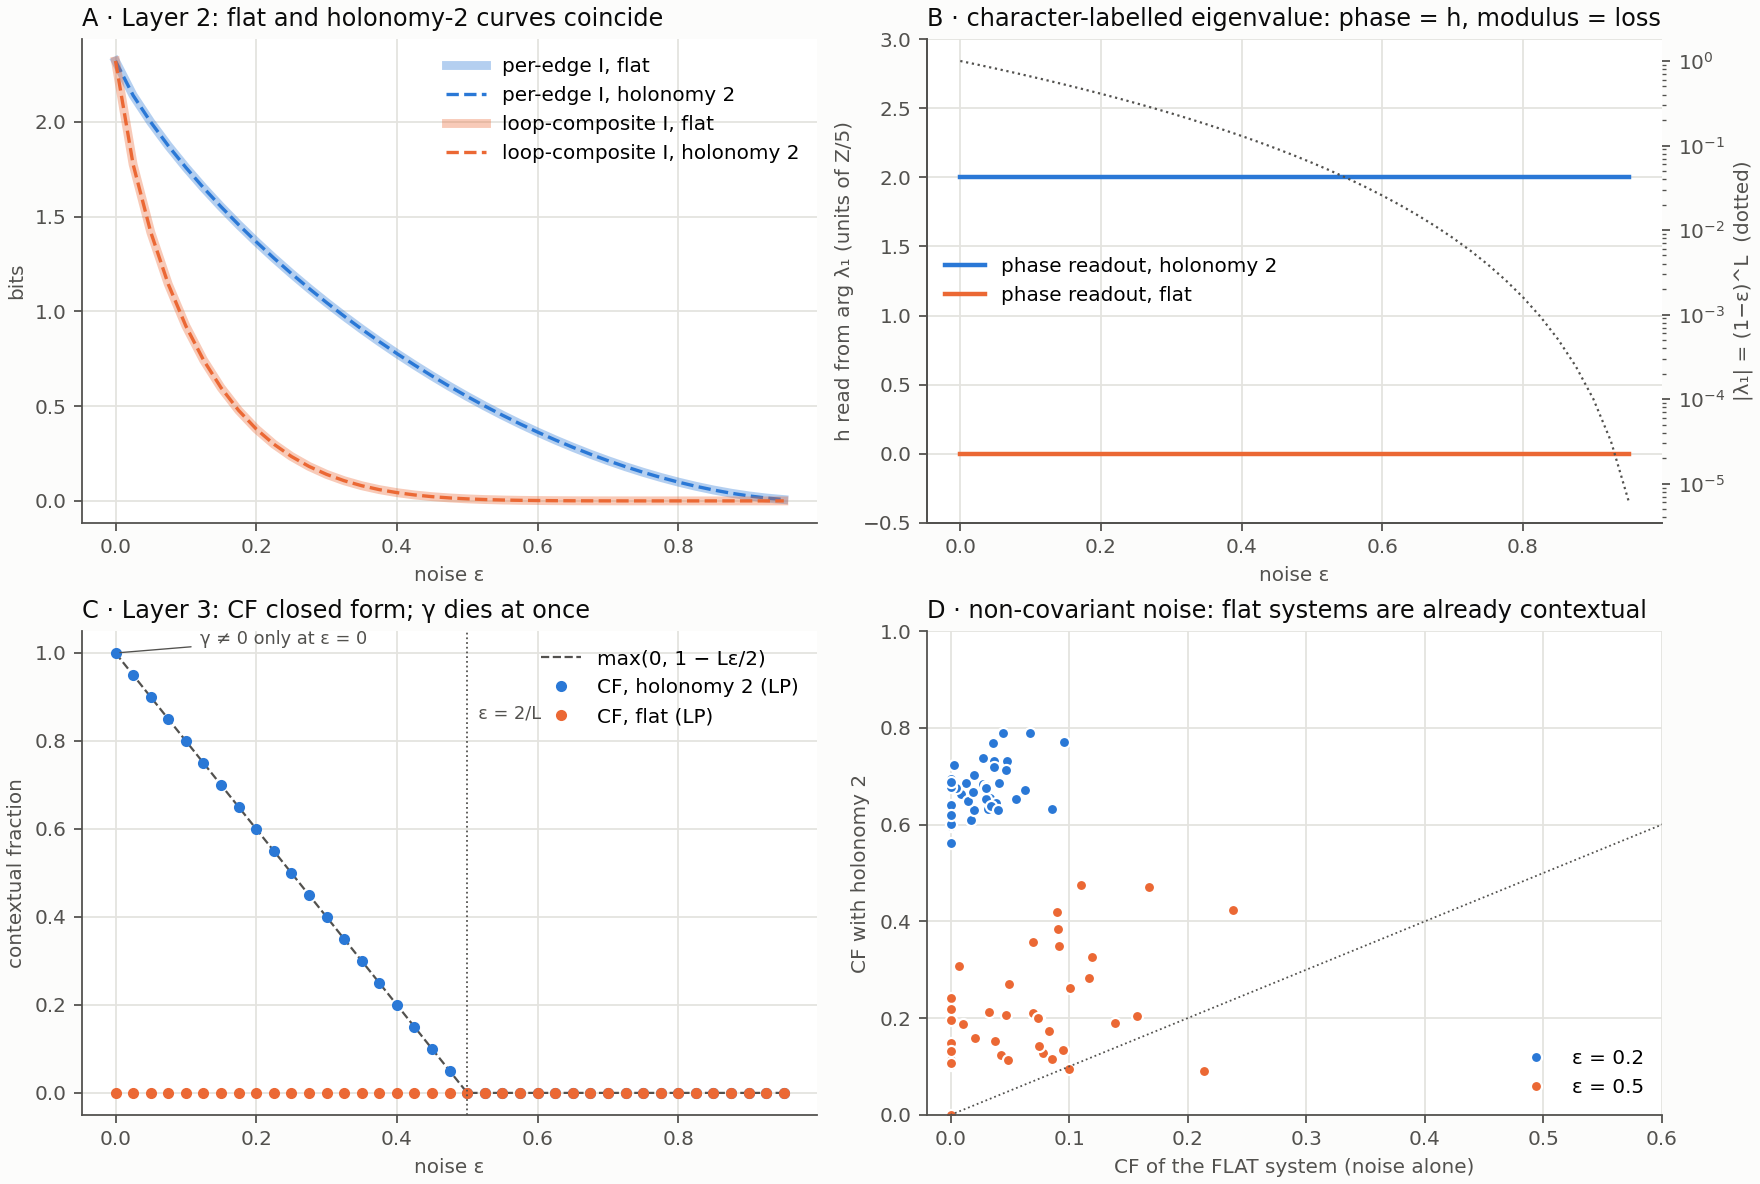
\includegraphics[width=\linewidth]{channels.png}
\caption{Noisy operations on a 4-cycle over $\Z/5$, with $h=2$ against a flat system \src{S}.}\end{figure}

\begin{proposition}[Orientation for $\Z/3$ and $\Z/5$]\st{proved, computed}
For odd primes, $h\ne-h$ whenever $h\ne0$, so the labelled phase always detects orientation. Reversing the loop inverts the readout ($1\leftrightarrow4$ and $2\leftrightarrow3$ on $\Z/5$). The unlabelled multiset and $\CF$ do not detect orientation.
\begin{itemize}
  \item On $\Z/3$ a non-flat holonomy is exactly a chirality, read from the sign of $\operatorname{Im}\lambda_1$.
  \item On $\Z/5$ the phase splits into a magnitude class, $\operatorname{Re}\lambda_1/|\lambda_1|=0.309$ for $\pm1$ and $-0.809$ for $\pm2$, and an orientation.
  \item The magnitude class is meaningful only with fixed state labels, since $x\mapsto2x$ carries $h=1$ to $h=2$.
\end{itemize}
\end{proposition}

%---------------------------------------------------------------------
\section{The support dial: Tsallis entropies}\label{sec:tsallis}
\begin{proposition}\st{computed; the cocycle property is Vigneaux's}
Let $S_\alpha=(1-\sum p^\alpha)/(\alpha-1)$ with the deformed action $(X\cdot_\alpha F)(P)=\sum_xP(X{=}x)^\alpha F(P\mid X{=}x)$.
\begin{itemize}
  \item $S_\alpha$ is a $\delta_\alpha$-cocycle (defect below $3\times10^{-15}$), but not a cocycle for Shannon's action (defect up to $1.8$).
  \item $S_0=|\mathrm{supp}|-1$, and $S_\alpha\to H$ as $\alpha\to1$.
  \item Mass $\epsilon$ added to an empty cell changes $S_0$ by 1, and $S_\alpha$ by $\sim\epsilon^\alpha$.
  \item $S(X)+S(Y)-S(XY)$ reaches $-1.71$ at $\alpha=0.5$.
\end{itemize}
$\alpha$ therefore interpolates between AMB's possibilistic lens ($\alpha=0$) and Shannon ($\alpha=1$). Every $S_\alpha$ is symmetric, so Proposition~\ref{prop:blind-eg} still holds.
\end{proposition}

%---------------------------------------------------------------------
\section{Support strata: where each lens can see anything}\label{sec:strata}
An empirical model $e=(e_C)_C$ lies in a product of simplices $\prod_C\Delta(O^C)$, intersected with the no-signalling polytope. Its \emph{support} is $\sigma(e)=(\operatorname{supp}e_C)_C$. The \emph{stratum} of $e$ is the set of models with the same support, that is, the relative interior of a face.
\begin{itemize}
  \item The \emph{interior} is full support in every context.
  \item The \emph{vertices} are one outcome per context.
\end{itemize}

\begin{proposition}[Support stratification]\label{prop:strata}\src{S}\st{proved}
\begin{enumerate}
  \item \emph{Face functions.} The support presheaf $\mathcal S_e$, its global sections, logical and strong contextuality, and $\gamma$ over every ring depend on $e$ only through $\sigma(e)$. Strong contextuality is inherited by smaller supports: if $\sigma(e)\subseteq\sigma(e')$ componentwise and $e'$ is strongly contextual, so is $e$.
  \item \emph{Interior.} With full support, every local section extends to a global section of $\mathcal S_e$. So $e$ is not logically contextual and $\gamma(s)=0$ for every $s$, over every ring. The contextual fraction can still be positive.
  \item \emph{Vertices.} If each $e_C=\delta_{s_C}$ and $e$ is no-signalling on a cover of the measurements, the $s_C$ glue to a global assignment $g$ with $e=\delta_g|_{\mathcal C}$. Then:
  \begin{itemize}
    \item $e$ is non-contextual, $\CF=0$ and $\gamma=0$;
    \item every Shannon and Tsallis functional of every context vanishes, together with every mutual and conditional information, since each is a combination of entropies of point masses.
  \end{itemize}
  \item \emph{The probability lens varies within strata.} $\CF$ is not a face function. It is convex (Abramsky--Barbosa--Mansfield), hence continuous on the relative interior of the model polytope. $S_\alpha$ for $\alpha>0$ and $H$ are continuous on closed simplices. $S_0=|\operatorname{supp}|-1$ is constant on strata and jumps exactly across them.
\end{enumerate}
\end{proposition}
\begin{proof}
\begin{enumerate}
  \item $\mathcal S_e(U)$ is the set of sections over $U$ whose restrictions to each context lie in $\operatorname{supp}e_C$. Every listed invariant is defined from $\mathcal S_e$. If $\sigma(e)\subseteq\sigma(e')$ then $\mathcal S_e\subseteq\mathcal S_{e'}$, so a global section of $\mathcal S_e$ is one of $\mathcal S_{e'}$.
  \item Extend $s\in O^C$ arbitrarily to $g\in O^X$. Every restriction of $g$ lies in a full support, so $g\in\mathcal S_e(X)$. A section that extends to a global section has trivial obstruction and is no logical witness.
  \item No-signalling gives $\delta_{s_C}|_{C\cap C'}=\delta_{s_{C'}}|_{C\cap C'}$, so $s_C|_{C\cap C'}=s_{C'}|_{C\cap C'}$. Because the contexts cover $X$, the $s_C$ glue to a unique $g$, and $\delta_g$ is a global law. $H(\delta)=S_\alpha(\delta)=0$ for all $\alpha$.
  \item The Tsirelson box and white noise lie in the same (interior) stratum, with $\CF=0.414$ and $0$. Continuity of $S_\alpha$ for $\alpha>0$ and the jump of $S_0$ are immediate from the formulas.
\end{enumerate}
\end{proof}

\begin{corollary}\st{proved}
A nonzero $\gamma$ and logical contextuality occur only on \emph{intermediate} strata: neither full support nor single outcomes.
\begin{itemize}
  \item The PR box has no global section and 8 cohomological witnesses.
  \item The Hardy model has one logical witness, missed by $\gamma$ over $\Z$.
\end{itemize}
Contextuality in the interior is visible only to the probability lens ($\CF$); the possibilistic lens is blind to it. $S_0$ reads the stratum and $S_{\alpha>0}$ reads the position within it, which completes the support dial of Section~\ref{sec:tsallis}.
\end{corollary}

\begin{proposition}[Two-outcome supports are all-or-nothing]\label{prop:two}\src{S}\st{proved}
Consider a graph scenario with binary measurements and pairwise contexts. Let $e$ be no-signalling with $|\operatorname{supp}e_C|=2$ for every context.
\begin{enumerate}
  \item Every measurement is either \emph{pinned} (deterministic) or \emph{free} (both values occur). An edge between two free measurements has a bijection support $\{y=x+c_C\}$ with $c_C\in\Z/2$. An edge between a pinned and a free measurement has a product support. No edge joins two pinned measurements.
  \item $e$ is contextual if and only if the $\Z/2$ connection $c$ on the free subgraph has a non-flat cycle. It is then \emph{strongly} contextual, with $\CF=1$ and $\gamma\neq0$. Otherwise every local section extends and $\gamma=0$. Logical-but-not-strong contextuality, as in Hardy, needs a support of size at least 3.
  \item On a component with a non-flat cycle, no-signalling forces every free marginal to be $\tfrac12$, so the stratum is a single point there. On a flat component the stratum is a one-parameter family $q\in(0,1)$ with $\CF=0$.
  \item Per context, $H=I=h(q)$ and $S_0=1$. The non-flat point and the flat point $q=\tfrac12$ have identical per-context Shannon and Tsallis profiles, yet $\CF=1$ and $0$.
\end{enumerate}
\end{proposition}
\begin{proof}
\begin{enumerate}
  \item A size-2 subset of $\{0,1\}^2$ either fixes one coordinate or is the graph of a bijection. No-signalling makes pinned/free a property of the measurement.
  \item Global sections are the pinned values together with a flat section of the $\Z/2$ torsor on the free subgraph, which exists if and only if every cycle is flat. If no flat section exists, then $\mathcal S_e(X)=\emptyset$, and $\CF=1$ by Abramsky--Barbosa--Mansfield. If one exists, a torsor section is fixed by any one value on each component, so every local section extends.
  \item A bijection edge transports the marginal $p\mapsto p$ or $p\mapsto1-p$, and an odd cycle gives $p=1-p$.
  \item The joint on a bijection edge is determined by its marginal. Relabelling invariance gives the last claim, which is Proposition~\ref{prop:blind-eg} at $n=2$.
\end{enumerate}
\end{proof}
\noindent So at two outcomes, Layer~3 is exactly $\Z/2$ holonomy. The information lens sees only the free parameter $q$, and $q$ is pinned to $\tfrac12$ precisely when the holonomy is non-trivial.

\noindent\emph{Checked:} the CHSH parity family (\texttt{test\_two\_outcome\_supports\_all\_or\_nothing}):
\begin{itemize}
  \item flat models are non-contextual for $q=0.5,0.7,0.9$;
  \item the odd model at $q=0.9$ signals (defect $0.8$);
  \item at $q=\tfrac12$ the odd model is the PR box, with $\CF=1$ and a profile identical to the flat model's.
\end{itemize}

\begin{remark}[What this replaces]\st{withdrawn}
A proposed ``sheaf--geometric bridge'' identified $\gamma_{\mathrm{AMB}}$ with the boundary holonomy of a smooth circle bundle through a support-reduction functor $\chi$. It placed contextuality at single-outcome supports and tied it to the divergence of $\partial H/\partial p_i$ at $\partial\Delta$. It is rejected here, for four reasons:
\begin{itemize}
  \item Its central equation equates an integer class taken mod $\Z$, which is $0$, with a holonomy that is never defined.
  \item The AMB cover is a finite cover of a measurement set, not an open cover of a manifold, and $\chi$ is never constructed.
  \item Information cohomology uses measurable cochains and functional equations, so the divergence of a derivative cannot create a class. Its $H^{\ge2}$ is open, and ``$I=dH$'' conflates de Rham $d$ with $\delta$ and $\delta_t$ (we have $I=\delta_tH$).
  \item By Proposition~\ref{prop:strata}(3), single-outcome models are exactly where both lenses vanish.
\end{itemize}
The correct discrete statement relating holonomy and $\gamma$ is the connecting-class result for operation systems (Theorem~\ref{thm:eg}). The correct role of the simplex boundary is the stratification above.
\end{remark}
\noindent Checked in \texttt{tests/test\_strata.py}: interior (Tsirelson, noisy PR, noisy GHZ); vertices (random deterministic assignments on the CHSH, GHZ and $\Z/3$ grid scenarios); a CF-versus-face counterexample; and the intermediate faces.

%---------------------------------------------------------------------
\section{Magnitude and phase: what Layer 2 reads}\label{sec:magphase}
Proposition~\ref{prop:blind-eg} cannot be evaded by choosing a different symmetric functional. This section says what Layer~2 \emph{does} read, and how little must be added to recover $\CF$.

\begin{proposition}[Logical Bell bound]\label{prop:lbell}\src{S}\st{proved}
Let $\varphi_1,\dots,\varphi_n$ be formulas on contexts $C_1,\dots,C_n$ that are jointly unsatisfiable, as in Abramsky \cite{abramsky20}, and let $p_i=e_{C_i}(\varphi_i)$. Then $\CF(e)\ge\sum_ip_i-(n-1)$.
\end{proposition}
\begin{proof}
Write $e=(1-\lambda)e^{NC}+\lambda e'$ with $\lambda=\CF(e)$. A global assignment satisfies at most $n-1$ of the $\varphi_i$, so the non-contextual part contributes at most $n-1$ to $\sum_i p_i$, and the rest contributes at most $n$. Hence $\sum_ip_i\le(1-\lambda)(n-1)+\lambda n$.
\end{proof}
\noindent The bound costs linear time. A Liar cycle ($x_1=x_2,\dots,x_n=\neg x_1$) is the case of odd $\Z/2$ holonomy. For $n=4$ it is the PR box \cite{abramsky20}, which is Proposition~\ref{prop:two}.

\begin{proposition}[$\CF$ from moduli and one bit]\label{prop:modphase}\src{S}\st{lower bound proved; equality computed for $n=3,\dots,6$}
Take a binary $n$-cycle with uniform marginals and edge correlations $s_i=\mathbb E[(-1)^{a+b}]$.
\begin{enumerate}
  \item Layer~2 determines each modulus $|s_i|$ and nothing else about the $s_i$. The Shannon form is $I_i=\log2-h\bigl(\tfrac{1+|s_i|}2\bigr)$. The Tsallis-2 form, with Vigneaux's action, is $I_{2,i}=S_2(b)-a\cdot_2S_2(b)=(1+s_i^2)/4$. The signs are invisible by Proposition~\ref{prop:blind-eg}, and their product is the holonomy bit.
  \item The contextual fraction is
  \[
  \CF=\begin{cases}\max\bigl(0,\tfrac12(\sum_i|s_i|-(n-2))\bigr) & \text{odd holonomy,}\\[2pt]
  \max\bigl(0,\tfrac12(\sum_i|s_i|-2\min_i|s_i|-(n-2))\bigr) & \text{flat.}\end{cases}
  \]
  The right-hand side is a lower bound by Proposition~\ref{prop:lbell}, applied to the odd sign pattern that is best aligned with the $s_i$. Equality is computed for $n=4$: the LP agrees to $10^{-15}$ on 60 random models in \texttt{tests/test\_magnitude\_phase.py}, and on 300 in an exploratory run. For $n=3,4,5,6$ it agrees to $4\cdot10^{-16}$ on 160 random cycles (\texttt{tests/test\_weak\_edge.py}).
\end{enumerate}
\end{proposition}
\noindent\emph{Consequences.}
\begin{itemize}
  \item The holonomy bit moves $\CF$ by at most $\min_i|s_i|$. On 300 random CHSH models it moved $\CF$ by $0.078$ on average and by $0.82$ at most. With a noisy edge, Layer~2 alone nearly determines $\CF$.
  \item A flat cycle with one uniform edge ($|s_j|=0$) and the other edges perfect has $\CF=\tfrac12$.
  \item The Tsallis-2 form needs no inverse entropy: $|s_i|=\sqrt{4I_{2,i}-1}$. Independent bits give $I_2=\tfrac14$, not $0$, which is non-additivity. $S_2$ also has an exactly unbiased estimator, $\sum_xn_x(n_x-1)/N(N-1)$, so it avoids the Miller--Madow bias of plug-in Shannon estimates.
\end{itemize}

\begin{remark}[Grassmannian charts: magnitude is chart-invariant, phase is the chart coordinate]\label{rem:grass}\st{proved (identities); interpretation}
\begin{itemize}
  \item \emph{Exponential charts.} $\operatorname{Gr}(k,n)=GL_n/P$ has big cell $\exp(\mathfrak n^-)P$ with $\mathfrak n^-\cong\operatorname{Hom}(\F^k,\F^{n-k})$. For Grassmannians $\mathfrak n^-$ is abelian with $X^2=0$, so $\exp X=I+X$ and the chart $X\mapsto\operatorname{row}[I\mid X]$ is linear.
  \item \emph{Point counts.} Over $\F_q$, $|\operatorname{Gr}(k,n)|=\sum_\lambda q^{|\lambda|}=q^{k(n-k)}(1+O(q^{-1}))$.
  \item \emph{$S_2$ is a dimension.} For flags of type $k=(k_1,\dots,k_s)$,
  \[
  \dim\operatorname{Flag}(k)=\sum_{i<j}k_ik_j=\tfrac12\Bigl(n^2-\sum_ik_i^2\Bigr),\qquad\text{so}\qquad S_2(k/n)=\frac{2}{n^2}\dim\operatorname{Flag}(k)
  \]
  exactly. This underlies Vigneaux's limit $\tfrac{2}{n^2}\log_q\binom{n}{pn}_q\to S_2(p)$ \cite{vig}. Shannon entropy is the log of a set count, the multinomial, and $q\to1$ recovers it.
  \item \emph{Edges as chart points.} For the operation systems over $\F_p^k$, the support of edge $e$ is the graph of $G_e$, the point $\operatorname{row}[I\mid G_e]\in\operatorname{Gr}(k,2k)$. \emph{Its exponential coordinate is the operation $G_e$.} Affine maps are homogenised to $\F_p^{k+1}$.
  \item \emph{Two lenses.}
  \begin{itemize}
    \item Holonomy is the product of coordinates around a loop. The space of global sections has dimension reduced by $\operatorname{rank}(G_{\text{loop}}-I)$; for a translation by $h\neq0$ the loop matrix $\bigl(\begin{smallmatrix}1&h\\0&1\end{smallmatrix}\bigr)$ fixes 1 of 2 dimensions.
    \item Dimension, $S_2$ and entropy are $GL$-invariant, hence the same in every chart. That is Layer~2's blindness in geometric form.
    \item Chart invariants read magnitude (Layer 2). Coordinates composed around loops read phase (Layer 3).
  \end{itemize}
  \item \emph{Global structure.} No single chart covers $\operatorname{Gr}(k,n)$, and the transitions are non-linear (Pl\"ucker). The global invariants, Schubert classes and tautological Chern classes, live in the gluing, just as holonomy does.
\end{itemize}
\emph{Not claimed.} Vigneaux proves that differential entropy and dimension are the only degree-1 classes for Gaussian modules without coordinates. Whether dimension is a cocycle in a finite-field information structure built from our operation systems is settled in Proposition~\ref{prop:ffdim} below.
\end{remark}

\begin{proposition}[Dimension over $\F_p$]\label{prop:ffdim}\src{S}\st{proved; computed}
Laws on $\F_p^n$ whose support is an affine subspace form a sub-functor: it is closed under linear pushforward and under conditioning on a linear observable. On it, $D[X](P)=\log_p|\operatorname{supp}X_*P|$ is a 1-cocycle for the Shannon action,
\[
D[XY]=D[X]+\textstyle\sum_xP(x)\,D[Y](P\mid X=x).
\]
The reason is that every fibre $A\cap X^{-1}(x)$ is a coset of $A\cap\ker X$, so all fibres have the same dimension. On general laws the identity fails (defect up to $0.42$). The count $S_0=|\operatorname{supp}|-1$ is a cocycle for the $\alpha=0$ action on all laws.
\end{proposition}
\noindent\emph{Computed} (\texttt{magphase.py}, \texttt{tests/test\_magphase\_module.py}): 300 random affine-support laws on $\F_3^3$ with random linear observables give defect $\le7\times10^{-16}$; general laws give up to $0.42$.

\noindent\emph{Consequence.} Dimension is a Layer-2 cocycle in our finite-field setting, on affine supports. Its non-triviality would follow from the Baudot--Bennequin locality convention (local 0-cochains are constants), which we have not checked separately. Per edge it is constant, $D=1$ for every graph of a bijection of $\F_p$, so it is blind to holonomy, as Proposition~\ref{prop:blind-eg} requires. Holonomy appears only in the dimension of the \emph{glued} section space.

\paragraph{Dimension deficit from estimated supports.}\src{S}\st{measured}
Setup (\texttt{examples/dimension\_deficit.py}):
\begin{itemize}
  \item a 4-cycle over $\F_3$ and $\F_5$, with $N\in\{30,90,300\}$ samples per edge and symmetric noise $\varepsilon\in\{0.1,0.3\}$;
  \item edge supports thresholded at $\tau\in[0.2,0.6]$, and an edge accepted only if its support is the graph of an affine bijection;
  \item the loop map in homogeneous coordinates, and the statistic $\operatorname{rank}_{\F_p}(M_{\text{loop}}-I)$;
  \item a null band from a parametric bootstrap under the nearest flat system.
\end{itemize}
Three systems are planted:
\begin{itemize}
  \item \emph{flat}: deficit 0, $p$ global sections;
  \item \emph{translation holonomy}: deficit 1, 0 global sections, strongly contextual;
  \item \emph{multiplicative holonomy} ($a_{\text{loop}}=2$): deficit 1, exactly 1 global section (the fixed point), logically but not strongly contextual.
\end{itemize}
Findings:
\begin{itemize}
  \item Whenever all supports were recovered, the deficit was correct in every replicate. The null band was 0 at every $(\varepsilon,N,\tau)$.
  \item The statistic fails by \emph{abstaining}: at $\F_5$, $\varepsilon=0.3$, $N=30$, recovery is 2--9\%.
  \item $\gamma$ over $\Z$ and over $\Z/p$ agrees with the deficit in all six cases. The holonomy test covers only translations.
  \item The global-section count separates strong from logical contextuality, which the deficit alone does not.
\end{itemize}
\emph{Scope.} Under symmetric noise a failed recovery is a non-bijection, never a wrong bijection, so the null band is trivially 0. Non-covariant noise could produce wrong bijections and is untested.

\paragraph{Estimation: $S_2$ versus Shannon.}\src{S}\st{measured}
Moduli $|s_i|$ and $\CF$ of a binary 4-cycle were estimated from $N$ samples per edge, with 400 replicates for each of three configurations (\texttt{examples/s2\_vs\_shannon.py}). Four estimators were compared: unbiased $I_2$, Shannon plug-in, Miller--Madow, and the labelled sample correlation.
\begin{itemize}
  \item At $N\ge100$ all four agree to within $0.003$ in RMSE of $\CF$.
  \item At $N=30$ the $S_2$ route has the smallest bias in $s^2$ on weak edges ($0.017$ against $0.035$). It has the \emph{largest} $\CF$ RMSE on strong and near-threshold edges ($0.087$ against $0.067$, and $0.153$ against $0.125$), because $\CF$ needs $|s|=\sqrt{s^2}$ clipped to $[0,1]$.
  \item \emph{$S_2$ does not pay off here.} With uniform marginals, each $2\times2$ table has a one-dimensional sufficient statistic, the agreement count. Every lens is then a function of it, and unbiasedness of $s^2$ does not carry through the square root.
\end{itemize}

%---------------------------------------------------------------------
\section{A contradiction meter with provenance}\label{sec:meter}
\textbf{Input.} A claim $(u,i,j,r)$ means that provenance unit $u$ (a source, document or turn) asserts $x_i\oplus x_j=r$ about binary propositions. Claims may be single assertions (deterministic mode) or repeated samples.

\textbf{Three separate failures} \src{S}:
\begin{enumerate}
  \item \emph{Self-contradiction}: an odd cycle among one unit's own claims.
  \item \emph{Overlap disagreement} ($d^0\neq0$, the deficit): two units give the same edge different parities, significant at $z>3$ in sampled mode. It is recorded and the edge is \emph{not} glued.
  \item \emph{Contextuality across provenance} ($d^0=0$, $H^1\neq0$): the overlaps agree, but the glued graph has an odd cycle contained in no single unit. This is a Liar cycle (Proposition~\ref{prop:two}).
\end{enumerate}
Each cycle is reported with:
\begin{itemize}
  \item the logical-Bell lower bound on $\CF$ (Proposition~\ref{prop:lbell});
  \item a union-bound confidence that all of its parities are right;
  \item a blamed edge, only when every other edge comes from a declared trusted unit.
\end{itemize}
Coherent fabrications are invisible by construction.

\textbf{v1 changes} \src{S}:
\begin{enumerate}
  \item \emph{Pooled noise.} The flip rate $\hat\varepsilon$ is estimated by EM over all claims, with each edge's true parity latent. An edge's error probability is then the posterior $\lambda^{d}/(1+\lambda^{d})$, where $\lambda=\hat\varepsilon/(1-\hat\varepsilon)$ and $d$ is the majority margin. This replaces the worst-case binomial.
  \item \emph{Shortest odd cycles.} For every edge, the meter finds the shortest odd cycle through it by BFS in the parity double cover. It replaces fundamental cycles.
  \item \emph{Multiple testing.} Cycles are certified at level $\alpha/k$ over the $k$ candidates (Bonferroni).
\end{enumerate}

\textbf{Benchmark} \st{measured} (\texttt{examples/meter\_benchmark.py}).
\begin{itemize}
  \item \emph{Data}: 12 propositions and 4 honest units asserting 6 true parities each, with one added unit per scenario; 200 instances per cell. Results are in Table~\ref{tab:meter}.
  \item \emph{Pooling}: it fixes the $m=5$ row. At $\varepsilon=0.1$, self-contradictions go from $0.00$ to $0.78$ and cross-unit cycles from $0.33$ to $0.84$.
  \item \emph{Clean cases}: honest-only firing stays at or below $0.04$, and coherent fabrications are not flagged.
  \item \emph{Limits}: at $\varepsilon=0.2$ with $m\le5$, power is low.
  \item \emph{Validation}: \texttt{tests/test\_meter.py} checks the CF lower bound against the LP on 3- and 5-cycles.
\end{itemize}
\begin{table}[h]\centering\small
\begin{tabular}{lccccc}
\toprule
$m$, $\varepsilon$, noise model & honest & self & overlap & cross (correct edge blamed) & fabrication\\
\midrule
1, 0 (deterministic) & 0.00 & 1.00 & 1.00 & 1.00 (1.00) & 0.00\\
5, 0.1, worst case & 0.00 & 0.00 & 0.74 & 0.33 (0.32) & 0.01\\
5, 0.1, pooled & 0.01 & 0.78 & 0.86 & 0.84 (0.84) & 0.01\\
3, 0.1, pooled & 0.04 & 0.37 & 0.61 & 0.55 (0.55) & 0.04\\
15, 0.2, pooled & 0.01 & 0.95 & 0.98 & 0.94 (0.94) & 0.00\\
5, 0.2, pooled & 0.04 & 0.21 & 0.56 & 0.19 (0.19) & 0.04\\
\bottomrule
\end{tabular}
\caption{Detection rates by planted scenario. The ``honest'' column is the false-positive rate of the full meter.}\label{tab:meter}
\end{table}

\paragraph{Relational claims: ``A said X'' and ``C caused D''.}\src{S}\st{measured} (\texttt{relclaims.py}, \texttt{examples/basil\_relational.py})
\textbf{Extraction.} Claims are extracted from spaCy dependency parses with transparent rules:
\begin{itemize}
  \item \emph{attribution}: a say-verb with a subject and a clausal complement, or ``according to''; deny, reject and dispute, or a negated verb, flip the polarity;
  \item \emph{causation}: cause, lead to, result in, trigger, spark, fuel, passive by-agents, and because of or due to; a negated verb flips the polarity.
\end{itemize}
\textbf{Stated axioms}:
\begin{itemize}
  \item A1: one statement has one speaker;
  \item A2: causation is not mutual;
  \item A3: there are no causal 3-cycles.
\end{itemize}
\textbf{Conflicts detected}:
\begin{itemize}
  \item \emph{polarity}: the same proposition asserted and denied;
  \item \emph{speaker}: A1 is violated;
  \item \emph{reversal}: A2 is violated;
  \item \emph{cycle}: A3 is violated by claims from two or more sources.
\end{itemize}
A speaker is used for A1 only when resolved. Role nouns, documents and channels (``the attorney'', ``the statement'', ``according to the Times'') are unresolved without coreference. Say-verbs nested in another say-verb's clause, and speakers inside quotations, belong to the outer speaker.

\textbf{Validation.} Ten planted mini-articles: one per conflict type, plus controls for a paraphrase, a causal chain, passive--active agreement, a role noun and a nested quote. All ten are classified correctly (\texttt{tests/test\_relclaims.py}).

\textbf{BASIL} (100 events, 3 outlets each).
\begin{itemize}
  \item \emph{Claims}: 1{,}667 attribution claims and 149 causal claims were extracted.
  \item \emph{Overlap}: only $43/1605$ attribution contents and $3/146$ causal pairs are made by two or more outlets in the same event. The opportunity to contradict is small, which is consistent with BASIL's finding that bias works through selection and framing.
  \item \emph{First pass}: 17 speaker flags, all reviewed by hand and none a contradiction. Thirteen were one person named two ways, two came from nested quotes, and two were different people saying similar lines.
  \item \emph{After resolution}: one flag, Lofgren against Pelosi on ``power grab''. These are two different quotes, and both can be true.
  \item \emph{Verdict}: no factual contradiction between outlets was found. The detector's value here is negative evidence, together with the overlap statistic. The rules are shallow, and recall on real text is unmeasured.
\end{itemize}

\paragraph{General binary claims.}\src{S}\st{proved (classification); computed}
Each unit's formulas define a local support $S_u\subseteq\{0,1\}^{C_u}$ (\texttt{meter\_general.py}; formula syntax: $\sim$, \&, $|$, $\hat{}$, $\to$, $\leftrightarrow$). A deletion-based minimal unsatisfiable set of units is classified as one of:
\begin{itemize}
  \item \emph{self}: $S_u=\emptyset$;
  \item \emph{overlap}: two units with disjoint projections onto their shared propositions;
  \item \emph{propagation}: arc consistency (semijoin reduction) empties a unit;
  \item \emph{cyclic}: arc consistency leaves every $S_u$ non-empty and consistent on overlaps ($d^0=0$), yet no global assignment exists.
\end{itemize}
By Beeri--Fagin--Maier--Yannakakis \cite{bfmy}, the cyclic type requires a cyclic hypergraph; this is the strongly contextual case. With assertion frequencies $p_u$, the core carries the logical-Bell bound $\CF\ge\sum p_u-(k-1)$.

\paragraph{Gaussian fast path over $\F_2$.}\src{S}\st{computed}
Weights of Gaussian type are closed under gluing, and gluing them is matrix algebra rather than a sum over assignments. The Grassmann--Gaussian weights of Korepanov and Sadykov \cite{korepanov}, whose 4-simplex weights are Grassmann--Gaussian exponents and whose Pachner-move relations are therefore algebraic identities between Gaussians, are an example of this principle; we use only this structural point, not their parameterisations. Over $\F_2$ the analogue is a unit whose support is an affine subspace, such as a parity, XOR or literal claim or a conjunction of these.
\begin{itemize}
  \item \emph{Method}: for such units, contradiction cores come from Gaussian elimination with row tracking. The combination $y$ with $yA=0$ and $yb=1$ is the certificate. A core is already minimal when $\operatorname{rank}=|\text{rows}|-1$ (a circuit); otherwise it is minimised by deletion.
  \item \emph{Timing}: brute force takes $0.35$\,s at 16 propositions and grows as $2^n$. The fast path handles a 5{,}000-claim Liar ring among 15{,}000 consistent distractor claims (20{,}000 propositions) in $0.66$\,s.
  \item \emph{Validation}: cores match brute force and are minimal on 40 random parity systems (\texttt{tests/test\_meter\_general.py}).
  \item \emph{Scope}: non-affine claims such as $A\to B$ keep the exact but exponential path. General satisfiability is NP-hard, and the $\CF$ LP is not reduced by this.
\end{itemize}

\paragraph{First real run: BASIL, overlap channel.}\src{S}\st{measured}
\textbf{Setup} (\texttt{examples/basil\_overlap.py}):
\begin{itemize}
  \item BASIL \cite{basil}: 97 events with all three outlets (Fox, NYT, HuffPost) annotated; gold annotations only.
  \item Sources are the outlets. A proposition is ``the article is negative toward target $T$ in event $t$''.
  \item Literals are encoded as parity edges to an anchor proposition, so cycles cannot arise and only the overlap channel is exercised.
  \item Null: outlet labels permuted within events, 1000 permutations.
\end{itemize}
\begin{table}[h]\centering\small
\begin{tabular}{lcccc}
\toprule
reading & Fox--NYT & Fox--HPO & NYT--HPO & separation ($p$)\\
\midrule
A: article-level author feeling (deterministic) & 12/26 & 6/17 & 1/27 & $0.370$ ($0.002$)\\
B: phrase-level spans (sampled, $\hat\varepsilon=0.114$) & 11/112 & 9/115 & 7/113 & $0.026$ ($0.21$)\\
\bottomrule
\end{tabular}
\caption{Overlap disagreements over shared propositions. Separation is the mean Fox-versus-others rate minus the NYT--HPO rate.}
\end{table}
\begin{itemize}
  \item At the article level Fox separates from the other two ($p=0.002$). In span-level polarity it does not ($p=0.21$).
  \item Disagreeing article pairs have different annotated relative stance in 19/19 (A) and 26/27 (B) cases, against a base rate of $240/291$. The binomial tails are $0.026$ and $0.037$.
  \item \emph{Caveats.}
  \begin{itemize}
    \item Stance and feelings come from the same annotators, so the stance check is not independent.
    \item The counts are small: 17--27 shared propositions in reading A.
    \item These disagreements are differences in slant, recorded as overlap. They are neither factual contradictions nor hallucinations.
    \item Cycles need relational claims, which BASIL's annotations do not provide.
  \end{itemize}
\end{itemize}

One example in \texttt{tests/test\_meter\_general.py} matters for the attention proposals reviewed earlier: ``$A\to B$, $B\to C$, $C\to\neg A$'' is \emph{satisfiable} (take $A$ false), so it is not a contradiction. Adding the claim ``$A$'' produces a propagation-type core. The parity version, $A\leftrightarrow B$, $B\leftrightarrow C$, $C\leftrightarrow\neg A$, is cyclic.


%---------------------------------------------------------------------
\section{The decorated Bregman--\v{C}ech nerve}
Tokens are points $p_i\in\Delta(\text{states})$ with a time $\tau_i$. The radius of a simplex is $\min_c\max_i\KL(p_i\|c)$.

\begin{lemma}\st{proved, computed}
The balls $\{p:\KL(p\|c)\le r\}$ are convex, since KL is convex in its first argument, so the nerve lemma applies. For a pair, the optimum lies on the segment between the two points; it is found by bisection and certified by the minimax dual $\max_\lambda[\lambda\KL(p\|m)+(1-\lambda)\KL(q\|m)]$ to $10^{-9}$.
\end{lemma}
\begin{construction}[Decoration]
\begin{itemize}
  \item Edges are oriented by time (``A before B'') and labelled by the best-aligning group element, with its margin over the runner-up.
  \item Triangles carry their boundary holonomy; a nonzero value is a non-flat event.
  \item Each $H_1$ bar is labelled by the holonomy of its birth cycle.
\end{itemize}
\end{construction}
\begin{proposition}[Invariants for $\Aff(\Z/p)$]\st{proved}
Loop labels depend on the base point only by conjugation. The conjugacy classes are: the identity; all nontrivial translations, as one class; and one class per multiplier $u\ne1$. For odd $p$, $\Aff(\Z/p)^{ab}=(\Z/p)^\times$, so only $u$ is a function of the $H_1$ class. Relabelling tokens preserves the class and not the element (tested).
\end{proposition}
\begin{proposition}[Walls]\label{prop:walls}\st{proved; consequence measured}
A permutation $\sigma$ of $n$ states fixes a face of codimension $n-\#\text{cycles}(\sigma)$. In $\Aff(\Z/3)\cong S_3$ the reflections are transpositions, fixing codimension-1 walls. The quotient is a Coxeter chamber, and every planted holonomy is absorbed into a flat labelling (0/100 recovered). Every non-identity element of $\Aff(\Z/5)$ has codimension $\ge2$.
\end{proposition}
\begin{observation}\st{measured}
On $\Aff(\Z/5)$, rings with every edge margin $\ge10^{-3}$ are recovered in 254/255 cases; rings with an ambiguous edge are wrong in 57/145. On $\Z/3$ translations, both orientations are recovered and reversing time inverts the label.
\end{observation}
\noindent\textbf{Limits} \st{measured}:
\begin{itemize}
  \item Dirichlet noise on tokens (concentration $2000\to200$) raises ring-label error from 15\% to 48--63\%.
  \item The $\Z/2$ barcode readout is confounded by shortcut loops of the quotient and by coefficients: 18/20 correct on $\Z/5$ translations and 8/12 on $\Z/3$.
  \item In the non-abelian case, bars with non-identity labels can die at flat triangles.
\end{itemize}
\noindent\textbf{Semantics adopted.} Negation is \emph{partial}: it is undefined on U and sends U to an explicit \emph{not-applicable} state. Operations therefore form an inverse monoid, not a group, and are lossy.

%---------------------------------------------------------------------
\section{Two facets: restriction and extension}\label{sec:functors}
Let $i:\Sigma\to\mathcal S$ include the cover into the information site.
\begin{proposition}\st{proved, computed}
\begin{enumerate}
  \item \emph{Restriction} $R$: $P\mapsto(\pi_C P)_C$ has image exactly the non-contextual models.
  \item \emph{Extension} $E$: $e\mapsto\mathrm{Ext}(e)=\{P:R(P)=e\}$ is a convex polytope, nonempty iff $\CF(e)=0$. If $\CF=0$, there is $b\ge0$ with $\sum b=1$ and $R(b)\le e$, and equal context totals force $R(b)=e$.
  \item $P\in E(R(P))$, and $R(E(e))=\{e\}$ whenever $E(e)\ne\emptyset$.
  \item The canonical member of $E(e)$ is the maximum-entropy extension, found by iterative proportional fitting (Csisz\'ar). IPF fails to converge on contextual models.
\end{enumerate}
\end{proposition}
\begin{observation}[Graded extension]\st{measured}
The optimal non-contextual parts, of mass $1-\CF$, form a face. In CHSH it is a single point for every contextual model tested (39/39); in the three-party GHZ scenario it never is (0/10). The maximum-entropy point of the face gives a unique representative.
\end{observation}
\noindent These maps act on models, not on cohomology, so they are consistent with Theorem~\ref{thm:nonunif}. The attached drafts' forward map, which sent $\gamma/\CF$ to the spectral modulus, is not a functor.

%---------------------------------------------------------------------
\section{Not-applicable entries: the gated test}\label{sec:na}
Records are windows of labels (T, F, could-T, could-F, U, n/a), with a \emph{mask} marking variables that are not in the context. The mask is distinct from the \emph{n/a value}.

\begin{construction}[Pipeline]
\begin{enumerate}
  \item GYO reduction of the maximal observed contexts. If the cover is acyclic, the pipeline stops (Theorem~\ref{thm:vorobev}); any $\CF>0$ is then inconsistency, not contextuality.
  \item Possibilistic test across support thresholds, with its null band.
  \item $\CF$ by LP, with the signalling defect reported beside it.
  \item Null: each record keeps its mask, and its values are redrawn from the maximum-likelihood consistent law. That law is found by missing-data EM (Theorem~\ref{thm:em}) and pinned to maximum entropy.
\end{enumerate}
\end{construction}
\begin{table}[h]\centering\small
\begin{tabular}{llll}
\toprule
stream & gate & $\CF$ & verdict\\
\midrule
random N/A, complete records present & acyclic & --- & stop: the AMB half is empty\\
honest, one N/A per record & cyclic & 0.029 & null mean 0.027, $p=0.39$: stop\\
structured, shift twist & cyclic & 0.858 & above all 30 null replicates (max 0.044)\\
structured, negation with U$\to$n/a & cyclic & 0.859 & above the null, but signalling 0.18\\
\bottomrule
\end{tabular}
\caption{The gated test on 9{,}000-record streams \src{S}.}
\end{table}
\begin{proposition}[The deficit]\st{proved (zero set); measured (the rest)}
The \emph{deficit} is the per-record log-likelihood lost by the best consistent law, $\min_P\sum_C w_C\KL(e_C\|P_C)$.
\begin{itemize}
  \item \emph{Zero set.} For no-signalling tables it vanishes iff $\CF=0$: the minimum is attained, and KL is zero iff the tables coincide.
  \item \emph{Not a function of CF.} At $\CF=0.5$ on noisy-shift cycles it is $0.101,0.068,0.051$ for $L=3,4,5$.
  \item \emph{Closed form at $\varepsilon=0$:} it equals $\log(L/(L-1))$ (measured to $10^{-4}$).
  \item \emph{Sampling floor.} On honest data it falls as about $1/N$ ($0.0079$, $0.0010$, $0.00015$ for $N=10^3,9\cdot10^3,8.1\cdot10^4$); on contextual data it stays flat at about $0.282$.
  \item \emph{Bootstrap intervals:} $[0.270,0.287]$ for the shift twist and $[0.291,0.309]$ for the negation twist.
\end{itemize}
\end{proposition}
\begin{observation}[The ridge]\st{measured}
When contexts are pairs, the three-way interaction is unidentified. EM from different starts reaches the same likelihood with laws $0.005$--$0.023$ apart in $L_1$. This is the upper-level identifiability failure of Part~I in three variables. The maximum-entropy pin removes the start dependence (tested); without it, a null on larger contexts would measure ridge drift.
\end{observation}
\begin{observation}[Thresholded $\gamma$]\st{measured}
Near a cell's expected mass, sampling flips cells in and out of the support and manufactures logical witnesses. The null fires in 20/20 replicates at threshold $0.005$ on honest data, and at $0.1$ on the contextual streams' null. $\gamma$ is admissible only where the null band is near zero: at $0.02$ and $0.15$, both structured streams give $\gamma\ne0$ at $5/5$ against a null of $0/20$. Report the full sweep.
\end{observation}

\section{O2: when is a merged model minimal sufficient?}\label{sec:o2}
Fix a level $l$ of a binary tree grammar and one node $n$ at that level. Write $B\in[V]$ for its symbol, $X$ for the leaves of its subtree and $O$ for all other leaves. The grammar gives $X\perp O\mid B$, so
\[
P(x,o)=\sum_b P(b)\,D[b,x]\,U[b,o],\qquad D[b,x]=P(x\mid b),\quad U[b,o]=P(o\mid b).
\]
A \emph{partition merge} $f:[V]\to[V']$ replaces $B$ by $f(B)$ and pools rows with weights $P(b\mid f(B))$. It is \emph{exact} if $X\perp O\mid f(B)$, so the merged model reproduces the law of $(X,O)$.

\begin{proposition}[Lossless merges]\label{prop:o2a}\src{S}\st{proved}
A block $S$ of $f$ is exact if either
\begin{enumerate}
  \item[(i)] the downward rows $D[b]$, $b\in S$, are equal (in particular, if the child rows $R_l[b]$ are equal), or
  \item[(ii)] the upward rows $U[b]$, $b\in S$, are equal.
\end{enumerate}
\end{proposition}
\begin{proof}
The block contributes $M_S=\sum_{b\in S}P(b)D[b]U[b]^{\top}$ to $P(X,O)$. Under (i), $M_S=d_S\,(\sum_{b\in S} P(b)U[b])^{\top}$. Under (ii), $M_S=(\sum_{b\in S}P(b)D[b])\,u_S^{\top}$. Either way $M_S=P(S)\,P(X\mid S)\,P(O\mid S)^{\top}$.
\end{proof}

\noindent Case (ii) is exact at a position. In a grammar with one table per level it needs $P(b\mid f(B))$ to be the same at every node of the level. This holds automatically at the root, which is a single node.

\begin{proposition}[The minimal sufficient statistic is a rank object]\label{prop:o2b}\src{S}\st{proved}
\begin{enumerate}
  \item The minimal sufficient statistic of $X$ for $O$ is $x\mapsto P(O\mid x)=q(x)^{\top}U$, where $q(x)=P(B\mid x)$. Equivalently it is $q(x)$ modulo $\ker U^{\top}$.
  \item Its values span a space of dimension $r^*=\operatorname{rank}P(X,O)=\operatorname{rank}(G^{1/2}K^{1/2})$, where $G=DD^{\top}$ is computed by the recursion $G_l=R_l(G_{l-1}\otimes G_{l-1})R_l^{\top}$ and $K$ is the outside Gram.
  \item Any exact merge has $V'\ge r^*$.
\end{enumerate}
\end{proposition}
\begin{proof}
\begin{enumerate}
  \item $P(o\mid x)=\sum_b P(b\mid x)U[b,o]$ by the Markov property. Minimality is the standard likelihood-ratio characterisation.
  \item $P(X,O)=\operatorname{diag}(p_X)\,[P(O\mid x)]_x$, so the span of the $P(O\mid x)$ has dimension $\operatorname{rank}P(X,O)$. Write $D=G^{1/2}W$ and $U'=K^{1/2}W'$ with $W,W'$ row-orthonormal on the relevant ranges. Then $P(X,O)=W^{\top}G^{1/2}K^{1/2}W'$.
  \item An exact merge factors $P(X,O)$ through $V'$ states.
\end{enumerate}
\end{proof}

\begin{theorem}[When a partition reaches the minimum]\label{thm:o2c}\src{S}\st{proved}
Suppose the rows $D[b]$ are linearly independent.
\begin{enumerate}
  \item A block $S$ is exact if and only if $U[b]$ is constant on $S$.
  \item A partition merge attains $V'=r^*$ if and only if the number of distinct upward rows equals $\operatorname{rank}U$. That is, the whole rank deficiency of $U$ must come from equal rows.
\end{enumerate}
\end{theorem}
\begin{proof}
With $D_S$ the matrix of rows $D[b]$, $b\in S$, we have $M_S=D_S^{\top}W_S$ with $W_S$ having rows $P(b)U[b]$. Since $D_S$ has independent rows, $\operatorname{rank}M_S=\operatorname{rank}W_S$. This is 1 if and only if the $P(b)U[b]$ are proportional, that is, the probability vectors $U[b]$ are equal. The coarsest exact partition is therefore ``equal upward rows''. Its size is the number of distinct rows, while $r^*=\operatorname{rank}D^{\top}\operatorname{diag}(P(b))U=\operatorname{rank}U$.
\end{proof}

\begin{counterexample}\label{ce:o2}\st{computed}
Take $V=3$ with independent $D$, and $U[c]=\tfrac12(U[a]+U[b])$ with $U[a]\neq U[b]$. Then $r^*=2$, but none of the three 2-block partitions is exact. The minimal sufficient statistic $q_a+\tfrac12 q_c$ mixes symbols fractionally, so no merge can produce it. This is checked in \texttt{tests/test\_o2.py}.
\end{counterexample}

\begin{proposition}[Bregman cost is a complete-data quantity]\label{prop:o2d}\src{S}\st{proved}
The split--merge cost of merging a block $S$ is $\sum_{b\in S}n_b\,\mathrm{KL}(R_l[b]\,\|\,\bar R_S)=n_S\,I(B;\text{children}\mid B\in S)$. It vanishes if and only if case (i) holds. It is blind to case (ii): an upward-exact merge has zero observed-data loss but positive cost whenever the child rows in $S$ differ.
\end{proposition}
\begin{proof}
The identity is the Bregman-information form of the mutual information, as in Banerjee et al.\ \cite{banerjee}. Zero-loss under (ii) is Proposition~\ref{prop:o2a}.
\end{proof}

\begin{corollary}[The root collapses]\st{proved}
The root has an empty outside, so $U$ has rank 1 and every root partition is exact. The root can always be replaced by one symbol with coupling $\mu(u,v)=\sum_b\pi_bR_L[b,u,v]$, since $P(x)=\sum_{u,v}\mu(u,v)\beta_u\beta_v$. The complete-data cost of this collapse is $I(B_{\mathrm{root}};\text{children})>0$.
\end{corollary}

\paragraph{Corpus B, true grammar.}\st{computed}\ Corpus B was regenerated with the builder's flags. The rules are identical, because they are drawn before sampling.
\begin{table}[h]\centering\small
\begin{tabular}{lccccc}
\toprule
level & reachable $V$ & distinct child rows & $\operatorname{rank}D$ & distinct upward rows & $r^*$\\
\midrule
1 (left, right) & 7 & 7 & 7 & 7 & 7\\
2 (left, right) & 8 & 8 & 8 & 8 & 8\\
3 (left, right) & 8 & 8 & 8 & 8 & 8\\
4 (root) & 8 & 8 & 8 & 1 & 1\\
\bottomrule
\end{tabular}
\caption{O2 ranks on the true grammar of Corpus B (\texttt{examples/o2\_ranks.py}).}
\end{table}

\noindent Level-1 symbol 2 is never produced by a level-2 rule. A first pass that kept it showed $r^*=7<8$ with 8 distinct rows. That is unreachability, not a non-partition deficiency.

By Theorem~\ref{thm:o2c}:
\begin{itemize}
  \item At levels 1--3 no nontrivial exact merge exists, and the reachable true grammar is already minimal sufficient.
  \item At the root the minimum is 1.
\end{itemize}

\noindent On the regenerated validation split (2000 sequences):
\begin{itemize}
  \item the 8-symbol root and the single $\mu$-root give identical held-out $\log p$ per sequence, $-15.282238$ (difference $0$ to machine precision);
  \item the complete-data cost of the collapse is $1.799$ nats per root node;
  \item across all 127 two-block root partitions the cost ranges over $[1.106,1.563]$ nats, while the observed loss is exactly $0$ for every one.
\end{itemize}

\noindent This explains the level-4 anomaly in \src{H}: merging $8\to2$ at the root cost $0.72$ nats/node yet improved held-out likelihood. Proposition~\ref{prop:o2d} predicts exactly this, and it is why split--merge must accept merges on held-out likelihood rather than on cost.

\paragraph{Status of O2.}
\begin{itemize}
  \item Settled for the true grammar: the characterisation (Theorem~\ref{thm:o2c}), the bound $V'\ge r^*$, and the Corpus B verdict.
  \item Open: the same test on fitted tables, where exact equalities become statistical ones. A test for equal upward rows needs an outside-Gram estimator and a null, in the same pattern as V6.
  \item Open: whether real corpora exhibit Counterexample~\ref{ce:o2}. That would require a soft, non-partition compression.
\end{itemize}

\section{Experiment: grammar-guided transformers on Corpus B}\label{sec:exp1}
\textbf{Question.} Does the split--merge grammar help a transformer beyond what the transformer learns alone?

\textbf{Setup} \src{S} \st{measured}.
\begin{itemize}
  \item Corpus B: 19{,}000 training sequences, 1{,}000 for early stopping, and the 2{,}000-sequence validation split.
  \item The grammar is fitted by split--merge (3 rounds) and scores $-15.421$ against the truth's $-15.282$.
  \item The model is a causal transformer with $d=64$ and 4 heads, trained for 4{,}000 AdamW steps at batch size 256.
  \item The guidance is the fitted grammar's prefix posteriors $P(B_\ell(t)\mid x_{<t})$ of the four ancestors of the next leaf, computed by inside--outside with unobserved leaves set to 1.
  \item Variants:
  \begin{itemize}
    \item \emph{base}: no guidance;
    \item \emph{aux}: auxiliary heads distil the posteriors, and nothing is used at test time;
    \item \emph{feed}: the log-posteriors are added to the input embedding, so the grammar is used at test time.
  \end{itemize}
  \item \emph{Oracle} rows use posteriors from the true grammar.
  \item The metric is held-out excess NLL over the true grammar, in nats per sequence. It is split by the level of the lowest common ancestor of leaves $t-1$ and $t$.
\end{itemize}
\begin{table}[h]\centering\small
\begin{tabular}{lcccccc}
\toprule
model & total excess & lvl 1 & lvl 2 & lvl 3 & lvl 4\\
\midrule
fitted grammar alone & 0.139 & 0.028 & 0.096 & 0.011 & 0.004\\
base, 2 layers (seeds 0, 1; 8k steps) & 0.454, 0.490; 0.464 & 0.14--0.17 & 0.18--0.19 & 0.12 & 0.01--0.02\\
base, 4 layers & 0.369 & 0.129 & 0.125 & 0.090 & 0.023\\
aux, 2 layers (seeds 0, 1) & 0.267, 0.299 & 0.07--0.08 & 0.11--0.13 & 0.06--0.08 & 0.01--0.02\\
aux, 4 layers & 0.274 & 0.084 & 0.113 & 0.057 & 0.014\\
feed, 2 layers (seeds 0, 1) & 0.145, 0.093 & 0.02--0.04 & 0.03--0.06 & 0.03 & 0.01--0.02\\
feed, 4 layers & 0.099 & 0.024 & 0.034 & 0.031 & 0.008\\
oracle aux / oracle feed, 2 layers & 0.269 / 0.132 & --- & --- & --- & ---\\
\bottomrule
\end{tabular}
\caption{Excess NLL over the true grammar on 2{,}000 validation sequences. The standard error of a total is about $0.01$--$0.02$.}
\end{table}

\noindent\textbf{Findings.}
\begin{itemize}
  \item \emph{The baseline is data-limited, not undertrained.} Doubling the steps changes nothing ($0.454\to0.464$). Its largest deficits are at the level-2 and level-3 boundaries, where the fitted grammar's level-3 excess is 11 times smaller.
  \item \emph{Distillation helps without using the grammar at test time.} The paired difference is $-0.187\pm0.021$ at 2 layers and $-0.096\pm0.021$ at 4 layers, and the level-3 deficit falls by about 40\%. Oracle targets give the same result ($0.269$). So the gain is not limited by the quality of the fit.
  \item \emph{Feeding the posteriors reaches the grammar, not beyond.} Against the grammar alone the paired differences are $-0.046\pm0.013$, $+0.006\pm0.014$ and $-0.040\pm0.013$. Even oracle posteriors leave $0.13$ nats, which is the cost of the transformer's read-out.
  \item The transformer improves on the grammar's level-2 error and loses at levels 3--4.
\end{itemize}

\noindent\textbf{Scope.}
\begin{itemize}
  \item One corpus in the identifiable regime (781 observations per parameter at level 3).
  \item One fit; two seeds at 2 layers and one at 4.
  \item Corpus A is untested. There the fit itself fails at level 3, and guidance cannot supply what the fit lacks.
  \item Not tested: the specific proposal of Bregman-merge E-steps on hidden states with a multiplicative attention mask. Section~\ref{sec:o2} argues against its merge criterion.
\end{itemize}

\section{Experiment: recursive training (model collapse) on Corpus B}\label{sec:collapse}
\textbf{Question.} Can the support dial serve as a label-free collapse metric? Does the small-$\alpha$ lens see collapse before Shannon entropy or likelihood?

\textbf{Setup} \src{S} \st{measured}.
\begin{itemize}
  \item Generation 0 is the split--merge fit on real data.
  \item Each generation samples $N$ sequences from the current model and refits by EM (30 sweeps, warm-started).
  \item Three arms:
  \begin{itemize}
    \item \emph{replace}: train on the newest synthetic sample only;
    \item \emph{accumulate}: train on real data plus all synthetic samples so far;
    \item \emph{fresh}: each generation trains on fresh real data. This is the null, and it has the same retraining noise with no feedback loop.
  \end{itemize}
  \item Metrics, computed on 20{,}000 model samples of 8-leaf blocks:
  \begin{itemize}
    \item $S_\alpha$ for $\alpha\in\{0,0.5,1,2\}$;
    \item recall of the true block support and of its rarest half, the tail;
    \item held-out log-likelihood of \emph{real} data.
  \end{itemize}
\end{itemize}
\begin{table}[h]\centering\small
\begin{tabular}{lcccc}
\toprule
$N=1000$, generation 20 & $\log p$ (real) & $S_0$ of 8-blocks & Shannon $H$ & tail recall\\
\midrule
generation 0 & $-15.421$ & 4206 & 8.072 & 0.977\\
replace & $-17.266$ & 3716 ($-11.7\%$) & 7.801 ($-3.4\%$) & 0.842\\
accumulate & $-15.453$ & 4141 & 8.041 & 0.970\\
fresh (null, generation 19) & $-15.451$ & 4185 & 8.058 & 0.974\\
\bottomrule
\end{tabular}
\caption{Collapse under replacement, with none under accumulation or fresh data. At $N=4000$ replacement collapses more slowly: $\log p$ goes from $-15.421$ to $-15.629$ and tail recall from $0.977$ to $0.972$ after 20 generations, while accumulation stays at $-15.434$. At $N=20{,}000$, six generations move $\log p$ by only $0.011$.}
\end{table}

\textbf{Which lens first?} A generation is flagged when its change from generation 0 falls below $-3$ times the RMS drift of the fresh arm (\texttt{collapse\_analysis2.py}).
\begin{itemize}
  \item Under replacement, $S_0$, $S_{0.5}$, $H$, $S_2$ and $\log p$ on real data are \emph{all} flagged at generation 3. The accumulate arm is flagged 0 of 20 times by every metric.
  \item At generation 20 the $z$ values are: $S_0$ $-15.0$, $S_{0.5}$ $-14.6$, $H$ $-15.0$, $S_2$ $-18.6$, $\log p$ $-48.5$, tail recall $-18.5$.
  \item The largest \emph{relative} change is in $S_0$ ($-11.7\%$, the fraction of distinct block types lost). This matches the tail-recall loss ($-13.8\%$) and the likelihood loss.
  \item \emph{The hypothesis that the support lens detects collapse earlier is not supported.} Every order of $\alpha$ detects at the same generation. $S_0$ is the most interpretable reading and $S_2$ the most precise.
  \item A naive null that uses sampling noise alone, with no refitting, makes $H$ and $S_2$ flag the harmless drift of the accumulate arm. The retraining null is necessary.
\end{itemize}
\emph{Scope.}
\begin{itemize}
  \item One synthetic grammar and one generation-0 fit. The generation-0 model carries spurious mass (precision $0.963$), and early generations shed some of it.
  \item This is a corpus-level signal, not per-document detection of machine text.
\end{itemize}

\section{Experiment: unknown branching (Corpus V)}\label{sec:vbranch}
\textbf{Grammar} \src{S}. Every production is $b\to c_0\,c_1\cdots c_k$: one left child, and $k\in\{0,\dots,5\}$ right children. The depth is fixed ($L=3$), with $V=8$ symbols, $A=12$ leaves and $m=3$ productions per symbol. Each production draws its own $k$, so sentence length varies (mean $77$, range $3$--$149$) and the tree is hidden.

\textbf{Exact inference.} Store each symbol as a span matrix, $B[i,j]=P(\text{symbol yields }x_{i:j})$.
\begin{itemize}
  \item Concatenating children is a matrix product: $B_l[b]=\sum_rp_r\,B_{l-1}[c_0]\cdots B_{l-1}[c_k]$.
  \item A sparse chart version gives exact inside--outside in $1.7$\,ms per sentence.
  \item It agrees with brute-force enumeration to $10^{-16}$, and expected counts agree with finite differences.
  \item Every validation sentence has exactly one derivation under the true grammar. The true log-likelihood is $-30.87$ nats per sentence ($0.40$ per token).
\end{itemize}

\textbf{Learners} (head plus right children; banded span tables; EM with autodiff expected counts; checked against brute force):
\begin{itemize}
  \item \emph{Markov}: $k\sim K[b]$, $c_0\sim H[b]$, $c_t\sim R[b,c_{t-1}]$.
  \item \emph{Positional}: $k\sim K[b]$, $c_0\sim H[b,k]$, $c_t\sim R[b,k,t]$. It contains the true grammar except where a symbol has two productions with the same $k$; there are 13 such collisions over the three levels.
\end{itemize}
\begin{table}[h]\centering\small
\begin{tabular}{lc}
\toprule
model (1000 training sentences) & held-out $\log p$ / sentence\\
\midrule
true grammar & $-30.87$\\
positional, from gold trees (an EM fixed point) & $-42.71$\\
Markov, from gold trees (3 EM sweeps: $-82.19$) & $-82.56$\\
positional, EM from random, 20 sweeps (seeds 0, 1) & $-82.80$, $-90.43$\\
bigram / unigram & $-151.9$ / $-189.2$\\
\bottomrule
\end{tabular}
\caption{Corpus V \st{measured}.}
\end{table}

\noindent\textbf{Chunks and split--merge} \st{measured} (\texttt{vchunks.py}, \texttt{vsplitmerge.py}).
\begin{itemize}
  \item \emph{Chunk induction}, level by level:
  \begin{enumerate}
    \item candidate substrings of length at most 6;
    \item EM for a unigram chunk model over segmentations;
    \item pruning of chunk types that are concatenations of other types, which counters the bias toward under-segmentation;
    \item spectral clustering by neighbouring chunks.
  \end{enumerate}
  \item \emph{Level 1}: all 24 true productions are recovered, with token precision 1 and cluster purity 1. \emph{Level 2}: all 24 productions are recovered with precision 1, but one true symbol is split across two clusters and two true symbols share a cluster.
  \item \emph{The grammar}: productions are read off the chunks, and the root is collapsed to one symbol, which is lossless by the root corollary of Section~\ref{sec:o2}. It scores $-31.77$, parses every held-out sentence, and EM leaves it unchanged.
  \item \emph{Split--merge}: splits and merges of symbol assignments, accepted only when exact held-out likelihood improves. Three moves bring it to $-30.91$, against the truth's $-30.87$.
  \item \emph{Residual error}: every final cluster is pure, but one true symbol stays split in two. At 500 held-out sentences, likelihood does not separate this nearly lossless split, as Section~\ref{sec:o2} would predict. A parsimony tie-break would settle it.
\end{itemize}
\begin{table}[h]\centering\small
\begin{tabular}{lc}
\toprule
learner (1000 training sentences) & held-out $\log p$ / sentence\\
\midrule
true grammar & $-30.87$\\
\textbf{chunks + split--merge} & $\mathbf{-30.91}$\\
chunks only & $-31.77$\\
positional, from gold trees & $-42.71$\\
positional, EM from random & $-82.80$\\
\bottomrule
\end{tabular}
\caption{Corpus V: bottom-up chunk induction removes the basin problem.}
\end{table}

\noindent\textbf{Findings.}
\begin{itemize}
  \item \emph{Model class.} A production's children form a fixed tuple, so a first-order chain loses $51.7$ nats per sentence even with gold trees. Conditioning on arity and position loses $11.8$, which comes from the arity collisions.
  \item \emph{Search.} EM from random starts climbs well past the bigram, but after 20 sweeps it sits about 40 nats below the best model in its own class. That is the basin-selection problem of Corpus B again, and it motivates split--merge or chunk-based initialisation.
\end{itemize}

\section{Monodromy: representations of $\pi_1$ and twisted cohomology}\label{sec:mono}
\textbf{Construction} \src{S} (\texttt{monodromy.py}). Transport along an edge $a\to b$ is the conditional expectation $T_{ab}[x,y]=P(b=y\mid a=x)$. Composing around the fundamental cycles gives
\[
\rho:\pi_1(\Gamma)=F_{\beta_1}\to\mathrm{End}(\mathbb C^n).
\]
It is unitary exactly when every edge is a bijection; lossy edges give contractions.

\begin{proposition}[What the representation adds]\label{prop:mono}\st{proved; computed}
\begin{enumerate}
  \item \emph{Abelian} holonomy (shifts on $\Z/n$): $\rho(\ell_i)=T_{h_i}$. The representation is determined by the class $[g]$, and in the character basis it is $\operatorname{diag}(\omega^{k h_i})$, a pure phase with no permutation part. Reversing a loop inverts the phases.
  \item \emph{Non-abelian} holonomy ($\Aff(\Z/p)$): $\rho$ sees more than the abelianised class. Two systems with the same multiplier class on each loop can have different traces and different commutators; see the test with loop traces $(0,1)$ against $(5,1)$. A multiplier $-1$ acts on characters as the reflection $\chi_k\mapsto\chi_{-k}$. Translations do not.
  \item \emph{Twisted cohomology.} Twist the coboundary by the character $k$: $(\delta f)_e=f(b)-\omega^{kg_e}f(a)$. On a connected graph, $h^0_k=1$ iff $k[g]=0$, and $h^1_k=E-V+h^0_k$.
  \begin{itemize}
    \item Non-trivial holonomy kills $H^0$ and \emph{lowers} $H^1$ by one.
    \item The twisted $H^0$ is exactly the global-section test. The torsion becomes visible over $\mathbb C$, which needs complex (or rotation) coefficients unless $n=2$.
  \end{itemize}
\end{enumerate}
\end{proposition}
\begin{proof}
\begin{enumerate}
  \item Shifts commute, and $F^*T_hF=\operatorname{diag}(\omega^{kh})$.
  \item The abelianisation of $\Aff(\Z/p)$ is $(\Z/p)^\times$; the example is computed.
  \item $\ker\delta$ consists of the flat sections of a rank-one local system, which is non-trivial iff some loop has $\omega^{kh}\neq1$; then use rank--nullity.
\end{enumerate}
\end{proof}

\begin{observation}[The mod-3 grid is not a loop-holonomy system]\label{obs:grid}\st{computed}
The grid's contexts overlap as $K_{3,3}$, which has $\beta_1=4$. With overlap-conditional transports, every loop operator is the rank-one projection to uniform, with spectrum $\{1,0,\dots\}$. The spectra are identical for the consistent grid (81 global sections) and the obstructed one (0). The obstruction $\sum\text{rows}\neq\sum\text{cols}$ is one global parity certified by all six contexts together. No proper cycle carries it, so a representation with per-plaquette phases does not exist for this model. The right tools are $\gamma$ and $\F_p$ elimination.
\end{observation}

\begin{proposition}[The local shadow: certificate phase]\label{prop:certphase}\src{S}\st{proved; computed}
Let every context $C$ carry only \emph{local} linear data over $\F_p$: a row $A_C$ and a right-hand side $b_C$. Examples are an operation edge $x_v-a\,x_u=g$, a parity row $\sum x=r$, and a literal. No global law, section or trivialisation is used.
\begin{enumerate}
  \item \emph{Fredholm alternative}: the family glues iff $y\cdot b=0$ for every certificate $y$ with $yA=0$. The obstruction is therefore the vector $\Phi(b)=Yb \bmod p$ over a basis $Y$ of certificates. It is a \emph{sum of local contributions} $y_Cb_C$.
  \item \emph{Local perturbation}: $b_C\mapsto b_C+\varepsilon$ changes $\Phi$ by $y_C\varepsilon$. Contexts outside $\operatorname{supp}(y)$ do not enter. With a real lift of the local data, the shadow $e^{2\pi i\,y\cdot b/p}$ is continuous in every $b_C$.
  \item \emph{Shifts}: the certificates span the cycle space, and $\Phi\neq0$ iff the holonomy is non-trivial. The loop shadow of Proposition~\ref{prop:mono} is the special case.
  \item \emph{Grid}: there is a single certificate, $y=(-1,-1,-1,1,1,1)$ over rows and columns, so $\Phi=\sum\text{cols}-\sum\text{rows}$. Its support is all six contexts, and every proper sub-family is consistent for \emph{every} local data.
\end{enumerate}
\end{proposition}
\begin{proof}
Part~1 is linear algebra over a field: $b\in\operatorname{col}(A)$ iff $b\perp\ker A^{\top}$. Part~2 is linearity. For part~3, the rows $x_v-x_u$ form the incidence matrix, whose left kernel is the cycle space. Part~4 is computed; removing any context gives full row rank.
\end{proof}
\noindent\emph{Consequence.} The perturbation and every contribution are local. The \emph{detection} of an obstruction, however, needs the whole support of a minimal certificate. That support is a cycle for loop systems and the entire cover for the grid. No statistic computed on a proper sub-family can see the grid obstruction. This is the precise sense in which a local shadow can be complete. Tests are in \texttt{tests/test\_monodromy.py}.

\begin{theorem}[Covariant perturbation split]\label{thm:split}\src{S}\st{proved (1--4); 5 as stated}
Let $\Gamma$ be connected, with covariant edge channels $K_e=(1-\eta_e)S_{g_e}+\eta_eU$ on a finite abelian group $A$. Here $g_e$ is the \emph{phase}, $\eta_e\in[0,1]$ is the \emph{noise} (the magnitude), and $U$ is uniform.
\begin{enumerate}
  \item \emph{Factorisation.} The loop channel is $K_L=(1-\eta_L)S_{h_L}+\eta_LU$, with $1-\eta_L=\prod_{e\in L}(1-\eta_e)$ and $h_L=\sum_{e\in L}\pm g_e$. On every \emph{non-trivial} character, $\lambda_\chi(L)=(1-\eta_L)\,\chi(h_L)$; on the trivial character it is $1$.
  \item \emph{Layer 2 reads magnitude only.} Every per-context Shannon or Tsallis quantity, per edge or of the loop channel, is a function of the $\eta_e$ alone.
  \item \emph{The class reads phase only.} The operation class $[g]$, and with it the certificate phase $\Phi$, depends on the $g_e$ alone. The \emph{empirical} invariants do not: the support of $K_e$ is full whenever $\eta_e>0$ and is the graph of $S_{g_e}$ when $\eta_e=0$. So the stratum depends on the magnitudes. $\gamma\neq0$ requires a non-flat cycle all of whose edges are noiseless; with any noise on every non-flat cycle, $\gamma=0$ and the model is in the interior.
  \item \emph{Split.} Changing the phase of an edge $e_0$ changes $[g]$ iff $e_0$ is not a bridge, and changes no Layer-2 quantity. Changing its noise changes Layer 2 and never changes $[g]$.
  \item \emph{Coupling through $\CF$} (single cycle):
  \begin{enumerate}
    \item[(a)] Equal noise, non-flat: $\CF=\max(0,1-L\eta/2)$ (Theorem~\ref{thm:cfcycle}).
    \item[(b)] $A=\Z/2$, per-edge noise: $\CF=\max(0,1-\sum_e\eta_e/2)$ if non-flat, and $\CF=\max\bigl(0,\tfrac12(\eta_{\max}-\sum_{e\neq e_{\max}}\eta_e)\bigr)$ if flat. This is Proposition~\ref{prop:modphase} in noise coordinates, so a \emph{flat} cycle is contextual when one edge is noisier than all the others together.
    \item[(c)] $A=\Z/p$, $p\ge3$, per-edge noise: neither formula holds. With one fully uniform edge and the rest noiseless, $\CF=1-1/p$ whether the cycle is flat or not.
  \end{enumerate}
\end{enumerate}
\end{theorem}
\begin{proof}
\begin{enumerate}
  \item Use $S_gU=US_g=U^2=U$; the product of two covariant channels is covariant with $(1-\eta_1)(1-\eta_2)$ and $g_1+g_2$. Reversed edges are Bayesian inverses, giving $S_{-g}$. Characters diagonalise shifts, and $U$ kills every non-trivial character.
  \item Under uniform input the joint law of an edge is $|A|^{-1}K_e$, whose multiset of entries depends only on $\eta_e$. Relabelling invariance (Proposition~\ref{prop:blind-eg}) finishes it, and the loop channel has the same form by part~1.
  \item $[g]$ is a function of $g$. The support statements follow from $\eta_e>0\Rightarrow K_e>0$ entrywise, and an edge with full support imposes no constraint. The strata proposition then gives the rest.
  \item Changing $g_{e_0}$ by $\delta$ changes $[g]$ by $\delta$ times the class of $e_0$, which is non-zero iff $e_0$ lies on a cycle.
  \item (a) is Theorem~\ref{thm:cfcycle}. (b) is Proposition~\ref{prop:modphase} with $|s_e|=1-\eta_e$; it is computed exact on cycles of length 3--5, with 10 random draws each. (c) is computed. When $\eta_e=1$ the edge's law is a product, so its non-contextual share is at most the $1/p$ of mass on the consistent diagonal.
\end{enumerate}
\end{proof}
\noindent\emph{Correction.} The per-edge formula $1-\sum\eta_e/2$ that we had conjectured matched one $\Z/3$ configuration, but it is false for $p\ge3$. The claim ``$\CF=0$ when $\Phi=0$'' is false even for $\Z/2$. The split is clean for Layer~2 against the class. $\CF$ couples magnitude and phase \emph{non-linearly}, and depends on both even for flat systems. Tests are in \texttt{tests/test\_perturbation\_split.py}.

\noindent\textbf{Corrections to the proposal we were given}:
\begin{itemize}
  \item $H^1(\Lambda;\Z)$ of a space is torsion-free ($\operatorname{Hom}(H_1,\Z)$). The torsion in the grid lives in the AMB relative class with coefficients in the $\Z$-linearised support presheaf.
  \item A twist by a real 1-cochain squares to zero only when it is closed, and phases $e^{2\pi i/3}$ need $\mathbb C$, not $\R$.
  \item Twisting lowers $H^1$ rather than making it nonzero.
  \item For shifts, the monodromy has no permutation part.
  \item Transports by conditional expectation and their loop spectra are already in Section~\ref{sec:p26} and the lossy-operations section.
\end{itemize}
The new content is part~2 of Proposition~\ref{prop:mono}, the twisted-Betti identity, and Observation~\ref{obs:grid}.

\paragraph{Experiment: arity-graded monodromy with three sources.}\src{S}\st{measured} (\texttt{examples/vbranch/vmono.py})
\textbf{Setup.}
\begin{itemize}
  \item Level-1 chunks of Corpus V carry a true symbol and an arity $k$.
  \item Three sources $A,B,C$ label chunks in their own alphabets: $\pi_s(b)$ with probability $1-\varepsilon$, uniform otherwise.
  \item Each edge of the cycle $A\!-\!B\!-\!C\!-\!A$ is compared on a \emph{disjoint} third of 3000 documents. No chunk is labelled by all three, so there is no shared global section.
  \item \emph{Positive}: on documents shared with $A$, source $C$ applies a cyclic shift $\tau$ of its alphabet to odd-arity chunks only. \emph{Null}: no twist.
  \item \emph{Estimator}: each edge alignment is a one-to-one assignment on co-label counts (Hungarian), and the holonomy is their composition. It is read on labels whose grade count exceeds twice the estimated noise floor. The arity grades are pooled, $k$ even or odd, and each single $k$.
\end{itemize}
\begin{table}[h]\centering\small
\begin{tabular}{lcccc}
\toprule
grade & null, $\varepsilon=.1$ & twist, $\varepsilon=.1$ & null, $\varepsilon=.3$ & twist, $\varepsilon=.3$\\
\midrule
pooled & 0.00 & 0.85 (3.7/8 moved) & 0.00 & 1.00 (4.4/8 moved)\\
$k$ even & 0.00 & 0.00 & 0.00 & 0.00\\
$k$ odd & 0.00 & 1.00 (7/7 moved) & 0.00 & 1.00 (7/7)\\
$k=1,3,5$ & 0.00 & 1.00 (all moved) & 0.00 & 1.00 (all moved)\\
$k=0,2,4$ & 0.00 & 0.00 & 0.00 & 0.00\\
\bottomrule
\end{tabular}
\caption{Rate at which the estimated holonomy differs from the identity, over 40 replicates.}
\end{table}

\noindent\textbf{Findings.}
\begin{itemize}
  \item In the odd grade the estimated holonomy \emph{equals} the planted twist, conjugated into $A$'s alphabet, on every active label (20 of 20 checks).
  \item \emph{Pooling across arity destroys the phase.} The pooled holonomy is a garbled permutation that moves only half the labels, and the twist appears instead as lost magnitude: $|\lambda_2|$ of the loop operator falls from $0.573$ to $0.425$ at $\varepsilon=0.1$, and from $0.148$ to $0.101$ at $\varepsilon=0.3$. This is Theorem~\ref{thm:split} run in reverse: mixing phases turns into magnitude.
  \item The arity grading is therefore not decoration. It is the index that keeps the phase readable. A graded twist is invisible as a class to the pooled estimator, and exact to the graded one.
\end{itemize}
\emph{Development note.} Two readouts produced false positives and were corrected before the table above. Reading the argmax of the composed loop matrix is biased toward labels that are common in the grade. Symbols with no production of arity $k$ pick up noise-only rows. The table uses the corrected estimator.

\paragraph{Real data: Universal Dependencies English-EWT \cite{ud}.}\src{S}\st{measured} (\texttt{examples/ewt\_monodromy.py})
\textbf{Setup.}
\begin{itemize}
  \item \emph{Data}: 16{,}622 sentences in five genres. Each word carries two annotation layers, $X$ (the Penn XPOS tag) and $B$ (UPOS plus morphological features), and a grade $k$, its number of right dependents.
  \item \emph{Loop}: for an ordered pair of genres, $M=T^{g_1}_{X\to B}T^{g_2}_{B\to X}$. This is a 2-cycle in the provenance cover, estimated on disjoint sentences. A tag is \emph{moved} if the round trip sends most of its mass elsewhere, with a margin of $0.1$. Only the 36 tags whose pooled round trip is the identity are read.
  \item \emph{Nulls}: (a) genre labels shuffled across sentences; (b) a \emph{composition-preserving} null that keeps each word's $B$, form and arity and redraws its XPOS from the pooled $P(X\mid B,\text{form})$, so every genre has the same conventions.
  \item \emph{Positive control}: in email, NN words with odd $k$ are relabelled NNP.
\end{itemize}

\textbf{Results.}
\begin{itemize}
  \item \emph{Planted swap}: found in all 4 email-first genre pairs, and \emph{only} in the odd-arity grades ($k$ odd, $k=1$, $k\ge3$). It is invisible pooled and in the even grades, as in the synthetic three-source run.
  \item \emph{Real flags}: null (a) never fires, yet 4--7 real moves appear per grade. The largest are WP$\to$WDT in newsgroup and weblog, and SYM$\to$NFP between reviews and answers. Inspection shows these are \emph{composition}, not convention. $B$ conflates relative \emph{who} (WP) with \emph{that/which} (WDT) under PRON\,PronType=Rel, and genres differ in how often they use relative \emph{who}. The SYM class mixes ``/'', emoticons and ``\$'' in genre-specific proportions.
  \item \emph{After null (b)}: one borderline real flag remains (weblog$\to$reviews WP$\to$WDT at $k=0$, margin $0.14$) out of about 700 comparisons.
  \item \emph{Verdict}: EWT's genres follow consistent XPOS conventions.
\end{itemize}

\textbf{Lessons.}
\begin{itemize}
  \item The null must preserve composition down to the finest level at which the layer map is non-injective, here word forms. Otherwise the conflations in the layer map look like holonomy.
  \item Arity grading is what makes an arity-specific convention change visible on real distributions.
\end{itemize}

\noindent\textbf{Arity grading.} In Corpus V, a single parse's cover (each production instance is a context) is \emph{acyclic}: GYO reduces all 50 sampled parses. So $\pi_1$ of the cover is trivial, and an arity-graded monodromy of one tree-generated source is trivial (T0 and Vorob'ev). A non-trivial graded representation needs a cyclic cover, and the three-source experiment above supplies one.

\section{Bridges between $\mathcal F_{\Z}$ and $\mathcal F_\alpha$: the options}\label{sec:bridges}
\textbf{Why Vigneaux is blind, structurally.} Information cohomology studies \emph{functionals} on the probability functor of the reduced structure $S\setminus\{1\}$. An empirical model is a \emph{section} of that functor (a no-signalling family), and contextuality is the failure to \emph{extend} the section to the joint observable. Cohomology of functionals does not see extension failures of sections. This is why every per-context $S_\alpha$ is blind (Proposition~\ref{prop:blind-eg}) and why non-unification holds. A bridge must act on the extension problem itself.

\paragraph{Probability complex $\to\mathcal F_{\Z}$.}
\begin{itemize}
  \item The probability complex is the no-signalling polytope over the cover. Its face lattice maps onto support presheaves, and $\mathcal F_{\Z}$ is their $\Z$-linearisation.
  \item A perturbation is felt in $\mathcal F_{\Z}$ exactly when it crosses a face (Proposition~\ref{prop:strata}). The response is piecewise constant, and maximally fragile for logical contextuality.
  \item Two ways to feel it continuously: the certificate phase with a real lift (Proposition~\ref{prop:certphase}), and the deficit dial below.
\end{itemize}

\begin{proposition}[The R\'enyi deficit dial]\label{prop:renyi}\src{S}\st{proved (i--iv); computed}
Let $\Delta_\alpha(e)=\min_q\sum_Cw_C\,D_\alpha(e_C\,\|\,q_C)$, the minimum taken over global laws $q$, with R\'enyi divergence $D_\alpha$. Here $D_1$ is KL, $D_0(p\|q)=-\log q(\operatorname{supp}p)$, and $w_C=1/n$ over $n$ contexts. For $\alpha\in[0,1]$ the objective is convex in $q$.
\begin{enumerate}
  \item[(i)] $\Delta_\alpha$ is non-decreasing in $\alpha$.
  \item[(ii)] For $\alpha\in(0,1]$: $\Delta_\alpha(e)=0$ iff $e$ is non-contextual.
  \item[(iii)] $\Delta_0(e)=0$ iff $e$ is \emph{not} strongly contextual, that is, iff the support presheaf has a global section. So the $\alpha=0$ end is the $\mathcal F_{\Z}$-side strong obstruction, stated in Vigneaux's language.
  \item[(iv)] If $e$ is strongly contextual, then $\Delta_0(e)\ge\log\frac{n}{n-1}$.
\end{enumerate}
\end{proposition}
\begin{proof}
\begin{enumerate}
  \item[(i)] R\'enyi divergences are non-decreasing in the order, and a minimum of non-decreasing functions is non-decreasing.
  \item[(ii)] For $\alpha>0$, $D_\alpha(p\|q)=0$ iff $p=q$, and a global law with all the given marginals exists iff $e$ is non-contextual.
  \item[(iii)] $\Delta_0=0$ iff some $q$ has $q_C(\operatorname{supp}e_C)=1$ for every $C$, iff $q$ is carried by global assignments whose restrictions all lie in the supports.
  \item[(iv)] By Jensen, $\frac1n\sum_C-\log q_C(\operatorname{supp}e_C)\ge-\log\frac1n\sum_Cq_C(\operatorname{supp}e_C)$. The sum is the $q$-expected number of satisfied supports, which is at most $n-1$ when no global assignment satisfies them all. This is the logical Bell inequality.
\end{enumerate}
\end{proof}
\begin{table}[h]\centering\small
{\setlength\tabcolsep{3pt}\begin{tabular}{lcccccc}
\toprule
model & strong & $\CF$ & $\Delta_0$ & $\Delta_{0.5}$ & $\Delta_1$ (KL)\\
\midrule
PR box & yes & 1.000 & $0.2877=\log\frac43$ & 0.2877 & 0.2877\\
mod-3 grid, obstructed & yes & 1.000 & $0.1823=\log\frac65$ & 0.1823 & 0.1823\\
Hardy & no & 0.167 & 0 & 0.0133 & 0.0183\\
Tsirelson & no & 0.414 & 0 & 0.0172 & 0.0321\\
noisy PR, $v=0.8$ / $0.6$ / $0.4$ & no & 0.6 / 0.2 / 0 & 0 & 0.041 / 0.004 / 0 & 0.073 / 0.007 / 0\\
\bottomrule
\end{tabular}}
\caption{The dial \st{computed} (\texttt{deficits.py}; tests in \texttt{tests/test\_deficits.py}). The bound (iv) holds with equality for the PR box and the grid. For these uniform strong models the profile is flat in $\alpha$; for contextuality that is not strong it rises from $0$.}
\end{table}

\noindent Why the dial works where per-context $S_\alpha$ fails: the objective couples all contexts through one $q$, so Proposition~\ref{prop:blind-eg} does not apply. Its KL end is the relative-entropy measure of van Dam, Gill and Gr\"unwald \cite{vdgg}. The perturbation is local, but the minimiser $q$ is a hypothetical global law. Its convex dual is a family of local functions, a Bell-type functional, so the certificate stays local.

\paragraph{Both directions from one object: repair hints.}\src{S}\st{computed} (\texttt{deficits.repair\_hints})
The minimiser $q^*$ of the KL deficit, weighted by trust $w_C$, gives both directions at once.
\begin{itemize}
  \item \emph{Probability $\to$ outcome}: the straight path $e_t=(1-t)e+t\,q^*_{|C}$ is the smallest (KL) change that flips the verdict. Along it, $\CF(e_t)=(1-t)\CF(e)$, measured as $0.6,0.45,0.3,0.15,0.06,0$ at $t=0,\dots,1$.
  \item \emph{Outcome $\to$ probability}: the per-context cost $w_C\,\KL(e_C\|q^*_C)$ says \emph{where} the inconsistency sits. The per-cell change $q^*_C-e_C$ says \emph{what} to change.
\end{itemize}
Planted tests:
\begin{itemize}
  \item A $\Z/3$ four-cycle with one edge tampered (shift $+1$, noise $0.2$). With equal trust the cost splits equally over the four edges, as it must (Proposition~\ref{prop:local}). With the other edges trusted ($w=20$), the cost moves to the tampered edge ($0.0125$ against $0.0002$), and the suggested change moves mass from the cells $y=x+1$ to $y=x$. That is, it undoes the shift. Declaring a different edge untrusted moves the blame there instead: the hint is relative to the declared trust, not an oracle.
  \item The mod-3 grid with column 2's residue changed. With the other contexts trusted, the hint moves $95\%$ of column 2's mass from residue $1$ to residue $0$, restoring the planted change.
\end{itemize}

\paragraph{$\mathcal F_{\Z}\to$ shadows in $\mathcal F_\alpha$.} There is no module morphism (non-unification). The shadows, and what each one sees:
\begin{itemize}
  \item $S_0$ reads the face, not the class.
  \item The dimension cocycle over $\F_p$ (Proposition~\ref{prop:ffdim}) sees the class only on the glued object.
  \item The certificate phase (Proposition~\ref{prop:certphase}) is a representation, not a cocycle.
  \item The magnitude--phase formula (Proposition~\ref{prop:modphase}) gives $\CF$ from Layer-2 moduli plus one bit.
  \item The R\'enyi deficit dial is a Vigneaux-language quantity whose $\alpha=0$ zero set \emph{is} the strong $\mathcal F_{\Z}$ obstruction.
\end{itemize}
\emph{Not pursued, and why:}
\begin{itemize}
  \item A \v{C}ech$\times$Vigneaux double complex again studies functionals, so the blindness argument above applies.
  \item Persistence of $\gamma$ over support thresholds is available (\texttt{threshold\_sweep}), but $\gamma$ is not monotone in the threshold, so no stability theorem is available.
\end{itemize}

\section{The operation-twisted Vigneaux complex: a finite test}\label{sec:twisted}
\textbf{Setting.} Vigneaux's topological addendum puts an information structure on open sets with union as product, and conditioning $(V.\varphi)(f)=\varphi(f|_{V^c})$. The cocycle rule is $\varphi[V\cup W]=\varphi[V]+V.\varphi[W]$. The cup-product addendum takes the presheaf $F$ with action $(X.f)(P)=\sum_x P(X{=}x)f(P|_{X=x})$ and defines
\[
(\varphi\smile\psi)[X_1|\dots|X_{n+m}]=\varphi[X_1|\dots|X_n]\otimes X_1\cdots X_n.\psi[X_{n+1}|\dots|X_{n+m}],
\]
with $d(\varphi\smile\psi)=d\varphi\smile\psi+(-1)^n\varphi\smile d\psi$. We asked whether an operation system (the edge relabellings $x\mapsto x+g_i$ of Section~\ref{sec:mono}) can twist this complex so that its cohomology sees holonomy.

\begin{proposition}[Band]\label{prop:band}
In both addenda the observable monoid is idempotent ($XX=X$, $V\cup V=V$). A twisting cochain in the classical sense, a monoid homomorphism $\rho$ into a group, is therefore trivial: $\rho(X)=\rho(XX)=\rho(X)^2$ gives $\rho(X)=1$. Operations can twist only the \emph{coefficients}, by relabelling values, not the observable algebra.
\end{proposition}

\textbf{Finite computation} (\texttt{twisted\_info}). Take the reduced structure on an $L$-cycle with values in $\Z/n$: variables $c_i$, edges $E_i=c_ic_{i+1}$. Inside context $E_i$ the law of $c_{i+1}$ is read through the shift $g_i$. The coefficient module has labelled terms
\[
\varphi[O](Q)=c_O+\sum_s w_O(s)\,Q(s)^\alpha\;\bigl(+\textstyle\sum_s v_O(s)\,Q(s)\log Q(s)\text{ at }\alpha=1\bigr).
\]
A labelled term with non-constant $w_O$ is exactly what could feel a relabelling. We impose $\varphi[XY]=\varphi[X]+X._\alpha\varphi[Y]$ for every ordered pair in every context, at random laws, and compute $Z^1$ modulo the parametrisation gauge.

\begin{center}\small
\begin{tabular}{lccc}
\hline
module & flat ($g=0$) & twisted (holonomy $1$ or $2$ in $\Z/3$) & label-dependent part\\
\hline
$\alpha\in\{0.5,2,3\}$ & $1$ & $1$ & $0$\\
$\alpha=1$, linear terms only & $0$ & $0$ & $0$\\
$\alpha=1$, with $Q\log Q$ & $1$ & $1$ & $0$\\
\hline
\end{tabular}
\end{center}

The one cocycle is $K(1-\sum Q^\alpha)$, the Tsallis entropy, with the same $K$ on every observable; at $\alpha=1$ it is Shannon. The same holds on a $\Z/2$ odd three-cycle. Linear labelled terms (expectations) die at $\alpha=1$ because $XX=X$ forces a cocycle to vanish on atoms, and a linear functional that vanishes on atoms is zero. This corrects our earlier prediction that they would carry a twisted \v{C}ech part.

\begin{proposition}[Coefficient twists are invisible]\label{prop:twistinv}
Suppose the local solution space of the cocycle equations on each context is fixed by every relabelling of values. This holds whenever the solutions are the symmetric Tsallis family, as in Vigneaux's classification and the computation above. Then the twisted and flat complexes have the same $Z^1$. By the Leibniz rule, cup products of these classes are symmetric too, so the cup algebra they generate is also twist-invariant.
\end{proposition}
\begin{proof}
Twisting changes only how the shared variable $c_{i+1}$ is read inside $E_i$, by a bijection $\sigma$ of values. The cocycle equations on $E_i$ are pulled back by $\sigma$. A $\sigma$-invariant solution set is unchanged, so the local systems of solutions agree and so do the glued spaces. Symmetry is preserved by $\otimes$ and by the conditioning action.
\end{proof}

\textbf{Reading.} This is Layer-2 blindness again, now at the level of cohomology rather than functionals. The holonomy of a relabelling system lives in the \v{C}ech $H^0$ of the local system of value relabellings: the $\Z/3$ cycle has $3$ global sections flat and $1$ twisted (\texttt{twisted\_betti}, Section~\ref{sec:mono}). It does not live in Vigneaux $H^1$. To make the probability layer feel a twist, the coefficients must be \emph{non-symmetric}. We test values in $\R^{\Omega}$ next.

\subsection*{Non-symmetric coefficients: values in $\R^{\Omega}$}
A cochain now returns a function of the outcome: $\varphi[O](Q)\in\R^{\Omega_O}$, pulled back to the context. Relabellings permute coordinates. The action is pointwise conditioning,
\[
(X.f)(P)(\omega)=f\bigl(P|_{X=X(\omega)}\bigr)(\omega),
\]
with no averaging; its expectation is Vigneaux's action. Proposition~\ref{prop:band} applies to the action too: $X.X.f=X.f$ leaves no room for a permutation or a character inside the action. The twist can therefore enter only through \emph{gluing}, that is, through how the shared variable $c_{i+1}$ is read inside $E_i$. The ansatz is local, with label-dependent coefficients:
\[
\varphi[O](Q)(v)=a_0(v)+a_1(v)\log Q(v)+a_2(v)\,Q(v)\log Q(v)+\textstyle\sum_s b_1(v,s)Q(s)+\sum_s b_2(v,s)Q(s)^2 .
\]
We impose the pointwise cocycle rule at every point of the support, on the $L=4$ cycle, on three families of laws:
\begin{itemize}
  \item full support;
  \item the \emph{graph stratum}: laws supported on the graph of the edge relation, the deterministic, single-outcome stratum of Section~\ref{sec:strata};
  \item graph laws mixed with $\varepsilon$ of full-support noise.
\end{itemize}
Dimensions are taken modulo functionals that vanish on every law used: we count generalised singular values of the constraint matrix relative to the evaluation matrix (\texttt{pointwise\_cocycles}).

\begin{center}\small
\begin{tabular}{lcccc}
\hline
$\Z/n$, holonomy $h$ & orbits of $h$ & full support & graph stratum & $O(\varepsilon)$ near-cocycles, $\varepsilon=3\cdot10^{-4}$\\
\hline
$\Z/2$, $h=0$ / $1$ & $2$ / $1$ & $1$ / $1$ & $8$ / $4$ & ---\\
$\Z/3$, $h=0$ / $1$ & $3$ / $1$ & $1$ / $1$ & $21$ / $7$ & $3$ / $1$\\
$\Z/4$, $h=0$ / $2$ / $1$ & $4$ / $2$ / $1$ & $1$ / $1$ / $1$ & $36$ / $18$ / $9$ & $4$ / $2$ / $1$\\
\hline
\end{tabular}
\end{center}

Only the holonomy matters, not the individual edge shifts: on $\Z/3$, shifts $(1,1,1,0)$ have holonomy $0$ and give $21$.

\begin{proposition}[The probability layer reads the holonomy on the graph stratum]\label{prop:pwgraph}
\leavevmode
\begin{enumerate}
  \item On full-support laws the only pointwise cocycle in the ansatz is the surprisal $-K\log Q(v)$, for flat and twisted cycles alike.
  \item On the graph stratum, $Z^1\cong V_0^{\langle h\rangle}$, where $V_0$ is the space of admissible local functionals on $c_0$ (those vanishing on atoms) and $h$ acts jointly on laws and points. If $V_0$ is a free module under relabelling, as for our ansatz, then
  \[
  \dim Z^1=\frac{\dim V_0}{n}\cdot\#\{\text{orbits of }h\}.
  \]
\end{enumerate}
\end{proposition}
\begin{proof}
(2) On the graph stratum every context law is a law $p$ on the latent values pushed along the edge bijection $\sigma_i$. Conditioning on any non-trivial observable gives an atom, and a cocycle vanishes on atoms because $XX=X$. The rules for $(c_a,c_b)$ and $(c_b,c_a)$ then read
\[
\varphi[E_i](P)(\omega)=\varphi[c_i](p)(a)=\varphi[c_{i+1}](\sigma_{i*}p)(\sigma_i a),
\]
so the family $(\varphi[c_i])$ is transported along the edges. Going round the loop gives invariance of $\varphi[c_0]$ under $h$. Conversely, an $h$-invariant admissible functional defines $\varphi[c_i]$ by transport and $\varphi[E_i]$ by the display, and the remaining pair rules reduce to vanishing on atoms. The invariants of a free $\R[\langle h\rangle]$-module have dimension equal to its rank.

(1) With full support, conditioning on $c_a$ is not an atom. Writing the $\log$-coefficients as $\lambda(v)$, the two orderings of the pair rule force $\lambda_a(a)=\lambda_b(b)$ for all $a,b$, so $\lambda$ is constant. The remaining terms are excluded by the computation.
\end{proof}

\textbf{Near the stratum.} With $\varepsilon$ of noise the exact label-dependent cocycles disappear, and only the surprisal is left. They leave a trace, however: the number of generalised singular values that scale linearly in $\varepsilon$ equals the number of orbits of $h$. For example, on flat $\Z/3$ they are $0.0007,0.0008,0.0012$ at $\varepsilon=10^{-4}$ and $0.007,0.007,0.011$ at $10^{-3}$, against a bulk near $0.03$. With this sample design the gap closes by $\varepsilon\approx10^{-2}$.

\begin{remark}[Exactness depends on locality; corrected]
Vigneaux's cochains are local: $\varphi_X[X_1|\dots|X_k]$ depends only on the law of $X_1\cdots X_k$. For $k=0$ the empty product is the trivial observable, so a $0$-cochain is a constant, and pointwise $\delta c=c-c=0$. Hence $B^1=0$ and $H^1=Z^1$. \emph{In Vigneaux's convention the classes above are non-exact $H^1$ classes, and on the graph stratum $\dim H^1\propto\#\{\text{orbits of }h\}$.} A non-exact $H^1$ class with $\R^\Omega$ coefficients therefore does see the twist. (This is the same convention under which Shannon entropy spans $H^1$.)

If one drops locality in degree $0$ and allows contextwise $0$-cochains $f_C$ that depend on the context law, a cone lemma makes every cocycle locally exact. Let $E$ be the maximal observable of $C$ and put $f_C=-\varphi[E]$. Then
\[
\delta f[X]=\varphi[E]-X.\varphi[E]=\varphi[XE]-X.\varphi[E]=\varphi[X].
\]
In that convention the twist information moves to degree $0$, to the \v{C}ech $H^0$ of the relabelling local system (\texttt{twisted\_betti}, Section~\ref{sec:mono}). An earlier version of this remark stated only the second convention. The numbers are the same in both conventions; only the degree differs.
\end{remark}

\textbf{Twist $\to$ outcome.} A relabelling twist perturbs the outcome layer exactly through its holonomy. On the graph stratum the global assignments are the fixed points of $x\mapsto x+h$: there are $n$ of them if $h=0$ and none otherwise, so any $h\neq0$ makes the support strongly contextual, with AMB class $[h]\in H^1(\text{cycle};\Z/n)$. Shifts whose holonomy is $0$, such as $(1,1,1,0)$ on $\Z/3$, are coboundaries, i.e.\ pure relabellings, and change nothing. With $\varepsilon$ of uniform noise on every edge, $\CF=\max(0,1-L\varepsilon/2)$ (Theorem~\ref{thm:cfcycle}). Measured on the $L=4$ cycle for $\Z/3$ with $h=1$ and for $\Z/4$ with $h=1,2$: $\CF=1,\ 0.9994,\ 0.98,\ 0.8,\ 0.4,\ 0$ at $\varepsilon=0,\ 3\cdot10^{-4},\ 0.01,\ 0.1,\ 0.3,\ 0.5$; flat cycles give $0$ throughout.

The three layers read the same twist differently:
\begin{itemize}
  \item AMB reads $h$ itself, as a class in $\Z/n$.
  \item $\R^\Omega$ information cohomology reads $\gcd(n,h)$, i.e.\ the order of $h$, so it cannot tell $h=1$ from $h=3$ in $\Z/4$.
  \item Symmetric entropies read nothing (Proposition~\ref{prop:twistinv}).
\end{itemize}
The outcome signal is also far more robust: $\CF$ survives to $\varepsilon=2/L$, while the $O(\varepsilon)$ near-cocycle count fades by $\varepsilon\approx10^{-2}$. Only the holonomy of a twist is observable, in either layer; which edge carries it is gauge. This matches the equal cost split of Proposition~\ref{prop:local}.

\textbf{What this means for detection.} The probability layer does feel an operation twist, but only through near-deterministic edges, the same stratum on which Section~\ref{sec:strata} places AMB's single-outcome obstruction. A soft statistic is the count of $O(\varepsilon)$ near-cocycles. Generic, full-support data are blind even with non-symmetric coefficients.

\begin{corollary}[Fontaine-type reading; admissibility]\label{cor:admiss}\st{proved}
In the setting of Proposition~\ref{prop:pwgraph}(2), write $D(h)=V_0^{\langle h\rangle}$. This has the shape of Fontaine's functor $D_B(V)=(V\otimes B)^G$: the admissible local functionals $V_0$ play the role of $B$, the holonomy group $\langle h\rangle$ that of $G$, and $Z^1$ is the invariants. Since $V_0$ is free over $\R[\langle h\rangle]$,
\[
\dim D(h)=\frac{\dim V_0}{\operatorname{ord}(h)}\le\dim V_0,
\qquad\text{with equality iff }h=0.
\]
Call a twist \emph{$V_0$-admissible} when equality holds. Then a twist is $V_0$-admissible iff it is trivial. Proposition~\ref{prop:twistinv} is the degenerate case in which $\langle h\rangle$ acts trivially on the coefficients, so that every twist looks admissible.

Two exact sequences make this precise. They should not be conflated.
\begin{enumerate}
  \item \emph{The loop complex.}
  \[
  0\to V_0^{\langle h\rangle}\to V_0\xrightarrow{\;h-1\;}V_0\to V_{0,\langle h\rangle}\to0 .
  \]
  This is the cochain complex of the loop with coefficients in the local system $V_0$, so $\ker(h-1)=H^0(\text{loop};V_0)=Z^1$, which is the identification in Proposition~\ref{prop:pwgraph}. The cokernel, the coinvariants, is $H^1(\text{loop};V_0)$. It is \emph{not} an obstruction to admissibility. Indeed $\dim\ker=\dim\operatorname{coker}$ (Euler characteristic $0$), and for a finite group over $\R$ averaging makes the composite $V_0^{\langle h\rangle}\hookrightarrow V_0\twoheadrightarrow V_{0,\langle h\rangle}$ an isomorphism. This recovers the equal twisted Betti numbers of \texttt{twisted\_betti} (Section~\ref{sec:mono}).
  \item \emph{The comparison map.} The analogue of Fontaine's $\alpha_V\colon B\otimes D_B(V)\to B\otimes V$ is the inclusion $\alpha_h\colon V_0^{\langle h\rangle}\hookrightarrow V_0$. As for $\alpha_V$, it is always injective, and it is an isomorphism iff the twist is admissible. Its cokernel
  \[
  0\to V_0^{\langle h\rangle}\xrightarrow{\alpha_h}V_0\to\operatorname{im}(h-1)\to0,\qquad \dim\operatorname{im}(h-1)=\dim V_0\Bigl(1-\tfrac1{\operatorname{ord}(h)}\Bigr),
  \]
  is the non-admissible part, namely the sum of the non-trivial isotypic components of $V_0$. This is the obstruction, and its dimension recovers the order of the holonomy.
\end{enumerate}
\end{corollary}

\begin{remark}[Analogies with $p$-adic Hodge theory: what transfers]\label{rem:hodge}\st{interpretation}
Proposition~\ref{prop:twistinv} is sometimes read as the opposite of a comparison isomorphism. It is better read as the base case of Corollary~\ref{cor:admiss}, and the other suggested analogies need the following corrections.
\begin{itemize}
  \item \emph{$F_\alpha$ is not a period ring.} It is a one-parameter deformation family of modules, running from the support action at $\alpha=0$ to Shannon at $\alpha=1$. No module over which the $\Z$-valued outcome sheaf and $F_\alpha$ become isomorphic can exist, by non-unification. Its flavour is that of a $q$-analogue: compare $S_2=\tfrac2{n^2}\dim\operatorname{Flag}$ (Remark~\ref{rem:grass}).
  \item \emph{The representation $\rho$ of Section~\ref{sec:mono} is a monodromy representation}, not a Galois representation. It is a representation of the free group $\pi_1(\Gamma)$ with finite image, and it has no profinite topology, inertia or decomposition groups. The apt frame is the complex Riemann--Hilbert correspondence, in which a flat connection corresponds to a $\pi_1$-representation. There the loop matrix $M=T_{AB}T_{BC}T_{CA}$ is the monodromy and the transports are the periods.
  \item \emph{The arity index $k$ is a grading, not a filtration.} The monodromy splits as a direct sum over $k$, which makes it a Hodge--Tate-type decomposition rather than a Hodge filtration. It is also the choice of an observable, not intrinsic to the complex.
  \item \emph{There is no Frobenius from $\partial_\alpha$.} We have $S_\alpha=H-\tfrac{\alpha-1}2\sum_xp_x(\ln p_x)^2+O((\alpha-1)^2)$, so $\partial_\alpha S_\alpha|_{\alpha=1}=-\tfrac12\,\mathbb E[(\ln p)^2]=-\tfrac12\bigl(H^2+\operatorname{Var}(-\ln p)\bigr)$. That is the second moment of surprisal, not the co-information. The identity $I(X;Y)=H(X)+H(Y)-H(XY)$ is instead the coboundary of $H$ for the \emph{trivial} action (Baudot--Bennequin). A structurally closer candidate is the escort monoid $E_\alpha(p)=p^\alpha/\sum p^\alpha$, which satisfies $E_\beta\circ E_\alpha=E_{\alpha\beta}$: a monoid of power maps, as Frobenius lifts $x\mapsto x^p$. \emph{Open:} whether $E_\beta$ intertwines the $\alpha$-action on the complex, relating $S_\alpha$ to $S_{\alpha\beta}$.
  \item \emph{A template with a monodromy defect.} Hansen and Li \cite{hansenli} prove an inequality between dimensions for proper smooth rigid spaces over a $p$-adic field with strictly semistable reduction: $\dim H^1(X,\mathcal O_X)\ge\dim H^0(X,\Omega^1_X)$. The defect equals the virtual torus rank of $\operatorname{Pic}^0_X$. Their proof uses the Hodge--Tate decomposition, the Kummer sequence and Raynaud uniformisation. They also prove $\dim\operatorname{Alb}_X\le\dim H^0(X,\Omega^1_X)$. The shape matches Corollary~\ref{cor:admiss}: there $\dim V_0-\dim Z^1=\dim\operatorname{im}(h-1)$ is an inequality whose defect is governed by a monodromy.

The structural statement ``in both cases the defect is the part on which the monodromy acts non-trivially'' is \emph{false} on the Hansen--Li side, and the difference is instructive. Write $\operatorname{Pic}^0_X=E/\Gamma$ (Raynaud), with $E$ an extension of an abeloid $B$ by a split torus $T$ of dimension $r$, and $\Gamma$ a lattice of rank $k\le r$. The Tate module then carries a filtration with graded pieces $V_p(T)$, $V_p(B)$ and $\Gamma\otimes\Q_p$. Degeneration monodromy is \emph{unipotent}: it acts through the extension, via $N\colon\Gamma\otimes\Q_p\to V_p(T)$, so its rank is at most $k$. It acts non-trivially on no graded piece. The defect $r-k$ counts the torus directions \emph{not} reached from the lattice. The Tate curve $\mathbb G_m/q^{\Z}$ has $r=k=1$, non-trivial monodromy and defect $0$.

In Corollary~\ref{cor:admiss}, by contrast, $h$ has finite order and so is \emph{semisimple}, and the defect $\operatorname{im}(h-1)$ is precisely the sum of the isotypic components on which $h$ acts non-trivially. Semisimple versus unipotent is the real dividing line. The shared statement is only that each defect is a dimension shortfall controlled by monodromy data: the image of $h-1$ in our case, the torus part left uncovered by $N$ in theirs. A unipotent analogue on our side would need a loop operator that is not semisimple, for example from non-invertible or non-diagonalisable transports. That is open.

We do not claim more than this shape. In particular, nothing in \cite{hansenli} involves a Frobenius or the escort map, and the R\'enyi dial is a family of divergences, not a comparison isomorphism.
\end{itemize}
\end{remark}

\section{Contextuality without holonomy: the weak edge}\label{sec:weakedge}
Sections~\ref{sec:mono}--\ref{sec:twisted} treat a twist, a relabelling whose holonomy is non-trivial, as the way a local change breaks gluing. That is not the only way, and the flat case of Proposition~\ref{prop:modphase} already contains the other. It is easy to miss, so we state it separately. No relabelling, sign or twist is needed: \emph{weakening a single correlation on an otherwise consistent loop is enough}.

\begin{proposition}[Weak-edge contextuality]\label{prop:weakedge}\st{proved}
Take a binary $L$-cycle with uniform marginals, all correlations $s_i\ge0$ (flat: no holonomy), and deficits $\delta_i=1-s_i$.
\begin{enumerate}
  \item \emph{Imbalance criterion.} The model is contextual iff the weakest edge's deficit exceeds the sum of all the others:
  \[
  \delta_{\max}>\textstyle\sum_{i\neq\max}\delta_i ,\qquad\text{and then}\qquad \CF=\tfrac12\bigl(\delta_{\max}-\sum_{i\neq\max}\delta_i\bigr).
  \]
  This is the flat formula of Proposition~\ref{prop:modphase} rewritten: $\sum s_i-2\min s_i-(L-2)=\delta_{\max}-\sum_{i\ne\max}\delta_i$.
  \item \emph{One weak edge.} If $L-1$ edges are perfect ($s=1$) and one has correlation $e\in[-1,1]$, then $\CF=(1-e)/2$ for every $L$.
  \item \emph{Uniform weakening is harmless.} If all $s_i=e\ge0$, then $\CF=0$.
  \item \emph{No loop, no contextuality.} On a tree (acyclic cover) $\CF=0$ for any edge laws.
\end{enumerate}
\end{proposition}
\begin{proof}
(2), lower bound: the formulas $x_0{=}x_1,\dots,x_{L-2}{=}x_{L-1}$ and $x_{L-1}{\ne}x_0$ are jointly unsatisfiable, with probabilities $1,\dots,1,\tfrac{1-e}2$. Proposition~\ref{prop:lbell} gives $\CF\ge(L-1)+\tfrac{1-e}2-(L-1)$.

(2), upper bound: the model equals
\[
\tfrac{1+e}2\,(\text{all-equal global law})+\tfrac{1-e}2\,(\text{Liar cycle}),
\]
so its non-contextual fraction is at least $\tfrac{1+e}2$.

(3): with $s_i=e$, $\delta_{\max}=1-e\le(L-1)(1-e)$.

(4): Vorob'ev \cite{vorobev}; locally consistent families on an acyclic cover always glue.

(1): Proposition~\ref{prop:modphase}. Its equality is computed for $L=3,\dots,6$, and the one-weak-edge case is proved in (2).
\end{proof}

\begin{center}\small
\begin{tabular}{rcccl}
\hline
$e$ (fourth edge of an $L=4$ cycle) & $\CF$ & $\Delta_0$ (support) & $\Delta_1$ (KL) & strength\\
\hline
$1$ & $0$ & $0$ & $0$ & non-contextual\\
$0.8$ & $0.10$ & $0$ & $0.018$ & logical\\
$0.5$ & $0.25$ & $0$ & $0.046$ & logical\\
$0$ & $0.50$ & $0$ & $0.100$ & logical\\
$-0.5$ & $0.75$ & $0$ & $0.168$ & logical\\
$-1$ & $1$ & $0.288$ & $0.288$ & strong (twist, $\log\tfrac43$)\\
\hline
\end{tabular}
\end{center}
Also measured:
\begin{itemize}
  \item deficits $(0.1,0.1,0,0.5)$ give $\CF=0.15$, while $(0.2,0.2,0.2,0.5)$ gives $0$;
  \item a perfect $5$-cycle with one edge at $0.3$ gives $0.35$;
  \item the same edges on a path give $0$.
\end{itemize}

\textbf{Why this is not obvious, and what reads it.}
\begin{itemize}
  \item \emph{It is a probability perturbation that changes the outcome verdict.} No value is relabelled, and each edge on its own is an ordinary, even independent, law. The obstruction comes from the \emph{imbalance} between edges: the perfect edges force $x_0=\dots=x_{L-1}$, and any disagreement mass on the weak edge cannot be glued. Lowering all correlations together removes it.
  \item \emph{Strength.} The contextuality is logical, not strong: the all-$0$ and all-$1$ assignments survive. So the support-level dial $\Delta_0$ and the $\R^\Omega$ twist machinery of Section~\ref{sec:twisted} are blind to it. $\CF$ and the deficits $\Delta_{\alpha>0}$ grow continuously with the imbalance, and only the limit $e=-1$ is a twist.
  \item \emph{Localisation.} AMB's obstruction $\gamma$ flags exactly the sections $(0,1),(1,0)$ of the weak edge, and no others. This contrasts with a twist, whose cost splits equally over the loop because only the holonomy class is observable (Proposition~\ref{prop:local}). The repair hint is equally direct: raise the weak edge's correlation, or lower the others, until the imbalance criterion fails.
  \item \emph{Layer 2 sees it.} Symmetric entropies read the moduli $|s_i|$ (Proposition~\ref{prop:modphase}), and on a flat cycle the moduli are the whole story. Mutual informations alone therefore decide weak-edge contextuality: the imbalance criterion is a statement about $I_i=\log2-h(\tfrac{1+s_i}2)$. This is the regime where the probability layer is \emph{not} blind.
\end{itemize}

\section{Which coefficients can see contextuality}\label{sec:coeffs}
\begin{proposition}[Two-sided acyclicity]\label{prop:twoside}\st{(1)--(2) proved; (3) computed}
Take a finite measurement scenario and a no-signalling family $e=(e_C)$, i.e.\ one whose marginals agree on overlaps.
\begin{enumerate}
  \item \emph{Signed and field-valued measures always glue.} For any field $K$ of characteristic $0$ ($\Q$, $\R$, $\Q_p$, $\mathbb{C}_p$, \dots), a $K$-valued no-signalling family has a $K$-valued global measure whose marginals are the $e_C$. Consequently no $K$-valued invariant built from gluing can detect contextuality. In particular this holds for non-Archimedean measures.
  \item \emph{Positive measures glue on every family iff the cover is acyclic.} This is Vorob'ev's theorem \cite{vorobev}. On any cover with a cycle there are contextual families, and Propositions~\ref{prop:two} and~\ref{prop:weakedge} give families with and without holonomy.
  \item \emph{Integrality, computed.} For the CHSH scenario the marginalisation matrix has all Smith invariant factors equal to $1$. Every integer no-signalling family, the PR box included, therefore has an integer, and hence $\Z_p$-valued, signed extension, and the rank is the same over every $\F_p$. There is no $p$-torsion.
\end{enumerate}
\end{proposition}
\begin{proof}
(1): the marginalisation map is a linear map with integer entries. The no-signalling families are exactly the image of the signed global measures: this is Abramsky--Brandenburger's quasi-probability characterisation \cite{ab11}, a rank statement over $\Q$. Rank, and hence solvability, is preserved by extension of scalars to any field of characteristic $0$.
(2): \cite{vorobev}.
(3): the Smith normal form (\texttt{tests/test\_coefficients.py}).
\end{proof}

\begin{proposition}[A single source always glues]\label{prop:singlesource}\st{proved; checked on MBIC}
Suppose every regional comparison is a difference of one global assignment $b$ evaluated on the same units, $d=\delta b$. Then every loop sum vanishes, because $\delta\delta b=0$. Hence a global gluing failure among pairwise comparisons requires that the regions use different units (different events or sentences), or different scales.
\end{proposition}
\noindent On MBIC we compared annotator groups L, C and R on the same 1{,}600 sentences. The loop L--C--R--L closes to $10^{-16}$, while the same loop built from disjoint thirds of the sentences is free to be non-zero. Outlets, by contrast, report different sentences, and there the outlet $\times$ topic loops fail globally (Freedman--Lane $p=0.0005$; \texttt{examples/bias3}).

\noindent\textbf{Reading.} Contextuality is a phenomenon of \emph{positivity} and of \emph{supports}: of the semiring $\R_{\ge0}$ and the Boolean semiring. It is not a phenomenon of linear gluing. Two consequences follow:
\begin{itemize}
  \item the ring-dependence of AMB's $\gamma$ comes from the support subpresheaf, not from the measures;
  \item a theory of non-Archimedean \emph{probability} measures cannot see contextuality at all.
\end{itemize}
Non-Archimedean structure can still enter through \emph{parameters}, for example hierarchical codes in $\Z_p$ with real, positive probabilities formed from valuations, as in recent $p$-adic learning work. There the obstruction theory of this paper applies unchanged. Every obstruction exhibited in this paper lives on a cycle of the cover.

\section{Three-level bias: house lean, selective loops and global gluing}\label{sec:bias3}
\textbf{Setting.} Several sources describe the same events.
\begin{itemize}
  \item \emph{Level~1} is the set of descriptions.
  \item \emph{Level~2} is a bias $b(\text{source},\text{topic})$.
  \item \emph{Level~3} is the relation between biases. On the bipartite source--topic graph we write
  \[
  b(s,t)=u(s)+v(t)+h(s,t),
  \]
  with $u$ the house lean, $v$ the topic effect, and $h$ the loop residual. The residual $h$ is the only topic-selective part. For two sources and two topics its loop sum is $\Phi=b(A,a)-b(A,b)-b(B,a)+b(B,b)$.
\end{itemize}
$\Phi=0$ on every loop means bias is a coboundary. In probability coordinates the additive model is a log-linear (toric) model, and $\Phi$ is the log of its $2\times2$ binomial. Exact tests come from the model's Markov basis. By Proposition~\ref{prop:singlesource}, loops can fail only when regions use different units. Code and outputs are in \texttt{examples/bias3}.

\textbf{BASIL \cite{basil}: 100 events, each covered by Fox, NYT and HuffPost (HPO).} Themes (ELECT, INVEST, POLICY, SOCIAL), the focal party of each event (R, D, N), and the party of each span target are our hand labels, released for audit. Bias is measured in two ways: the annotated article-level relative stance, and span favourability (the log-odds that a directly aimed bias span toward a party is positive).
\begin{itemize}
  \item \emph{Stance} (annotated relative stance, $-2..2$; paired by event).
  \begin{itemize}
    \item House lean: Fox$-$NYT $+0.81$, Fox$-$HPO $+0.87$, HPO$-$NYT $-0.06$.
    \item Fox's lean rises over time. Over NYT it is $+0.40$, $+1.00$, $+1.17$ (2010--13, 2014--16, 2017--19); over HPO it is $+0.65$, $+0.70$, $+1.33$. The trend is about $0.09$ per year in both pairs, with permutation $p=0.11$ and $0.13$.
    \item No loop survives correction: 36 loop tests, smallest BH-adjusted $p=0.45$. For example, Fox over NYT is $+0.97$ on Democratic and $+0.95$ on Republican stories.
    \item Every gluing region fits one lean.
    \item At stance resolution the bias is a coboundary: house lean plus drift. Power is limited, since $\mathrm{sd}(d)\approx1.7$ gives a minimum detectable $\Phi$ of about $1.1$--$1.6$ stance points.
  \end{itemize}
  \item \emph{Span favourability} ($1{,}274$ directly aimed spans; source $\times$ target party $\times$ polarity; exact test of the no-three-way model on the one-move fiber, plus an event-cluster bootstrap):
  \begin{center}\small
  \begin{tabular}{lccc}
  \toprule
  pair & $\Phi$ & exact $p$ & event-bootstrap 95\% CI\\
  \midrule
  Fox--NYT & $+0.63$ & $0.16$ & $[-0.32,+1.60]$\\
  Fox--HPO & $+1.34$ & $0.0017$ & $[+0.48,+2.35]$\\
  HPO--NYT & $-0.71$ & $0.066$ & $[-1.56,+0.08]$\\
  \bottomrule
  \end{tabular}
  \end{center}
  \begin{itemize}
    \item Fox--HPO survives Bonferroni over 24 tests.
    \item In 2017--19, HPO--NYT gives $p=0.00025$ (Bonferroni $0.006$). HPO had $0$ of $94$ Republican-directed spans positive, against $6$ of $17$ Democratic-directed.
    \item Excluding Trump as a target, Fox--HPO persists: $\Phi=+1.09$, $p=0.015$, CI $[+0.10,+2.18]$. The two outlets are then selective in opposite directions. Fox's favourability log-odds are $-1.46$ toward R and $-2.11$ toward D; HPO's are $-0.99$ toward D and $-1.44$ toward R. Most of the 2017--19 HPO effect is Trump-specific: without Trump, Fox--HPO 2017--19 has $p=0.25$, while HPO--NYT still has $p=0.01$.
    \item Each party alone glues; only their union fails. This is a genuine global failure.
  \end{itemize}
  \item \emph{Planted global failure.} We split the events into three disjoint regions: Fox--NYT, NYT--HPO and HPO--Fox. Each region glues trivially. We then shift HPO's scale by $\delta$ in one region only.
  \begin{itemize}
    \item Detection at $|z|>1.96$ is $0.052$, $0.17$, $0.48$, $0.83$, $0.98$ for $\delta=0$, $0.5$, $1$, $1.5$, $2$ over $2{,}000$ splits.
    \item Unplanted, real BASIL closes, $\Phi=+0.01\pm0.50$, and the test is calibrated at $5\%$. The mean $\Phi$ is $+0.48$, $+0.93$, $+1.39$, $+1.84$, so it tracks $\delta$. The failure is invisible region by region.
    \item On a ring of $K$ outlets with BASIL's noise, the holonomy $h$ is spread evenly over the edges. Every proper arc glues, and only the whole ring can fail. Detection rates:
  \begin{center}\small
  \begin{tabular}{lccccc}
  \toprule
  $K$, events per edge & $h=0$ & $0.5$ & $1$ & $2$ & $3$\\
  \midrule
  $3$, $33$ & $0.05$ & $0.18$ & $0.55$ & $0.98$ & $1.00$\\
  $6$, $33$ & $0.04$ & $0.11$ & $0.31$ & $0.81$ & $0.98$\\
  $6$, $100$ & $0.06$ & $0.25$ & $0.70$ & $1.00$ & $1.00$\\
  \bottomrule
  \end{tabular}
  \end{center}
  Longer loops spread the same holonomy over more noisy edges, so they need more events per edge.
  \end{itemize}
\end{itemize}

\textbf{MBIC \cite{mbic}: 1{,}700 sentences, 8 outlets, 14 topics, 17{,}775 crowd labels with annotator ideology.}
\begin{itemize}
  \item \emph{Theorem check.} Annotator groups compared on the same $1{,}600$ sentences close the loop L--C--R--L to $1.1\cdot10^{-16}$. Disjoint thirds of the sentences give $+0.009$.
  \item \emph{Outlet $\times$ topic} (different sentences per outlet).
  \begin{itemize}
    \item Propensity to be rated biased: Federalist $0.77$, Alternet $0.74$, HuffPost $0.64$, Breitbart $0.61$, MSNBC $0.56$, Fox $0.52$, USA Today $0.41$, Reuters $0.36$.
    \item The additive model fails globally: Freedman--Lane $p=0.0005$. Without white nationalism it is still $0.0005$, and without sport as well it is $0.001$.
    \item $35\%$ of the $91$ two-topic regions fail on their own.
    \item The strongest loops pass through Reuters $\times$ white nationalism. Reuters is rated $0.27$--$0.28$ on three other topics but $0.71$ there. For example, Breitbart/Reuters $\times$ coronavirus/white nationalism gives $\Phi=+0.47$, $z=6.3$.
  \end{itemize}
  \item \emph{Annotator ideology $\times$ outlet type} (paired per sentence; hostile-media loop).
  \begin{itemize}
    \item $\Phi=d(\text{right outlets})-d(\text{left outlets})=+0.056$, $+0.070$ and $+0.053$ for the ideology cut-offs $(\le-4,>3)$, $(\le-1,>0)$ and $(\le-6,>5)$, with exact permutation $p=0.011$, $0.0003$ and $0.030$. Left annotators see right outlets as relatively more biased, and right annotators see left outlets that way.
    \item Right-leaning annotators rate centre outlets as much more biased than left-leaning annotators do: $0.50$ vs $0.34$. Loops $+0.12$ and $+0.18$, both $p=5\cdot10^{-5}$.
  \end{itemize}
\end{itemize}

\textbf{Prediction} (\texttt{predict.py}, \texttt{predict\_sens.py}). We fit nested logistic models: lean (M1), $+$topic (M2), $+$loop (M3, source $\times$ topic) and $+$trend (M4, source $\times$ year). Scores are out-of-sample log loss, in nats per prediction.
\begin{center}\small
\begin{tabular}{llcccc}
\toprule
task & split & M1 & M2 & M3 & M4\\
\midrule
BASIL stance (210) & rolling origin 2013--19 & $\mathbf{1.389}$ & $1.453$ & $1.473$ & $1.579$\\
BASIL spans (911) & rolling origin 2013--19 & $\mathbf{0.462}$ & $0.465$ & $0.463$ & $0.491$\\
MBIC labels (17{,}775) & 10-fold by sentence & $0.640$ & $\mathbf{0.635}$ & $0.637$ & --\\
\bottomrule
\end{tabular}
\end{center}
\begin{itemize}
  \item \emph{Level~2 predicts.} In MBIC the outlet lean gains $+0.034$ nats per prediction over the base rate ($0.674$), and the topic effect adds $+0.004$.
  \item \emph{Level~3 detects but does not yet predict.} The loop term's gain is about zero everywhere: $+0.001$ on BASIL spans and $-0.001$ on MBIC. This holds for $C\in[0.1,10]$ and under both rolling-origin and event-level CV. The largest gain is Fox--HPO spans, $+0.004$ to $+0.006$, and every 95\% CI includes $0$.
  \item \emph{Stance.} Forecasting later years, the topic and trend terms hurt ($-0.06$ and $-0.11$ nats): the lean is stable, while party-specific and drifting terms overfit a small, non-stationary sample.
  \item \emph{Tree-pooled loops do not help either} (\texttt{predict\_tree.py}). Pooling the loop one level up the outlet tree, to outlet type $\times$ topic, gives MBIC log loss $0.6364$ against $0.6352$ for the additive model (gain $-0.0011$, CI $[-0.0022,-0.0001]$). The free loop gives $0.6354$. Outlets of the same type do not share their topic-specific deviations: the Reuters $\times$ white-nationalism effect belongs to Reuters, not to centre outlets.
  \item \emph{Why.} A loop is one contrast among four cells. It can be significant when pooled over all the data ($p=0.0017$) while being worth only about $0.005$ nats per prediction, which is below these test sets' resolution.
\end{itemize}
\emph{Two targeted forecasts} (\texttt{trump\_predict.py}).
\begin{itemize}
  \item \emph{HPO favourability toward Trump.} HPO had $0$ positive out of $105$ directly aimed Trump spans in all years (Fox $4/82$, NYT $11/149$). We forecast each year $Y\in\{2017,2018,2019\}$ from the years before it.
  \begin{itemize}
    \item The HPO$\times$Trump cell (Jeffreys prior) forecasts $p=0.014$, $0.009$, $0.007$ and is calibrated: it gives $P(0\text{ of }n)=0.75$, $0.83$, $0.81$ for $n=20$, $20$, $31$, with log loss $0.014$, $0.009$, $0.007$.
    \item The global and per-source rates forecast $p\approx0.17$--$0.22$. Under them the observed zeros have probability $0.001$--$0.02$, and the log loss is $0.19$--$0.25$.
    \item Here a selective, source$\times$target term predicts, because it is large, stable and backed by $34$--$74$ earlier spans.
  \end{itemize}
  \item \emph{Does a Fox article criticise Trump?} (19 of 100 do.)
  \begin{itemize}
    \item Leave-one-event-out log loss: base $0.496$; Trump in the event $0.271$ (AUC $0.83$); adding NYT/HPO criticism of Trump on the \emph{same} event gives $0.210$ (AUC $0.96$); adding the focal party gives $0.186$ (AUC $0.97$).
    \item Rolling origin over 2016--19 ($n=40$): $0.748\to0.533$, AUC $0.56\to0.83$.
    \item Among Trump events, Fox criticises in $18/28$ when NYT does and in $1/5$ when NYT does not.
    \item The log-loss gain from the cross-source terms is $+0.061$ (CI $[-0.022,0.135]$) leave-one-out and $+0.215$ ($[-0.061,0.464]$) rolling, so it is suggestive at this size.
    \item This is level-1 coupling: the other outlets' coverage of the same event is observed at the same time, so this is nowcasting, not a forecast of the future.
  \end{itemize}
\end{itemize}

Forecasting ``the probability of bias the next time source $A$ covers topic $t$'' is therefore carried by the house lean. The loop is a diagnostic of \emph{where} the lean-only picture fails; it is not yet a better forecaster.

\textbf{Reading and caveats.}
\begin{itemize}
  \item House lean and selective bias separate cleanly. At BASIL's stance resolution, lean is all there is. Span favourability and MBIC show real non-closing loops.
  \item A non-zero loop is a measurable selectivity, not intent.
  \item Topic, party and ideology cuts are choices, and we report several.
  \item BASIL is small, so only large loops are detectable. Spans are not independent, and the event-cluster bootstrap handles that. The relative stance is annotated relative to the other articles on the same event, which suits the paired design but compresses absolute differences.
  \item The MBIC reading of the Reuters $\times$ white-nationalism loop (that annotators react to topic vocabulary rather than outlet framing) is a hypothesis to test.
\end{itemize}
\textbf{Checks.}
\begin{itemize}
  \item The exact toric test (hypergeometric enumeration of the fiber) agrees with MCMC using the degree-4 Markov-basis moves to within $0.009$, which is Monte-Carlo error.
  \item In BASIL, annotations are joined to articles by filename, because four HPO annotation files carry a duplicated uuid. Events are keyed by triplet, because main-event strings differ between the articles of a triplet.
\end{itemize}
\textbf{Next.}
\begin{itemize}
  \item Test predictive value of loops with more data per loop (prediction is done above: lean predicts, loops do not yet).
  \item Build an automatic bias measure, needed to go beyond BASIL's 100 events.
  \item Draw a gluing map at span resolution over party $\times$ window.
\end{itemize}

\section{Massey products, and the $p$-adic and hierarchy loop tests}\label{sec:massey}
\textbf{Massey products} (\texttt{massey}). The averaged Shannon action is not multiplicative, which is why Vigneaux's cup product needs $F\otimes F$. The \emph{pointwise} action $(X.f)(P)(\omega)=f(P|_{X=X(\omega)})(\omega)$ is multiplicative, so local pointwise cochains form a differential graded algebra. The coboundary is Hochschild's,
\[
(\delta f)[X_1|\dots|X_{n+1}]=X_1.f[X_2|\dots]+\textstyle\sum_i(-1)^if[\dots|X_iX_{i+1}|\dots]+(-1)^{n+1}f[X_1|\dots|X_n],
\]
and the cup product is $(f\smile g)[X_1|\dots|X_{n+m}]=f[X_1|\dots|X_n]\cdot(X_1\cdots X_n).g[X_{n+1}|\dots]$.
\begin{proposition}[Surprisal is formal]\label{prop:massey}\st{proved; checked numerically}
Let $s[X](P)(\omega)=-\log P(X=X(\omega))$ and $u_n=s^n/n!$, both local 1-cochains. Then
\[
\delta u_n=-\sum_{i+j=n,\ i,j\ge1}u_i\smile u_j .
\]
Hence $s\smile s=-\delta u_2$ is a non-zero but exact cochain, and every Massey power $\langle s,\dots,s\rangle$ is defined and contains $0$. The $A_\infty$ structure generated by the surprisal is formal. The generating function of the defining system is $\sum_n u_n=e^{s}-1=1/P-1$.
\end{proposition}
\begin{proof}
With $a=\log P(x)$ and $b=\log P(y|x)$ we have $\delta(\log^nP)[X|Y]=b^n-(a+b)^n+a^n=-\sum_{0<i<n}\binom ni a^ib^{n-i}$, while $(u_i\smile u_j)[X|Y]=(-a)^i(-b)^j/(i!\,j!)$. Numerically, on three binary variables, the identity holds to $3\cdot10^{-14}$ for $n\le4$, the Leibniz rule to $3\cdot10^{-15}$, and $s\smile s$ has size $12.5$ (\texttt{tests/test\_massey.py}).
\end{proof}
\noindent On full-support laws the only class is $s$ (Proposition~\ref{prop:pwgraph}), so there are no non-trivial Massey products there. For $\alpha\ne1$ the pointwise Tsallis action $P(x)^{\alpha-1}f(P|x)$ is not multiplicative, so this DGA does not exist. The one non-trivial higher structure the paper does have is the arity of parse trees: faces of the associahedron correspond to planar trees, and a node of arity $k$ spans a cell of dimension $k-2$. These are combinatorial, not homotopical.

\textbf{The $p$-adic loop test} (\texttt{padic\_loops}). Take claims $x_i+x_j=r_{ij}$ in $\Z_p$.
\begin{proposition}[Sign twist and gluing radius]\label{prop:padic}\st{proved; checked}
\leavevmode
\begin{enumerate}
  \item The edge acts by $x\mapsto -x+r$, so the obstruction lives in $H^1$ with sign-twisted coefficients. An even cycle needs its alternating sum to vanish. An odd cycle is always solvable when $2$ is a unit ($p$ odd), and carries the parity obstruction when $p=2$.
  \item Let $m^*$ be the largest $m$ for which the system is solvable mod $p^m$, computed exactly by the Smith normal form over $\Z$. There is $x$ with $|x_i+x_j-r_{ij}|_p\le\rho$ for all claims iff $\rho\ge p^{-m^*}$. So the local Berkovich hulls glue exactly at radius $p^{-m^*}$, and on one even cycle $m^*=v_p(\text{alternating sum})$.
\end{enumerate}
\end{proposition}
Checks:
\begin{itemize}
  \item a 3-adic 4-cycle with alternating sum $1,3,9,27,54$ gives depths $0,1,2,3,3$;
  \item triangles always glue for $p=3$, and for $p=2$ fail exactly when $\sum r$ is odd;
  \item an error planted at digit $m$ of one claim on $K_8$ gives depth $m$, for $m=0,\dots,5$.
\end{itemize}
No gradients are needed: the system is linear over $\Z_p$ and is solved digit by digit.

\textbf{The hierarchy loop test.} A claim ``$i$ and $j$ meet at depth exactly $d$'' is realisable by a tree iff no claim $(i,j,d)$ has $i$ and $j$ already joined by claims all deeper than $d$. Equivalently, on every cycle the shallowest depth is attained at least twice (ultrametric). We check this by union-find in decreasing depth, with a witness path for each violation.
\begin{proposition}[Node-wise distortions are invisible]\label{prop:nodewise}\st{proved; checked}
If every claim's depth is changed by a function of its true meeting node only, no violation appears. The two shallowest claims on a cycle meet at the same node and move together. Detectable failures need item-level disagreement between sources. This is the hierarchy analogue of Proposition~\ref{prop:singlesource}.
\end{proposition}
\textbf{Synthetic test with graded arity} (\texttt{examples/hierarchy\_loops.py}). The tree has depth 5, and each node draws an arity in $\{2,3,4,5\}$. Two sources report exact meeting depths on random leaf pairs. Source~B misplaces 4 of 80 leaves, and only under odd-arity nodes.
\begin{itemize}
  \item Shifting every odd-arity node by one level gives $0$ violations.
  \item Noiseless, there are no false alarms. Every violation's witness touches a misplaced leaf and lies in the odd-arity grade.
  \item Detection of top-level misplacements rises with data: $0.10$, $0.33$, $0.82$ at $100$, $200$, $400$ claims per source. Deep misplacements are rarely seen ($\le0.07$), because only pairs meeting below that level can reveal them.
  \item Full results (100 runs per cell; the null 95th percentile matches the number of claims):
  \begin{center}\small
  \begin{tabular}{lcccccc}
  \toprule
  & \multicolumn{2}{c}{100 claims/source} & \multicolumn{2}{c}{200} & \multicolumn{2}{c}{400}\\
  misplacement level & 1 & 3 & 1 & 3 & 1 & 3\\
  \midrule
  detection, noise $0$ & $0.10$ & $0.00$ & $0.33$ & $0.01$ & $0.82$ & $0.03$\\
  detection, noise $0.05$ & $0.06$ & $0.09$ & $0.01$ & $0.04$ & $0.08$ & $0.05$\\
  detection, noise $0.10$ & $0.05$ & $0.04$ & $0.10$ & $0.04$ & $0.13$ & $0.06$\\
  \bottomrule
  \end{tabular}
  \end{center}
  Null violation means are $0$ without noise, $23$ / $174$ / $558$ at noise $0.05$, and $38$ / $215$ / $585$ at noise $0.10$, for $100$ / $200$ / $400$ claims. With noise, witness localisation is $0.21$--$0.32$ and the odd-grade share is $0.31$--$0.55$, against an odd-node base rate of $0.51$.
  \item With $5$--$10\%$ depth noise the violation count is dominated by noise: detection is $\le0.13$, and witness localisation falls to about $0.25$. A noise-robust version (for example an EM noise model, as in the contradiction meter) is open.
\end{itemize}

\section{Detection: a map of the ideas and theorems}\label{sec:detmap}
\textbf{One idea.} A contradiction is a failure to glue locally consistent data. The meter keeps three failures apart:
\begin{itemize}
  \item \emph{self-contradiction}: a unit's support is empty;
  \item \emph{overlap disagreement}: $d^0\neq0$, the deficit;
  \item \emph{contextuality}: $d^0=0$ but $H^1\neq0$, which is ``locally consistent, globally inconsistent'' \cite{abramsky20}.
\end{itemize}

\begin{proposition}[Localisation]\label{prop:local}\src{S}\st{proved}
Let $g$ be an operation system with values in an abelian group $A$.
\begin{enumerate}
  \item On a cycle graph with holonomy $h\neq0$, for \emph{every} edge $e$ there is a flat system that differs from $g$ on $e$ alone, namely $g-h\,\mathbf 1_e$ with the orientation of $e$ along the cycle. So the edge data do not determine which edge is wrong. On a general graph, the minimal corrections to a flat system are likewise not unique.
  \item Declaring a spanning tree $T$ trusted removes the ambiguity. There is exactly one flat system that agrees with $g$ on $T$: its value on each cotree edge is the integral of $g$ along the tree path. The discrepancy sits on the cotree edges of the non-flat fundamental cycles.
\end{enumerate}
\end{proposition}
\begin{proof}
\begin{enumerate}
  \item Changing one edge of the cycle by $-h$ changes the holonomy by $-h$.
  \item A flat system is $\delta c$ for a potential $c$, and $\delta c=g$ on $T$ determines $c$ up to a constant.
\end{enumerate}
\end{proof}

\begin{table}[h]\centering\small
\begin{tabular}{p{3.9cm}p{6.6cm}p{2.9cm}}
\toprule
role & result & where\\
\midrule
\multicolumn{3}{l}{\emph{What to detect}}\\
obstruction & AMB $\gamma$, ring-dependent; sufficient but not necessary (Hardy false negative) & \S\ref{sec:engine}\\
degree & contextual fraction (LP; the dual is a Bell inequality); $\CF=1$ iff strong & \S\ref{sec:engine}, \S\ref{sec:strata}\\
where $\gamma$ can be nonzero & support stratification; interior versus vertices & Prop.~\ref{prop:strata}\\
binary pairwise claims & all-or-nothing; odd $\Z/2$ cycle $=$ Liar $=$ PR box & Prop.~\ref{prop:two}\\
operations to outcomes & holonomy $[g]$ and the connecting class & Thm.~\ref{thm:eg}\\
cycles are necessary & acyclic and pairwise consistent implies global (BFMY; Vorob'ev) & Thm.~\ref{thm:vorobev}, \S\ref{sec:meter}\\
\midrule
\multicolumn{3}{l}{\emph{What cannot be detected}}\\
information lens & Layer-2 blindness to $[g]$ & Prop.~\ref{prop:blind-eg}\\
what it does read & moduli $|s_i|$; $\CF$ from moduli plus one bit & Prop.~\ref{prop:modphase}\\
falsehood & coherent fabrications have $\CF=0$ & \S\ref{sec:meter}\\
which edge & localisation needs a trusted tree & Prop.~\ref{prop:local}\\
long loops & girth bound $\ell_{\min}$ & Thm.~\ref{thm:girth}\\
\midrule
\multicolumn{3}{l}{\emph{How to compute}}\\
cheap $\CF$ bound & logical Bell bound $\sum p_i-(n-1)$ & Prop.~\ref{prop:lbell}\\
noisy cycles & closed form $1-|L|\varepsilon/2$ & Thm.~\ref{thm:cfcycle}\\
parity claims & Gaussian elimination over $\F_2$ with a certificate & \S\ref{sec:meter}\\
affine operations & dimension deficit $\operatorname{rank}(M-I)$; section count & \S\ref{sec:magphase}\\
dimension as a class & cocycle on affine supports over $\F_p$ & Prop.~\ref{prop:ffdim}\\
shortest contradictions & BFS in the parity double cover & \S\ref{sec:meter}\\
\midrule
\multicolumn{3}{l}{\emph{From samples}}\\
holonomy & Wald test with delta-method standard error; $N_{80}$ & \S\ref{sec:p26}\\
overlaps & deficit with a pinned bootstrap null; threshold sweep with a null band & \S\ref{sec:na}\\
meter & pooled flip rate by EM; Bonferroni over cycles & \S\ref{sec:meter}\\
real data & permutation null (BASIL) & \S\ref{sec:meter}\\
\bottomrule
\end{tabular}
\caption{The detection toolkit, with pointers to where each result is stated.}
\end{table}

\noindent\textbf{Design rules.}
\begin{enumerate}
  \item Build the cover from provenance, not from token distance.
  \item Record overlap disagreements; do not average them.
  \item Report cycles. Blame an edge only against a declared trusted set (Proposition~\ref{prop:local}).
  \item Read phase with loop quantities (holonomy, parity product, deficit), and magnitude with per-context information.
  \item Give every detector a planted positive and a null.
\end{enumerate}

%=====================================================================
\part{Status}
\section{Status of every claim}
\begin{itemize}
  \item \textbf{Proved:}
  \begin{itemize}
    \item T0 and its corollary; holonomy obstruction and connecting class;
    \item Propositions~8--10 of \src{O}; non-unification; vanishing (trivial action); Corollary~28;
    \item the $p$-adic proposition;
    \item identifiability (Prop.~\ref{prop:ident}) and its T0 corollary; the Chernoff bound;
    \item Theorem~\ref{thm:eg} and Layer-2 blindness; character eigenvalues;
    \item Theorem~\ref{thm:cfcycle}; the lower bound of Theorem~\ref{thm:girth};
    \item orientation on $\Z/3$ and $\Z/5$; convexity of KL balls and exact pair radii;
    \item $\Aff(\Z/p)$ invariants; the codimension formula;
    \item $R$ and $E$; the zero set of the deficit;
    \item support stratification (Proposition~\ref{prop:strata}); localisation (Proposition~\ref{prop:local}), its corollary, and two-outcome supports (Proposition~\ref{prop:two});
    \item the logical Bell bound (Proposition~\ref{prop:lbell}); the lower bound in Proposition~\ref{prop:modphase}; the identities in Remark~\ref{rem:grass}; dimension as a cocycle on affine supports over $\F_p$ (Proposition~\ref{prop:ffdim});
    \item O2 for the true grammar: Propositions~\ref{prop:o2a}, \ref{prop:o2b}, \ref{prop:o2d}, Theorem~\ref{thm:o2c}, and the root collapse;
    \item the band proposition (Proposition~\ref{prop:band}) and twist-invariance for symmetric local solutions (Proposition~\ref{prop:twistinv}); holonomy on the graph stratum with $\R^\Omega$ coefficients (Proposition~\ref{prop:pwgraph}), non-exact under Vigneaux locality; weak-edge contextuality without holonomy (Proposition~\ref{prop:weakedge}); the admissibility criterion (Corollary~\ref{cor:admiss}); two-sided acyclicity (Proposition~\ref{prop:twoside}); single-source consistency (Proposition~\ref{prop:singlesource}); formality of the surprisal (Proposition~\ref{prop:massey}); the $p$-adic gluing radius and sign twist (Proposition~\ref{prop:padic}); invisibility of node-wise distortions (Proposition~\ref{prop:nodewise}).
  \end{itemize}
  \item \textbf{Computed:}
  \begin{itemize}
    \item V0--V4a identities; $H^0$, $H^1$, $H^2$ of small semilattices;
    \item the mod-3 grid over five rings; possibilistic fragility; Hardy false negative;
    \item Baudot--Bennequin identities; the Tsallis $\delta_\alpha$ cocycle;
    \item Counterexamples~\ref{ce:info} and \ref{ce:o2}; the O2 rank table and root collapse;
    \item $Z^1$ of the operation-twisted Vigneaux complex on $\Z/3$ and $\Z/2$ cycles, and the $\R^\Omega$ table with the $O(\varepsilon)$ near-cocycle count (Section~\ref{sec:twisted}).
  \end{itemize}
  \item \textbf{Measured:}
  \begin{itemize}
    \item transformer negative; split--merge recovery; instrument calibrations;
    \item Wald calibration and $N_{80}$; equality in Theorem~\ref{thm:girth};
    \item wall absorption; $\Aff(\Z/5)$ recovery; graded-extension uniqueness;
    \item the gated-test table; deficit behaviour; ridge; threshold windows;
    \item grammar-guided transformers on Corpus B (Section~\ref{sec:exp1});
    \item equality in Proposition~\ref{prop:modphase} for $n=4$; the dimension deficit from estimated supports; $S_2$ versus Shannon estimation (no gain); the contradiction-meter benchmark (Section~\ref{sec:meter}); recursive-training collapse (Section~\ref{sec:collapse}); unknown branching with chunks and split--merge (Section~\ref{sec:vbranch}); monodromy and the local certificate phase (Section~\ref{sec:mono}, Proposition~\ref{prop:certphase}); the covariant perturbation split (Theorem~\ref{thm:split}); the R\'enyi deficit dial (Proposition~\ref{prop:renyi}); the O6 scaling ladder (Section~\ref{sec:o6}); three-level bias on BASIL and MBIC (Section~\ref{sec:bias3}).
  \end{itemize}
  \item \textbf{Open:}
  \begin{itemize}
    \item O1 identifiability threshold $\theta(V,L,\ell,m)$; O2 on fitted tables (statistical equality of upward rows); O4 power of $\beta_1$; O6 at $V=1024$, $L=16$ (benchmark and baseline in Section~\ref{sec:o6}; our baseline breaks at $V\approx64$--$128$ and $L\approx6$--$8$); O7 recurrent-depth transformers;
    \item Problems 21, 22 (23 blocked; 24 settled);
    \item $H^{\ge2}$ for $\delta$ and $\delta_\alpha$;
    \item the packing proof for Theorem~\ref{thm:girth}; an invariant separating noise from holonomy under non-covariant noise;
    \item integer-coefficient persistence for decorated barcodes;
    \item the conjecture that operations visible to Layer~2 are lossy and admit no \emph{cohomological} invariant. It is refuted in part: the loop spectrum is a non-cohomological invariant;
    \item extending the gated test to triple contexts;
    \item equality in Proposition~\ref{prop:modphase} for general $n$; the $\Z/n$ modulus--phase analogue; non-triviality of the dimension class; the deficit under non-covariant noise; the rank of $V_0$ for richer ans\"atze; the soft near-cocycle count on estimated (noisy) data; an escort-map Frobenius on the $\alpha$-complex (Remark~\ref{rem:hodge}); a twist-sensitive $H^1$ off the stratum (full support is blind in our ans\"atze).
  \end{itemize}
  \item \textbf{Withdrawn or corrected:}
  \begin{itemize}
    \item the embedding probe \src{H};
    \item ``$I_2=\delta H$'';
    \item the two-point entropy formula for noisy shifts;
    \item ``information bounds dictate CF'';
    \item ``the spectrum reads $h$'': it is the labelled eigenvalue;
    \item ``the optimal non-contextual part is generally not unique'': it depends on the scenario;
    \item ``deficit independent of CF'': it was then established by the sweep;
    \item a claim in the nerve module that non-identity bars die only at non-flat events: it fails for $\Z/2$ coefficients and non-abelian groups;
    \item the ``BBV'' expansion as a Bell-nonlocality framework: no such framework could be identified;
    \item the ``sheaf--geometric bridge'' $\chi(\gamma_{\mathrm{AMB}})=\operatorname{Hol}(\alpha,\partial M)$ and contextuality at single-outcome supports (Remark in Section~\ref{sec:strata});
    \item our prediction that linear labelled cocycles carry a twisted \v{C}ech part at $\alpha=1$: they vanish (Section~\ref{sec:twisted}); and our first exactness remark for $\R^\Omega$ coefficients, which holds only without locality in degree $0$.
  \end{itemize}
\end{itemize}

\section{Method notes}
\begin{itemize}
  \item Every detector needs a planted positive and a null. The engine's T0 bug and the thresholded-$\gamma$ false positives were caught this way.
  \item Use Wasserstein, not bottleneck, distance for near-degenerate diagrams \src{H}.
  \item Plug-in MI bias is $(K-1)(L-1)/2N$; bootstrap nulls cancel it \src{H}.
  \item Read the proposition, not the summary.
\end{itemize}

\section{Reproduction}
\textbf{Code availability.} All code, tests, examples and this paper's source are at \url{https://github.com/vkawasth/Trainingless-Transformer-NoGradientDescent/tree/main/AMB-Vigneaux/}.
\begin{itemize}
  \item \src{H}: the command appendix of the hierarchy paper (\texttt{build\_corpus\_syn.py}, \texttt{splitmerge.py}, \texttt{estimator4.py}, \texttt{estimator6.py}).
  \item \src{O}: \texttt{holonomy.py}, \texttt{amb\_gamma.py}, \texttt{parity\_glue.py}, \texttt{h2\_rational.py}, \texttt{h2\_integral.py}.
  \item O6: \texttt{benchmarks/o6} (\texttt{o6\_generate.py}, \texttt{baseline\_splitmerge.py}, \texttt{o6\_score.py}; results and logs in \texttt{results/}, summary in \texttt{BASELINE.md}).
  \item \src{S}: \texttt{python -m pytest} (188 tests), \texttt{examples/holonomy\_estimated.py}, \texttt{examples/channels.py}, \texttt{examples/o2\_ranks.py}, \texttt{examples/o2\_verify.py}, \texttt{examples/train\_tf.py} with \texttt{grid.sh} (JAX), and modules \texttt{outcome}, \texttt{holonomy}, \texttt{channels}, \texttt{nerve}, \texttt{functors}, \texttt{na\_contexts}, \texttt{magphase}, \texttt{meter}, \texttt{meter\_general}, \texttt{monodromy}, \texttt{deficits}, \texttt{relclaims}, \texttt{twisted\_info}.
\end{itemize}

\begin{thebibliography}{99}\small
\bibitem{ab11} S.~Abramsky, A.~Brandenburger. The sheaf-theoretic structure of non-locality and contextuality. \emph{New J.\ Phys.} 13:113036, 2011.
\bibitem{amb12} S.~Abramsky, S.~Mansfield, R.~S.~Barbosa. The cohomology of non-locality and contextuality. \emph{EPTCS} 95:1--14, 2012.
\bibitem{abklm15} S.~Abramsky, R.~S.~Barbosa, K.~Kishida, R.~Lal, S.~Mansfield. Contextuality, cohomology and paradox. \emph{CSL 2015}, LIPIcs 41.
\bibitem{abm17} S.~Abramsky, R.~S.~Barbosa, S.~Mansfield. Contextual fraction as a measure of contextuality. \emph{Phys.\ Rev.\ Lett.} 119:050504, 2017.
\bibitem{bb15} P.~Baudot, D.~Bennequin. The homological nature of entropy. \emph{Entropy} 17(5):3253--3318, 2015.
\bibitem{vig} J.~P.~Vigneaux. \emph{Topology of Statistical Systems}. PhD thesis, Universit\'e Paris Diderot, 2019.
\bibitem{vorobev} N.~N.~Vorob'ev. Consistent families of measures and their extensions. \emph{Theory Probab.\ Appl.} 7(2):147--163, 1962.
\bibitem{bfmy} C.~Beeri, R.~Fagin, D.~Maier, M.~Yannakakis. On the desirability of acyclic database schemes. \emph{J.\ ACM} 30(3):479--513, 1983.
\bibitem{cagnetta} F.~Cagnetta, L.~Petrini, U.~M.~Tomasini, A.~Favero, M.~Wyart. How deep neural networks learn compositional data: the Random Hierarchy Model. \emph{Phys.\ Rev.\ X} 14:031001, 2024.
\bibitem{dlr} A.~P.~Dempster, N.~M.~Laird, D.~B.~Rubin. Maximum likelihood from incomplete data via the EM algorithm. \emph{JRSS B} 39(1):1--38, 1977.
\bibitem{wu} C.~F.~J.~Wu. On the convergence properties of the EM algorithm. \emph{Ann.\ Statist.} 11(1):95--103, 1983.
\bibitem{baker} J.~K.~Baker. Trainable grammars for speech recognition. 1979. \quad K.~Lari, S.~J.~Young. \emph{Comp.\ Speech Lang.} 4(1):35--56, 1990.
\bibitem{simpson} A.~Simpson. Equivalence and conditional independence in atomic sheaf logic. arXiv:2405.11073, 2024.
\bibitem{fritz} T.~Fritz. A synthetic approach to Markov kernels, conditional independence and theorems on sufficient statistics. \emph{Adv.\ Math.} 370:107239, 2020.
\bibitem{wright} G.~Wright. An algebraic perspective on computing with data. PhD thesis, 2023.
\bibitem{banerjee} A.~Banerjee, S.~Merugu, I.~S.~Dhillon, J.~Ghosh. Clustering with Bregman divergences. \emph{JMLR} 6:1705--1749, 2005.
\bibitem{kemeny} J.~G.~Kemeny, J.~L.~Snell. \emph{Finite Markov Chains}. Van Nostrand, 1960.
\bibitem{slonim} N.~Slonim, N.~Tishby. Agglomerative information bottleneck. NIPS 1999.
\bibitem{petrov} S.~Petrov, L.~Barrett, R.~Thibaux, D.~Klein. Learning accurate, compact, and interpretable tree annotation. ACL 2006.
\bibitem{ew} H.~Edelsbrunner, H.~Wagner. Topological data analysis with Bregman divergences. SoCG 2017.
\bibitem{ostrowski} A.~Ostrowski. \"Uber einige L\"osungen der Funktionalgleichung $\varphi(x)\varphi(y)=\varphi(xy)$. \emph{Acta Math.} 41:271--284, 1916.
\bibitem{mm} G.~A.~Miller. Note on the bias of information estimates. 1955.
\bibitem{brunner} N.~Brunner, D.~Cavalcanti, S.~Pironio, V.~Scarani, S.~Wehner. Bell nonlocality. \emph{Rev.\ Mod.\ Phys.} 86:419, 2014.
\bibitem{bc90} S.~L.~Braunstein, C.~M.~Caves. Wringing out better Bell inequalities. \emph{Ann.\ Phys.} 202:22--56, 1990.
\bibitem{abramsky20} S.~Abramsky. Contextuality: at the borders of paradox. arXiv:2011.04899, 2020.
\bibitem{basil} L.~Fan, M.~White, E.~Sharma, R.~Su, P.~K.~Choubey, R.~Huang, L.~Wang. In plain sight: media bias through the lens of factual reporting. \emph{EMNLP 2019}.
\bibitem{vdgg} W.~van Dam, R.~D.~Gill, P.~D.~Gr\"unwald. The statistical strength of nonlocality proofs. \emph{IEEE Trans.\ Inf.\ Theory} 51(8):2812--2835, 2005.
\bibitem{ud} M.-C.~de Marneffe, C.~D.~Manning, J.~Nivre, D.~Zeman. Universal Dependencies. \emph{Computational Linguistics} 47(2):255--308, 2021. English-EWT treebank: \texttt{github.com/UniversalDependencies/UD\_English-EWT}.
\bibitem{korepanov} I.~G.~Korepanov, N.~M.~Sadykov. Parameterizing the simplest Grassmann--Gaussian relations for Pachner move 3--3. \emph{SIGMA} 9:053, 2013. arXiv:1305.3246v2, doi:10.3842/SIGMA.2013.053.
\bibitem{hansenli} D.~Hansen, S.~Li. Line bundles on rigid varieties and Hodge symmetry. arXiv:1708.08506v2, 2020.
\bibitem{mbic} T.~Spinde, L.~Rudnitckaia, K.~Sinha, F.~Hamborg, B.~Gipp, K.~Donnay. MBIC -- A media bias annotation dataset including annotator characteristics. \emph{iConference} 2021; arXiv:2105.11910. Raw labels from the BABE repository, \url{https://github.com/Media-Bias-Group/Neural-Media-Bias-Detection-Using-Distant-Supervision-With-BABE}.
\bibitem{csiszar} I.~Csisz\'ar. $I$-divergence geometry of probability distributions and minimization problems. \emph{Ann.\ Probab.} 3(1):146--158, 1975.
\end{thebibliography}
\end{document}
